\documentclass[11pt,letterpaper]{article}


\usepackage[T1]{fontenc}

\usepackage{pslatex}
%\usepackage{latexsym}
\usepackage[english]{babel}
\usepackage[utf8]{inputenc}
\usepackage{amsmath}
\usepackage{bm}
\usepackage{graphicx}
\usepackage{tikz}
\usepackage{xcolor}
\usepackage{url}
%\usepackage[colorinlistoftodos]{todonotes}
\usepackage{rotating}
\usepackage{natbib}
\usepackage{amssymb}

\newcommand{\R}[0]{\mathbb{R}}
\newcommand{\E}[0]{\mathbb{E}}
\newcommand{\Ff}[0]{\mathcal{F}}

\newif \ifcomment
\commentfalse

\newcommand{\soft}[1]{}
\newcommand{\nopreview}[1]{}
\newcommand\comment[1]{\ifcomment{{\color{red}#1}}\else{}\fi}
\newcommand\mhahn[1]{\ifcomment{{\color{red}(#1)}}\else{}\fi}
\newcommand\rljf[1]{\ifcomment{{\color{blue}(#1)}}\else{}\fi}

\usepackage{amsthm}

\newcommand{\thetad}[0]{{\theta_d}}
\newcommand{\thetal}[0]{{\theta_{LM}}}

\newcounter{theorem}
\newtheorem{proposition}[theorem]{Proposition}
\newtheorem{corollary}[theorem]{Corollary}
\newtheorem{question}[theorem]{Question}
\newtheorem{example}[theorem]{Example}
\newtheorem{defin}[theorem]{Definition}
\newtheorem{remark}[theorem]{Remark}
\newtheorem{lemma}[theorem]{Lemma}
\newtheorem{thm}[theorem]{Theorem}

\usepackage{tikz}
\usetikzlibrary{automata,positioning}



\usepackage{mathtools}

\DeclarePairedDelimiterX{\infdivx}[2]{(}{)}{%
  #1\;\delimsize\|\;#2%
}
\newcommand{\infdiv}{D\infdivx}
\DeclarePairedDelimiter{\norm}{\lVert}{\rVert}

\frenchspacing
%\def\baselinestretch{0.975}

\author{Michael Hahn, Richard Futrell}

\title{Estimating Predictive Rate-Distortion via Neural Variational Inference}
\date{2018}

\begin{document}



\maketitle

% Possible venues
% - Entropy, of course. 
% - Also the journals that the previous PRD papers showed up in: Chaos, Journal of Statistical Physics, Physical Review Letters


\begin{abstract}
Predictive rate-distortion quantifies the tradeoff between compressing information about the past of a process and predicting its future well.
Existing estimation methods cluster finite sequences of observations or utilize the causal states, when they are analytically known.
Neither type of approach scales to processes such as natural languages, which have large alphabets and long dependencies, and where the causal states are not known analytically.
	We describe Neural Predictive Rate Distortion (NPRD), an estimation method that scales to such processes, leveraging the universal approximation capabilities of neural networks.
Taking only time series data as input, the method computes a variational bound on the predictive rate-distortion curve.
We validate the method on processes where predictive rate-distortion is analytically known.
As an application, we provide bounds on the predictive rate-distortion of natural language, improving on bounds provided by clustering sequences.
\end{abstract}


%In the modeling of stochastic processes, Predictive Rate-Distortion describes the tradeoff between the cost of encoding the past, and the benefit of predicting the future better.
%It is formalized as the tradeoff between the mutual information of an encoding with the past and with the future of the process, an application of the Information Bottleneck to processes \citep{tishby-information-1999}.
%For some processes, this is analytically tractable \citep{ creutzig-predictive-2008, creutzig-past-future-2009}.
%For processes where this is not feasible, an approach is to cluster finite length strings, approximating the process by a finite-order Markov process \citep{still-optimal-2007}.
%This approximation faces some challenges:
%As \cite{marzen-predictive-2016} note, the approach will need to cluster a set of sequences whose size grows exponentially with their length, making it infeasible to model processes with long-range dependencies or large state spaces.
%Their solution is to consider the causal states and apply the Information Bottleneck method there.
%This requires explicit access to the causal states.
%For many naturally occurring processes, this will not be available. 
%Thus, none of the proposed methods are applicable to estimating predictive rate-distortion on real-world timeseries whose underlying process is not analytically tractable or otherwise known explicitly.
%
%Finally, we apply the method to full natural language, modeled as a sequence of words.
%Whereas OCE fails even when restricting to sequences of length 2, our method easily scales to sequences of 30 words.

%While previous work has studied the excess entropy of natural language (REF), our result seems to be the first estimate of predictive rate-distortion for natural language.


%
%\cite{clarke-application-2003}
%%~
%%A
%%tolerance  parameter
%%to  account  for  the  statistical  uncer-
%%tainty  introduced  by  a  noninfinite  series  that  destroys  the
%%exact equivalence of different causal states sharing the same
%%outcome.
%%A new expletive filter that removes signal cor-
%%ruption by assuming that corruption creates rare causal states
%%or words that are not in the dictionary of the true signal.
%%The concept of effective soficity in which a data series has a
%%finite  set  of  equivalent  causal  states  that  is  stable  to  small
%%changes in the effective memory of those states.
%
%\cite{singh-learning-2003} machine-learning based method of finding predictive featurization of states
%
%\cite{singh-predictive-2004} also something like this
%
%Estimating predictive rate-distortion is related to the problem of estimating statistical complexity.
%This is hard to estimate.
%\cite{clarke-application-2003} estimate statistical complexity with assumptions.
%
%
%Related to the statistical complexity:
%At the limit of optimal future prediction, then -- under certain assumptions -- $I[Z, (X_{< 0})]$ equals the statistical complexity.
%We believe that, for natural language, estimating predictive rate-distortion is more appropriate than estimating the full statistical complexity:
%Estimating the statisical complexity would require very large corpora, similar to the problem of estimating the entropy rate.
%Also, possibly the excess entropy of natural language is infinite, in which case the statistical complexity would also be infinite.
%
%%This tradeoff is called predictive rate-distortion in \cite{marzen-predictive-2016}.
%%It also turned up in \cite{creutzig-past-future-2009}, \cite{still-information-2014}.
%
%
%Further, for the problem of modeling natural language sequences, the strongest models are neural network models such as LSTMs and Transformers, far outperforming models based on finite-order Markov processes or discrete-state Hidden Markov Models.
%We will describe a method for estimating predictive rate-distortion that leverages the strength of such models, while providing a guaranteed upper bound on the rate-distortion curve.



\section{Background}

GENERAL INTRO/FRAMING

% Some other stuff to cite/consider in framing
% - the Tim Genewein papers on bounded rationality -- predictive rate distortion is like the action of an boundedly rational predictor 
% - Rubin, Shamir & Tishby (2010). Trading value and information in MDPs. Is predictive rate distortion the same as their model but with KL divergence as the value function?




\subsection{Predictive Rate-Distortion}


We consider stationary stochastic processes $(X_t)_t$, taking values in a state space $S$.
Given a time step, say $T=0$, we are interested in the problem of predicting the future of $X_{t>0} = (X_1, X_2, ...)$ from the past $X_{t\leq 0} = (..., X_{-1}, X_0)$.
In general -- unless the observations $X_t$ are independent -- predicting the future of the process accuractely will require taking into account the past observations.
There is a tradeoff between the accuracy of prediction, and how much information about the past is being taken into account.
On one extreme, not taking the past into account at all, one will not be able to take advantage of the dependencies between past and future observations.
On the other extreme, considering the entirety of the past observations $X_{t \leq 0}$ can require storing large amounts of information.
This tradeoff is referred to as \emph{Predictive Rate-Distortion} \citep{marzen-predictive-2016}.
The term \emph{rate} refers to the amount of past information being taken into account, while \emph{distortion} refers to the degradation in prediction compared to optimal prediction from the full past.


There are several motivations for studying this predictive rate-distortion tradeoff.
One is that the shape of the tradeoff can provide insights into the structure of the process (TODO citations).
%(CITE) show that phase transitions in the tradeoff curve reveal ...
Second, this problem formalizes tradeoffs observed in real-world situations, where the goal is to predict the next observations in a sequence.
Statistically modeling natural language, constructing models of the probability distribution over different sentences in a language, is often implemented as the problem of sequentially predicting the next word from the prior context.
There is a tradeoff between the computational cost of representing the prior context, and accurately modeling the conditional distribution over the next word.
Third, studying tis tradeoff may provide simpler but faithful models of processes (TODO citations).


The problem of predictive rate-distortion has been formalized by a range of studies.
A principled and general formalization is provided by applying the Information Bottleneck idea \citep{still-optimal-2010, marzen-predictive-2016}:
We will write $\overleftarrow{X}$ for the past $X_{\leq 0}$, and $\overrightarrow{X}$ for the future $X_{> 0}$, following \cite{marzen-predictive-2016}.
We consider random variables $Z$, called \emph{codes}, that summarise the past and are used by the observer to predict the future.
Formally, $Z$ needs to be independent pf the future $\overrightarrow{X}$ conditional on the past $\overleftarrow{X}$. Symbolically, 
\begin{equation}
	Z \bot \overrightarrow{X} | \overleftarrow{X}
\end{equation}
This is equivalent to the requirement that $Z - \overleftarrow{X} - \overrightarrow{X}$ be a Markov chain.
This formalizes the idea that the code is computed by an observer from the past, without having access to the future.



The \emph{rate} of the code $Z$ is the mutual information between $Z$ and the past: $I[Z, \overleftarrow{X}]$.
By the Channel Coding Theorem, this describes the channel capacity that the observer requires in order to transform past observations into the code $Z$.

The \emph{distortion} is the loss in predictive accuracy when predicting from $Z$, relative to optimal prediction from the full past $\overleftarrow{X}$.
In the Information Bottleneck formalization, this
%the distortion measure is computed based on the entropy:
%\begin{equation}
%H[\overrightarrow{X}|Z] - H[\overrightarrow{X}|\overleftarrow{X}]
%\end{equation}
%This
is equivalent to the amount of mutual information between past and future that is not captured by $Z$:
\begin{equation}
	I[\overleftarrow{X}, \overrightarrow{X}|Z]
\end{equation}
The distortion measure satisfies the relation
\begin{equation}
	I[\overleftarrow{X}, \overrightarrow{X}|Z] = I[\overleftarrow{X}, \overrightarrow{X}] - I[\overrightarrow{X}, Z]
\end{equation}
so that, for a fixed process $(X_t)_t$ minimizing the distortion is equivalent to maximizing $I[\overrightarrow{X}, Z]$.

The rate-distortion tradeoff then chooses $Z$ to minimize rate at bounded distortion:
$$\min_{Z : I[\overleftarrow{X}, \overrightarrow{X}|Z] \leq d} I[Z, \overleftarrow{X}]$$
, or -- equivalently -- minimize distortion at bounded rate.
$$\min_{Z :  I[Z, \overleftarrow{X}] \leq d}  I[\overleftarrow{X}, \overrightarrow{X}|Z] $$
Equivalently, for each  $\beta \geq 0$, we study the problem 
\begin{equation}\label{eq:ib}
	\max_{Z} \left( I[\overrightarrow{X}, Z] - \beta \cdot I[Z, \overleftarrow{X}] \right)
\end{equation}
where the scope of the maximization is the class of all random variables $Z$ such that $Z - \overleftarrow{X} - \overrightarrow{X}$ is a Markov chain. %, that is, $Z$ is independent of the future given the past.
It is not hard to see that this optimized by a trivial $Z$ with zero rate and maximal distortion when $\beta \geq 1$, so we will be concerned with the situation where $\beta \in [0,1]$.

%
%
%Predictive rate-distortion describes the tradeoff between the cost of representing features of the past, and the quality of predictions in the future.
%Let $(X_t)$ be a stationary process.
%We consider feature representations $Z$ of the past $\overleftarrow{X}$ that are used to predict the future $\overrightarrow{X}$.
%There is a tradeoff between the complexity of $Z$ and the success of predicting the future:
%More complex representations of the past can reduce future prediction error -- up to a certain limit given by the entropy rate of the process. %This limit corresponds to perfect modeling, and results in Crutchfield and colleagues' notion of complexity.
%
%The complexity of the representation $Z$, or the \emph{rate}, is formalized as the mutual information between the past and the representation $Z$: $I[Z, \overleftarrow{X}]$.
%Different distortion measures could be used as measures of prediction error.
%CITE maximize the entropy, or, equivalently, minimize the mutual information, between $Z$ and the future: $I[Z, \overleftarrow{X}]$.
%
%Thus, for any process $(X_t)$, we obtain a rate-distortion tradeoff curve.
%The achievable region is populated by the random variables $Z$ such that $Z \rightarrow \left(\overleftarrow{X}\right) \rightarrow \left(\overrightarrow{X}\right)$ is a Markov chain.
%The points on the tradeoff curve are obtained by solving, for each $\beta \in [0,1]$, the problem
%\begin{equation}\label{eq:ib}
%	\max_{Z} \left( I[\overrightarrow{X}, Z] - \beta \cdot I[Z, (\overleftarrow{X})] \right)
%\end{equation}
%where the scope of the maximization is the class of all random variables $Z$ such that $Z - \left(\overleftarrow{X}\right) - \left(\overrightarrow{X}\right)$ is a Markov chain, that is, $Z$ is independent of the future given the past.
%This is exactly the Information Bottleneck \cite{tishby-information-1999}, applied to the past and future of a stochastic process.
%
%

\subsection{Relation to Statistical Complexity}

Predictive Rate-Distortion is closely related to Statistical Complexity and the $\epsilon$-machine \citep{crutchfield-inferring-1989}.
Given a stationary process $X_t$, its \emph{causal states} are the equivalence classes of semi-infinite pasts $\overleftarrow{X}$ that induce the same conditional probability over semi-infinite futures $\overrightarrow{X}$:
Two pasts $\overleftarrow{x}, \overleftarrow{x}'$ belong to the same causal state if and only if $P(x_{1...M}|\overleftarrow{x}) = P(x_{1...M}|\overleftarrow{x}')$ holds for all sequences $x_{1...M}$.
Note that this definition is not measure-theoretically rigorous; such a treatment is provided by (CITE).

One can show that the causal states constitute the state set of a a Hidden Markov Model (HMM) for the process.
This HMM is referred to as the \emph{$\epsilon$-machine}  \citep{crutchfield-inferring-1989}.
The \emph{Statistical Complexity} of a process is the state entropy of the $\epsilon$ machine.
Statistical complexity can be computed easiy if the $\epsilon$-machine is given, but estimating statistical complexity from time series is challenging.
The problem of estimating statistical complexity, and the $\epsilon$-machine, is related to Predictive Rate-Distortion.
\citep{marzen-predictive-2016} show that predictive rate-distortion is equivalent to the problem of compressing causal states, i.e. equivalence classes of pasts, to predict causal states of the backwards process, i.e., equivalence classes of futures.
Further, \cite{still-optimal-2010} show that, in the limit of $\beta \rightarrow 0$, the code $Z$ that optimizes Predictive Rate-Distortion turns into the causal states.

%The most generally applicable method for estimating statistical complexity and predictive rate distortion from time series data is Optima Causal Estimation.



\section{Prior Work: Optimal Causal Estimation}

The main prior method for estimating predictive rate-distortion from data is Optimal Causal Estimation (OCE, \citet{still-optimal-2010}).
This method approximates predictive rate-distortion using two approximations:
First, it replaces semi-infinite pasts and futures with bounded-length contexts $(X_{-M, -1}), (X_{0, M-1})$:
\begin{equation}\label{eq:ib-oce}
	\max_{Z} \left( I[X_{-M\dots -1}, Z] - \beta \cdot I[Z, X_{0\dots M-1}] \right)
\end{equation}
Second, it estimates information measures directly from the observed counts of $(X_{-M, -1}), (X_{0, M-1})$ using the plug-in estimator of mutual information.
With such an estimator, the problem in (\ref{eq:ib}) can be solved using a variant of the Blahut-Arimoto algorithm \citep{tishby-information-1999}, obtaining an encoder $P(Z|X_{-M...-1})$ that maps each observed past sequence $X_{-M...-1}$ to a distribution over a (finite) set of codes $Z$. From this, one obtains a corresponding decoder $P(X_{0...M}|Z)$ via Bayes' Rule.

Two main challenges have been noted in prior work:
First, solving the problem for a finite empirical sample leads to overfitting, overestimating the amount of structure in the process.
\citet{still-optimal-2010} address this by subtracting an asymptotic correction term that becomes valid in the limit of large $M$ and $\beta \rightarrow 0$, when the codebook $P(Z|\overleftarrow{X})$ becomes deterministic, and which allows them to select a deterministic codebook of an appropriate complexity.
This leaves open how to obtain estimates outside of this regime, when the codebook can be far from deterministic.

The second challenge is that OCE requires the construction of a matrix whose rows and columns are indexed by the observed past and future sequences \citep{marzen-predictive-2016}.
Depending on the topological entropy of the process, the number of such sequences can grow as $|A|^M$, where $A$ is the set of observed symbols, and processes of interest often do show this exponential growth \citep{marzen-predictive-2016}.
Drastically, in the case of natural language, $A$ contains thousands of words.
We will see that this makes application OCE infeasible even with $M=1$.

A further challenge is that OCE is infeasible if the number of required codewords is too large, again because OCE requires constructing a matrix whose rows and columns are indexed by the codewords and observed sequences.
Given that storing and manipulating matrices greater than $10^5 \times 10^5$ is currently not feasible, a setting where $I[Z, \overleftarrow{X}] > log(10^5) \approx 11.5$ cannot be captured with OCE.

\section{Neural Estimation via Variational Upper Bound}

We now introduce our method, Neural Predictive Rate Distortion (NPRD), to address the shortcomings of OCE, by using parametric function approximation:
Whereas OCE constructs a codebook mapping between observed sequences and codes, we use general-purpose function approximation estimation methods to compute the representation $Z$ from the past and to estimate a distribution over future sequences from $Z$.
In particular, we will use recurrent neural networks, which are known to provide good models of sequences from a wide range of domains; our method will be applicable to other types of function approximators also.
%The parameters of the function approximators are optimized on the observed pairs of pasts and futures.
%When deploying the resulting mapping on unseen data, the function approximator can be used to generate appropriate representations $Z$ even for sequences that did not occur in the initial data sample.

This will have two main advantages, addressing the limitations of OCE:
First, unlike OCE, function approximators can discover generalizations across similar sequences, enabling the method to calculate good codes $Z$ even for past sequences that were not seen previously.
This is of paramount importance in settings where the state space is large, such as the set of words of a natural language.
Second, the cost of storing and evaluating the function approximators will scale \emph{linearly} with the length of observed sequences both in space and in time, as opposed to the exponential memory demand of OCE.
This is crucial for modeling long dependencies.

\subsection{Bound on Predictive Rate-Distortion}
We will first describe the general method, without comitting to a specific framework for function approximation yet.
The idea will be to construct a bound on predictive rate-distortion and optimize this bound in a parametric family of function approximators to obtain an encoding $Z$ that is close to optimal for the nonparametric objective~(\ref{eq:ib}).

Let us assume that an \emph{encoder} $\phi$ is given, expressed in a family of function approximators. 
The encoder stochastically transforms observation sequences $x_{-M\dots -1}$ into a random code $Z \in \mathbb{R}^N$: 
\begin{equation}
Z = \phi(x_{-M\dots -1})
\end{equation}
distributed according to $Z \sim P_\phi(Z|x_{-M\dots -1})$.
From this, one can obtain the conditional distribution over future observations via Bayes' rule: %, using the Markov condition: \rljf{Show some intermediate steps here}
\begin{equation}
	\label{eq:cond-fut}
	\begin{split}
	P(X_{0\dots M-1}|Z) &= \frac{p(X_{0\dots M-1}, Z)}{p(Z)} \\
	&= \frac{\E_{X_{-M \dots -1}} P_\phi(X_{0\dots M-1}, Z|X_{-M\dots-1})}{\E_{X_{-M \dots -1}} P_\phi(Z|X_{-M \dots -1})} \\
	&=^{(*)} \frac{\E_{X_{-M \dots -1}}   P(X_{0\dots M-1}|X_{-M\dots-1})     P_\phi(Z|X_{-M\dots-1})}{\E_{X_{-M \dots -1}} P_\phi(Z|X_{-M \dots -1})} \\
	&= \frac{\E_{X_{-M \dots M-1}} P_\phi(Z|X_{-M\dots-1})}{\E_{X_{-M \dots -1}} P_\phi(Z|X_{-M \dots -1})}
	\end{split}
\end{equation}
where $(*)$ uses the Markov condition.
However, neither of the two expectations is tractable,  as they require summation over exponentially many sequences.
If $\phi$ is given by a powerful function approximating family such as recurrent neural networks, algorithms (e.g., dynamic programming) to compute this sum efficiently are not available.

Our method will be to introduce additional functions, also expressed using function approximators, that approximate some of these intractable quantities:
First, we will use a parameterized probability distribution $q$ as an approximation to the intractable marginal $P(Z) = \E_{X_{-M \dots -1}} \phi(Z|X_{-M \dots -1})$.
Second, to approximate $P(X_{0\dots M-1}|Z)$, we introduce a parameterized decoder $\psi$ that maps points in $\mathbb{R}^N$  into probability distributions over sequences $x_{0\dots M-1}$.

If we fix a stochastic process $(X_t)_t$ and an encoder $\phi$, then---for \emph{any} choice of these functions $\psi$ and $q$---the following two bounds hold.

\begin{proposition}
The loss incurred when predicting the future from $Z$ via $\psi$ upper-bounds the true conditional entropy of the future given $Z$, when predicting using the exact conditional (\ref{eq:cond-fut}):
\begin{equation}\label{ineq1}
	-	\mathbb{E}_{X}\mathbb{E}_{Z \sim \phi(X)}\left[\log P_\psi(X_{0\dots M-1} | z)\right] \geq \operatorname{H}[X_{1\dots M-1}|Z]
\end{equation}
Furthermore, equality is attained if and only if $\psi(X_{0\dots M-1}|Z) = P(X_{0\dots M-1}|Z)$.
\end{proposition}

\begin{proof}
\begin{align*}
	-	\mathbb{E}_{X}\mathbb{E}_{Z \sim \phi(X)}\left[\log P_\psi(X_{0\dots M-1} | z)\right] & \geq -	\mathbb{E}_{X}\mathbb{E}_{Z \sim \phi(X)}\left[\log P(X_{0\dots M-1} | z)\right]\\
	&= \operatorname{H}[X_{1\dots M-1}|Z].
\end{align*}
\end{proof}

\begin{proposition} 
The KL Divergence between $P(Z|X)$ and $q(Z)$, averaged over $X$, upper-bounds the mutual information between $Z$ and the past observations:
\begin{equation}\label{ineq2}
\begin{aligned}
	\mathbb{E}_{X}\left[ \operatorname{D_{KL}}(\infdiv{P(Z|X)}{q(Z)})\right] &=   \mathbb{E}_{X} \mathbb{E}_{Z|X} \log \frac{P_\phi(Z|X_{-M\dots -1})}{q(Z)}  \\
	& \geq  \mathbb{E}_{X} \mathbb{E}_{Z|X} \log \frac{P(Z|X_{-M\dots -1})}{P(Z)}  \\
	& = I[X_{-M\dots 0},Z].
\end{aligned}
\end{equation}
Equality is attained if and only if $q(Z)$ is equal to the true marginal $P(Z) = \E_{X_{-M \dots -1}} \phi(Z|X_{-M \dots -1})$.
\end{proposition}

Therefore, the predictive rate-distortion objective is equivalent to
\begin{equation}\label{eq:bound}
	\min_{\phi, \psi, q}	\left[-	\mathbb{E}_{z \sim \phi(X_{-M\dots-1})}\left[\log P(X_{0\dots M} | z)\right] + \beta \cdot \operatorname{D_{KL}}(\infdiv{\phi(X_{-M\dots-1})}{q})\right],
\end{equation}
where $\phi, \psi, q$ range over all triples of the appropriate types described above.
To carry out this optimization, we will restrict to a powerful family of parametric families of function approximators, within which we will optimize the objective with gradient descent.
The values obtained for the resulting $\phi, \psi, q$ satisfy the bounds in (\ref{ineq1}-\ref{ineq2}), and---if the family of approximators is sufficiently rich---can come close to turning these into equalities.

That is, we introduce $\psi$ and $q$ as \emph{variational approximations} \citep{blei-variational-2016} to the true Bayes optimal decoder and marginal. \rljf{Expand last sentence into a paragraph}


\subsection{Implementation}
We will choose the approximating families for the encoder $\phi$, the decoder $\psi$, and the distribution $q$ to be certain types of neural networks.
\paragraph{Encoder and Decoder}
For $\phi$ and $\psi$, we used recurrent neural networks with LSTM cells \citep{hochreiter-long-1997}, widely used for modeling sequential data across different domains.
We parameterize the distribution $\phi(X_{-M\dots-1})$ as a Gaussian whose mean and variance are computed from the past $X_{-M\dots-1}$:
We use a recurrent LSTM network to compute a vector $h \in \mathbb{R}^k$ from the past $X_{-M\dots-1}$, and then compute
\begin{equation}
	Z \sim \mathcal{N}(W_\mu h, (W_\sigma h)^2 I_{k\times k})
\end{equation}
where $W_\mu, W_\sigma \in \mathbb{R}^{k\times k}$ are parameters.
While we found Gaussians sufficiently flexible for $\phi$, more powerful encoders could be constructed using using more flexible parametric families, such as normalizing flows \citep{rezende-variational-2015, kingma-improving-2016}.

For the decoder $\psi$, we use a recurrent LSTM network to compute a sequence of vector representations $g_t$ from the code $z$ and the prefix $X_{1\dots t-1}$ for $t = 1, \dots T$, and set
\begin{equation}
	\psi(x_t = s_i|x_{1...t-1}, z) \propto \exp((W_o g_t)_i)
\end{equation}
where $s_i$ is an element of the state space $S$, indexed by $i=1, ..., |S|$, and $W_o \in \mathbb{R}^{k \times |S|}$ is a parameter.


\paragraph{Marginal $q$}
For $q$, we choose the family of \emph{Neural Autoregressive Flows} \citep{huang-neural-2018}. 
This is a parametric family of distributions that allows efficient estimation of the probability density and its gradients.
This method widely generalizes a family of prior methods \citep{rezende-variational-2015, kingma-improving-2016, papamakarios-masked-2017}, offering efficient estimation while surpassing prior methods in expressivity.


\paragraph{Optimization}
We optimize the parameters of the neural networks expressing $\phi, \psi, q$ for (\ref{eq:bound}) using Backpropagation and Adam \citep{kingma-adam:-2014}, a standard and widely used method for optimizing neural networks.
During optimization, we approximate the gradient by taking a single sample from $z$ per sample trajectory and use the reparametrized gradient estimator introduced by \citet{kingma-auto-encoding-2014}.
This results in an unbiased estimator of the gradient of (\ref{eq:bound}) w.r.t. the parameters of $\phi, \psi, q$.

Following standard practice in machine learning, we split the data into a training and a held-out set, using the training set for optimizing the parameters.
After every pass through the training set, the objective is evaluated on the held-out set; optimization terminates once the value on the held-out set does not improve any more.


\paragraph{Evaluating}
After optimizing the parameters on a set of observed trajectories, we evaluate it on a held-out set of trajectories to estimate (\ref{eq:bound}).
Given parameters for $\phi, \psi, q$, we evaluate the objective~(\ref{eq:bound}) on the dataset by taking, for each timeseries $X_{-M}...X_M$, a single sample of $z  \sim \mathcal{N}(\mu, \sigma^2)$ and computing
\begin{equation}\label{eq:bound-mc}
	\frac{1}{N}	\sum_{X_{-M...M} \in TestData}	\log P(X_{0\dots M} | z_{-M...-1}) + \beta \cdot \log \frac{\mathcal{N}(\mu, \sigma^2)(z)}{q(z)}
\end{equation}
When evaluating (\ref{eq:bound}) on unseen data this way, the resulting value is guaranteed to be an \emph{upper} bound on the true predictive rate-distortion due to (\ref{ineq1}-\ref{ineq2}), up to sampling error introduced by sampling $z$ and the finite size of the held-out dataset.
It is important to note that this sampling error is different from the overfitting issue affecting OCE: 
(\ref{eq:bound-mc}) is an \emph{unbiased} estimator of an upper bound.
The magnitude of the estimation error can be estimated using standard methods such as bootstrapping, cross-validation, and taking more samples of $z$---unlike overfitting affecting OCE, which \emph{biases} the values obtained.




\subsection{Related Work}
In (\ref{eq:bound}), we derived a variational formulation of predictive rate-distortion.
This is equivalent to a variational formulation of the Information Bottleneck introduced by \cite{alemi-deep-2016}, who applied it to neural-network based image recognition.
Unlike our approach, they used a fixed diagonal Gaussian instead of a parameterized distribution for $q$.
As far as we are aware, no previous work has used this formulation in the modeling of sequences.

In the neural networks literature, the most commonly used method using variational bounds similar to ours is the Variational Autoencoder \citep{kingma-auto-encoding-2014}, which corresponds to the setting where $\lambda=1$ and the predicted output is equal to the observed input.



\subsection{Discusion}

NPRD provably provides \emph{upper bounds} on the predictive rate-distortion curve, up to sampling error.
This makes it possible to objectively compare the quality of different estimation methods:
Among methods that provide upper bounds, the one that provides the lowest such bound for a given problem is the one giving results closest to the true curve (up to sampling error).

\section{Experiments}

\subsection{Setup}


\paragraph{OCE}
As discussed above, OCE overestimates structure in the process due to overfitting.
To address this, and to enable fair comparison between OCE and our neural method, we follow the evaluation method used for NPRD, evaluating rate and distortion on held-out data:
\rljf{Describe these in prose too and what they mean}
We estimate rate using the variational bound that we stated in Proposition~\ref{ineq2}:
\begin{equation}
\frac{1}{N} \sum_{i=1}^N \operatorname{D_{KL}}(\infdiv{q(\cdot|x_i)}{s(\cdot)})
\end{equation}
We estimate the prediction loss on the future observations as the empirical cross-entropy, i.e., the variational bound stated in Proposition~\ref{ineq1}:
\begin{equation}
\frac{1}{N} \sum_{i=1}^N \E_{z \sim q(\cdot|x_i)} \log r(y_i|z).
\end{equation}
Thanks to (\ref{ineq1}-\ref{ineq2}), these quantities provide upper bounds, up to sampling error introduced by finiteness of the held-out data.
Again, this kind of error does not bias the results in either direction, unlike overfitting, which introduces a systematic bias.


In order to be able to apply OCE on held-out data, which will contain sequences that did not occur during estimation, we add a pseudo-sequence $\omega$ and add pseudo-observations $(\omega, x), (x, \omega), (\omega, \omega)$ for all observed sequences $x_{-M...0}, x_{1...M}$ to the matrix of observed counts that serves as the input to the Blahut-Arimoto algorithm.
These pseudo-observations were assigned pseudo-counts $\gamma$ in this matrix of observed counts; we found that a wide range of values ranging from $0.0001$ to $1.0$ yielded essentially the same results.
When evaluating the codebook on held-out data, novel sequences were mapped to $\omega$.


\paragraph{NPRD}
For all experiments, we used $M=15$.
Neural networks have hyperparameters, such as the number of units and the step size used in optimization, that affect the quality of approximation depending on properties of the dataset and the function being approximated.
Given that NPRD provably provides upper bounds, one can identify the best hyperparameters for a given problem by choosing the combination that leads to the lowest estimated upper bounds.

As a computationally more efficient method, we defined a range of plausible hyperparameters based both on experience reported in the literature, and considerations of computational efficiency.
These parameters are shown in Table~\ref{tab:nprd-hyperparameters}.
We then randomly sampled, for each of the processes that we experimented on, combinations of $\beta$ and these hyperparameters to run NPRD on.

The first group of parameters are the dimensions of the input embedings, the recurrent LSTM states.
The second group of parameters are regularization parameters.
We apply dropout~\citep{srivastava-dropout:-2014} to the input and output layers.
The third group of parameters are related to the optimization procedure.
We optimize all parameters using Adam~\citep{kingma-adam:-2014}, a variant of stochastic gradient descent~\citep{robbins1951stochastic} commonly used for optimizing neural networks.
We implemented the model using PyTorch \citep{paszke2017automatic}.
Neural Autoregressive Flows, used to approximate the marginal $q$, also have a set of hyperparameters \citep{huang-neural-2018}: The length of the flow, the type (DSF / Deep Sigmoid Flow or  DDSF / Deep Dense Sigmoid Flow), the dimension of the flow, and the number of layers in the flow.

\begin{table}
\begin{tabular}{l||lll}
	            & Section~\ref{sec:tractable} \\ \hline\hline
	Embedding Dimension & 50, 100 \\
	LSTM Dimension & 32 \\ \hline
%	LSTM Layers & 1 \\ \hline
	Dropout rate & 0.0, 0.1, 0.2 \\
	Input Dropout & 0 \\ \hline
	Adam Learning Rate & 0.0001, 0.0005, 0.001 (4 times), 0.002, 0.004 \\
	Batch Size & 16, 32, 64 \\ \hline
	Flow Length & 1, 2 \\
	Flow Type & DSF, DDSF \\
	Flow Dimension & 32, 64, 128, 512 \\
	Flow Layers & 2 \\
\end{tabular}
	\caption{NPRD Hyperparameters}\label{tab:nprd-hyperparameters}
\end{table}


\subsection{Analytically Tractable Problems}\label{sec:tractable}

We first test NPRD on two processes where the predictive rate-distortion tradeoff is analytically tractable. % by computing the epsilon machine \citep{marzen-predictive-2016}. %, and where prior work has found the epsilon machine.
The \emph{Even Process} \citep{marzen-predictive-2016} is the process of 0/1 IID coin flips, conditioned on all blocks of consecutive ones having even length.
Its complexity and excess entropy are both $\approx 0.63$ nats. % (stationary distribution: 1/3 for odd, 2/3 for even)
It has infinite Markov order, and \cite{marzen-predictive-2016} find that OCE (at $M=5$) performs poorly. %, overestimating  even at $M=5$.
The true predictive rate-distortion curve was computed in \cite{marzen-predictive-2016} using the analytically known epsilon machine.
The \emph{Random Insertion Process} \citep{marzen-predictive-2016} consists of sequences of uniform coin flips $X_t \in \{0,1\}$, subject to the constraint that, if $X_{t-2}$ was a 0, then $X_{t}$ has to be a 1.



We applied NPRD to these processes by training on 3M random trajectories of length 30, and using 3000 additional trajectories as held-out data.
For each process, we ran NPRD 1000 times for randomly choices of $\beta \in [0,1]$.
Due to computational constraints, when running OCE, we limited sample size to 3000 trajectories for estimation and as held-out data.
Following \cite{marzen-predictive-2016}, we ran OCE for $M=1,...,5$.

The resulting estimates are shown in Figure~\ref{fig:even}, together with the analytical rate-distortion curves computed by \cite{marzen-predictive-2016}.
Individual runs of NPRD show variation (red dots), but most runs lead to results close to the analytical curve (gray line), and strongly surpass the curves computed by OCE at $M=5$.
Bounding the tradeoff curve using the sets of runs of NPRD results in a close fit (red line) to the analytical tradeoff curves.

\begin{figure*}
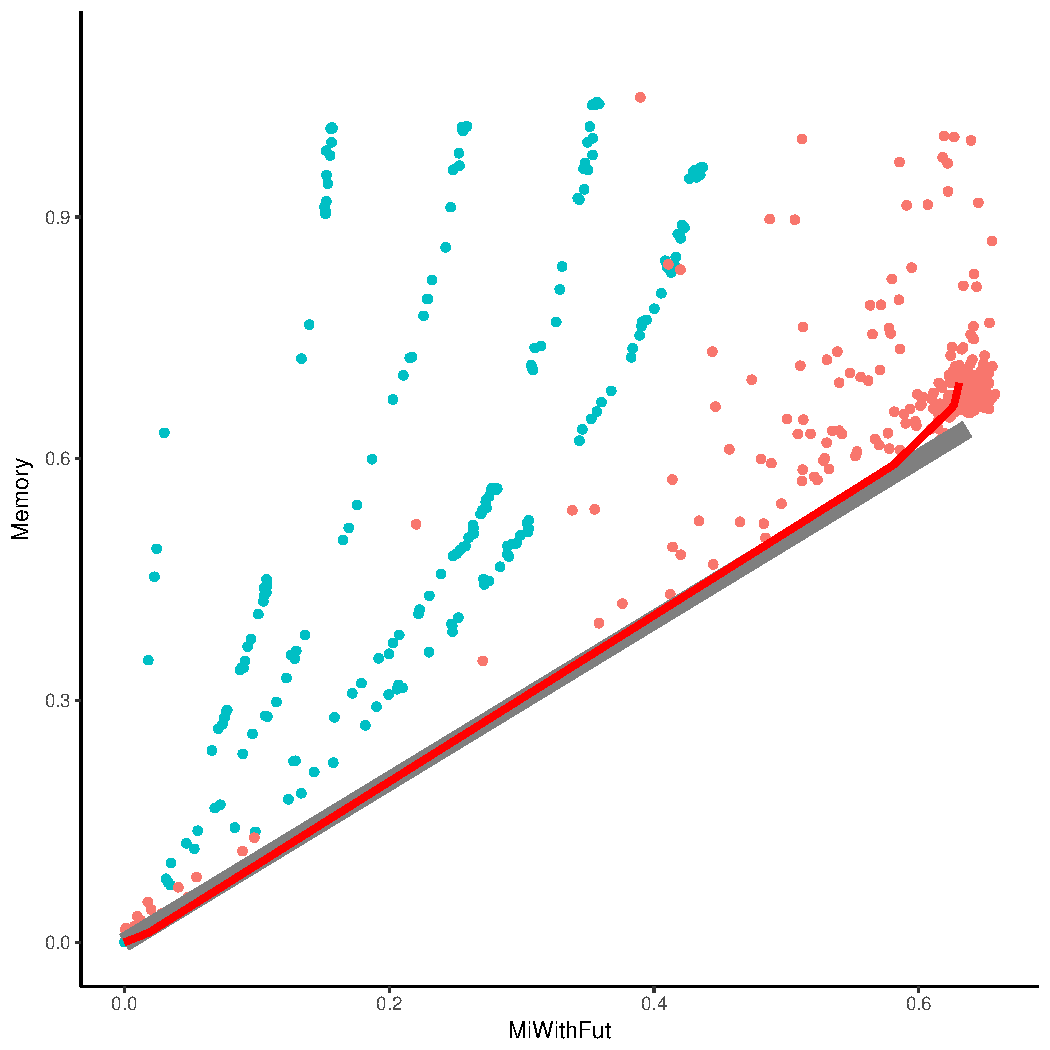
\includegraphics[width=0.45\textwidth]{code/figures/even-info.pdf}
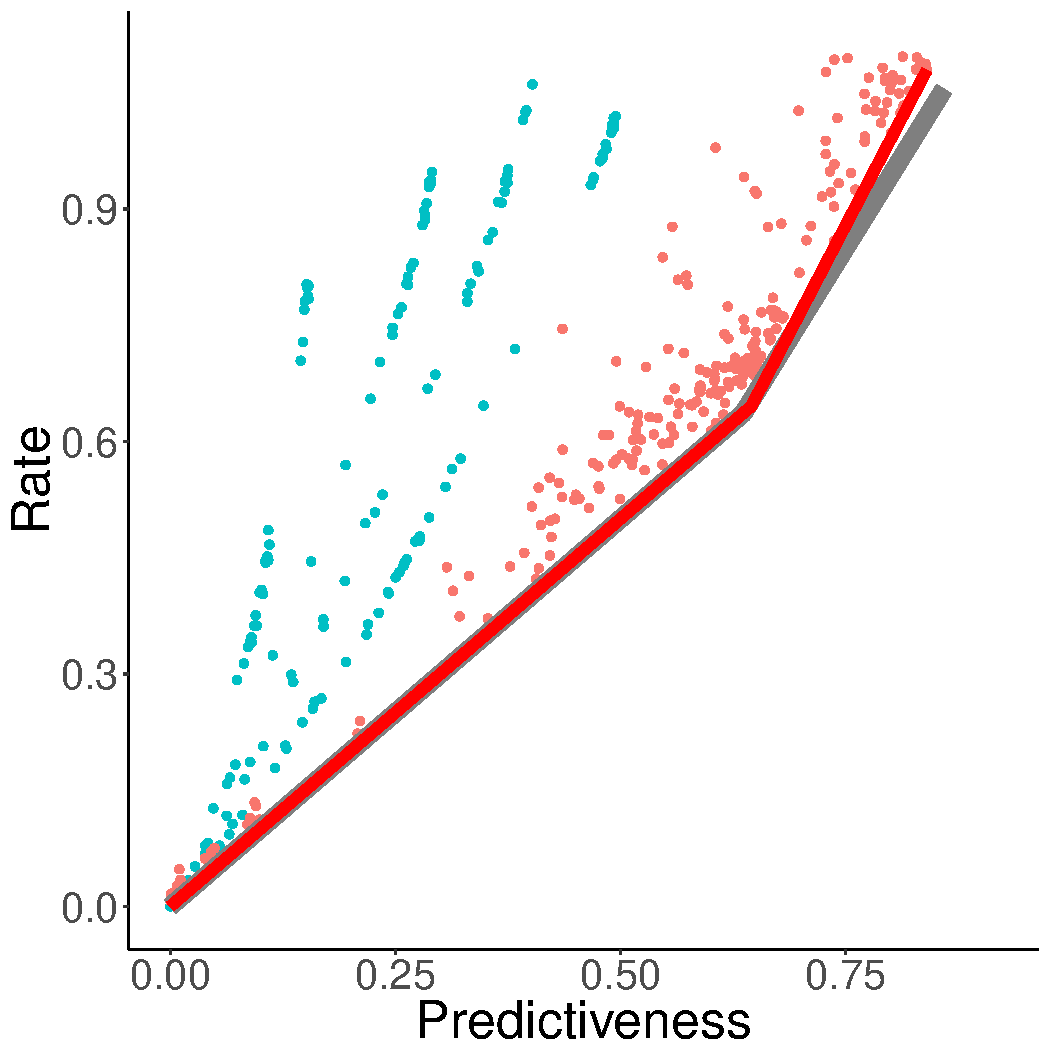
\includegraphics[width=0.45\textwidth]{code/figures/rip-info.pdf}

%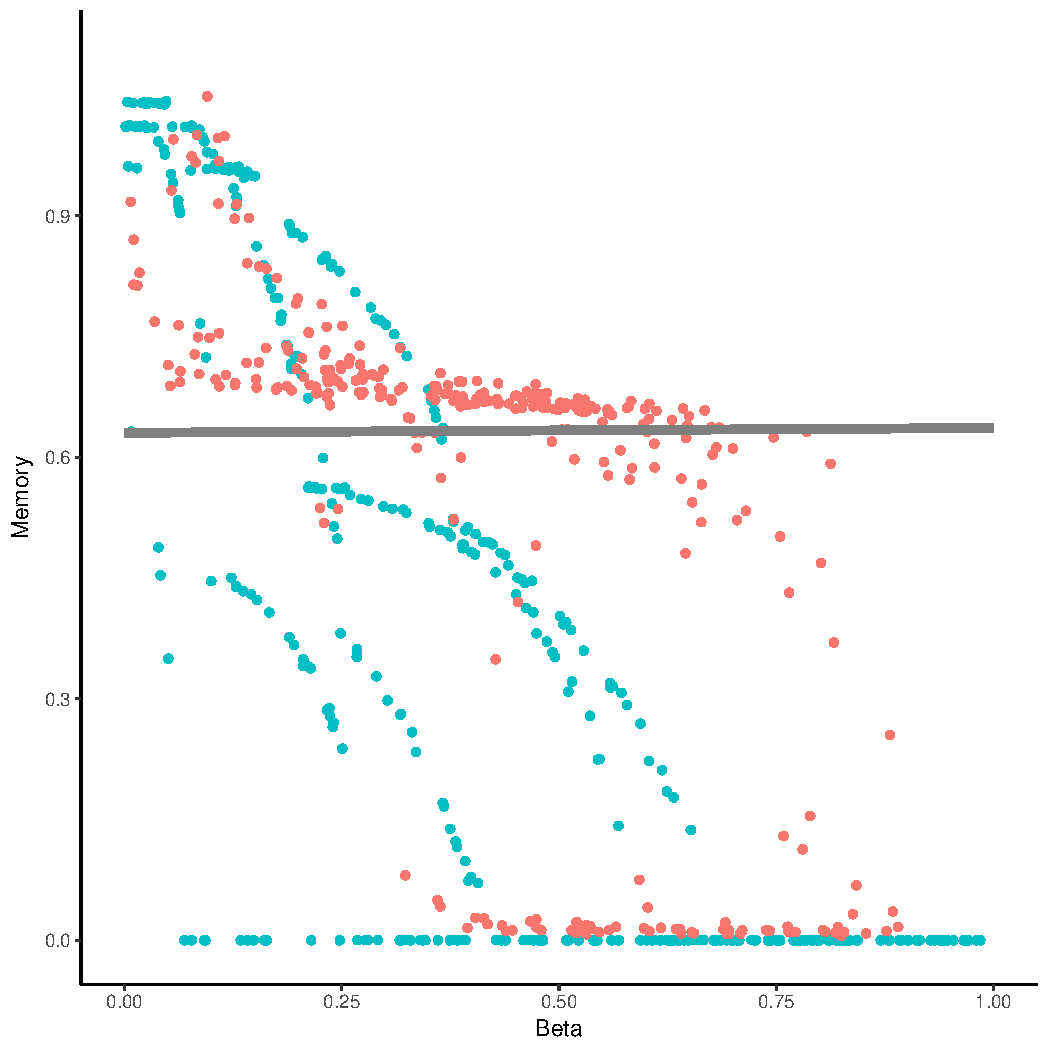
\includegraphics[width=0.45\textwidth]{code/figures/even-beta-mem.pdf}
	\caption{Rate-Distortion for the Even Process and the Random Insertion Process. Gray lines: Analytical curves. Red dots: Multiple runs of NPRD. Red line: Tradeoff curve computed from NPRD runs. Blue: OCE for $M\leq 5$. }\label{fig:even}
\end{figure*}

\paragraph{Recovering Causal States}
Does NPRD lead to inpretable codes $Z$?
To answer this, we further investigated the NPRD approximation to the Random Insertion Process (RIP), obtained in the previous paragraph.
The $\epsilon$-machine was computed by  \cite{marzen-predictive-2016} and is given in Figure~\ref{fig:rip-machine} (right).
The process has three caual states:
A represents those pasts where the future starts with $1^{2k}0$ ($k = 0, 1, 2, \dots$) -- these are the pasts ending in either $001$ or $10111^m$ ($m= 0, 1, 2, \dots$). % but cannot go in with 10
B represents those pasts ending in 10 -- the future has to start with 01 or 11.
C represents those pasts ending in either 00 or 01 -- the future has to start with $1^{2k+1}0$ ($k = 0, 1, 2, \dots$).
%These states represent the 
%As itThis $\epsilon$-machine is the smallest unifilar

The analytical solution to the predictive rate-distortion problem was computed by \cite{marzen-predictive-2016}.
At $\beta > 0.5$, the optimal solution collapses $A$ and $B$ into a single codeword, while all three states are mapped to separate codewords for $\beta \leq 0.5$.


Does NPRD recover this picture?
We applied PCA to samples from $Z$ computed at two different values of $\beta$, $\beta = 0.25$ and $\beta = 0.6$, corresponding to the two points marked in the rate-distortion figure.
The first two principal components are shown in Figure~\ref{fig:latent}.
Samples are colored by the causal states corresponding to the pasts of the trajectories that were encoded into the respective points by NPRD.
On the left, obtained at $\beta=0.6$, the states A and B are collapsed, as expected.
On the right, obtained at $\beta=0.25$, the three causal states are reflected as distinct modes of $Z$.
Note that, at finite $M$, a fraction of pasts is ambiguous between the green and blue causal states; these are colored in black and NPRD maps them into a region between the modes corresponding to these states.

In Figure~\ref{fig:rip-machine}, we record, for each of the three modes to which cluster the distribution of the code $Z$ shifts when a symbol is appended.
We restrict to those strings that have nonzero probability for RIP (no code will ever be needed for other strings).
For comparison, we show the $\epsilon$-machine computed by \cite{marzen-predictive-2016}.
Comparing the two diagrams shows that NPRD effectively recovers the $\epsilon$-machine:
The three causal states are represented by the three different modes of $Z$, and the effect of appending a symbol also mirrors the state transitions of the $\epsilon$-machine.

\begin{figure*}
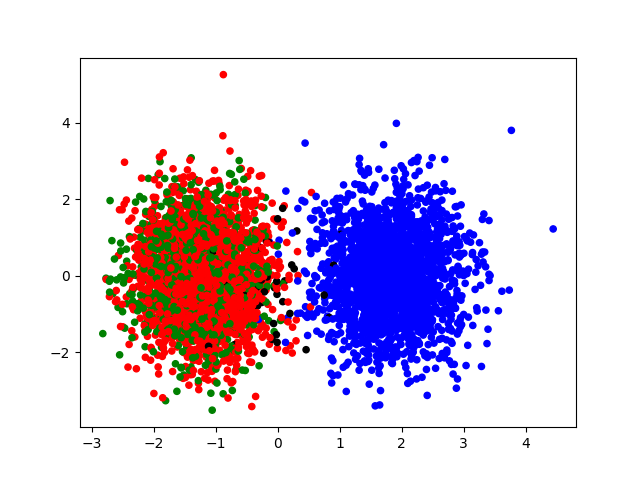
\includegraphics[width=0.45\textwidth]{code/figures/foo_pca_2.png}
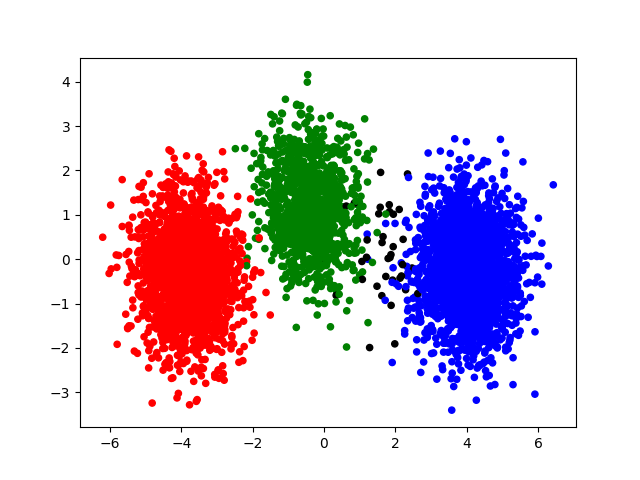
\includegraphics[width=0.45\textwidth]{code/figures/foo_pca_3.png}
	\caption{Applying PCA to 5000 sampled codes $Z$ for the Random Insertion Process, at $\beta = 0.25$ and $\beta = 0.6$. Samples are colored according to the states in the $\epsilon$ machine. Black samples belong to sequences that, at $M=15$, cannot be uniquely attributed to any of the states (ambiguous between A and C).}\label{fig:latent}
\end{figure*}
% colors = [{"A" : "red", "B" : "green", "C" : "blue", "U" : "black"}[x] for x in states]

\begin{figure*}
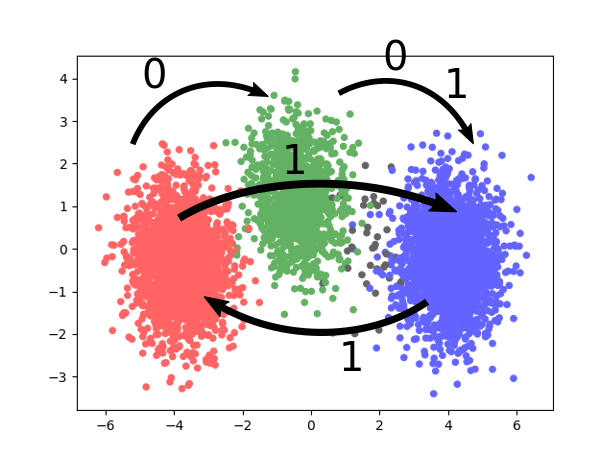
\includegraphics[width=0.45\textwidth]{code/figures/foo_pca_3_machine.png}
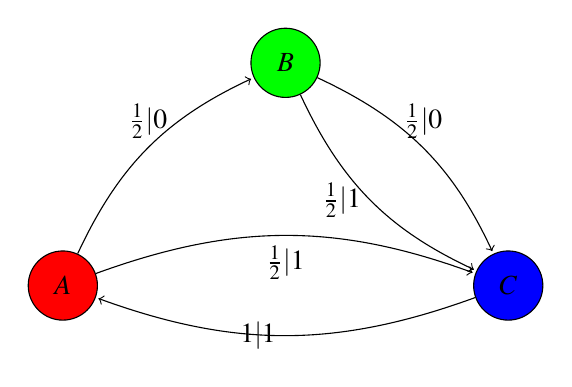
\begin{tikzpicture}[shorten >=1pt,node distance=4cm,on grid,auto] 
   \node[state, fill=green] (B)   {$B$}; 
   \node[state, fill=red] (A) [below left=of B] {$A$}; 
   \node[state, fill=blue] (C) [below right=of B] {$C$}; 
    \path[->] 
	(A) edge [bend left=20] node [above] {$\frac{1}{2} | 0$} (B)
	(A) edge [bend left=20] node [below] {$\frac{1}{2} | 1$} (C)
	(B) edge [bend left=20] node [above] {$\frac{1}{2} | 0$} (C)
	(B) edge [bend right=20] node [left] {$\frac{1}{2} | 1$} (C)
	(C) edge [bend left=20] node [left] {$1 | 1$} (A)
	;
%
%%          edge  node [swap] {1} (B)
%    (C) edge  node  {1} (A)
%          edge [loop above] node {0} ()
%	(A) edge  node [swap] {0} (C) 
%          edge [loop below] node {1} ();
\end{tikzpicture}


	\caption{Left: Recovering the $\epsilon$ machine from NPRD: By recording how the code $Z$ changes when a symbol is appended to a past $x_{-15\dots-1}$, we recover the epsilon machine described by \cite{marzen-predictive-2016}. Right: The epsilon machine.}\label{fig:rip-machine}
\end{figure*}






%- p. 14 in https://arxiv.org/pdf/1412.2859.pdf

%\paragraph{RRXOR}
%
%
%The process of pairs ABC where $C = A xor B$.
%Stationary.
%We additionally interspersed blocks of neutral letters with geometric length.
%
%36 causal states
%
%%As   an   example,   consider   the   random-random   XOR
%%
%%RRXOR
%%
%%process  that  consists  of  two  successive  random
%%symbols  chosen  to  be  0  or  1  with  equal  probability  and  a
%%third symbol that is the logical exclusive-OR
%%
%%XOR
%%
%%of the
%%two previous. The RRXOR process can be represented by a
%%hidden  Markov  chain  with  five  recurrent  causal  states,  but
%%having a much larger total number of causal states. There are
%%36 causal states, most
%%
%%31
%%
%%of which describe a complicated
%%transient  structure.
%%27
%%As  such,  it  is  a  structurally  complex
%%process  that  an  analyst  may  wish  to  approximate  with  a
%%smaller set of states.
%
%%          for _ in range(10000 if partition == "dev" else 100000):
%%              a = (random.random() > 0.5)
%%              b = (random.random() > 0.5)
%%
%%              while random.random() > 0.9: # randomness makes it stationary
%%                  data[-1].append(encode("2"))
%%              data[-1].append(encode("1" if a else "0"))
%%              while random.random() > 0.9:
%%                  data[-1].append(encode("2"))
%%              data[-1].append(encode("1" if b else "0"))
%%              while random.random() > 0.9:
%%                  data[-1].append(encode("2"))
%%              data[-1].append(encode("1" if a != b else "0"))
%%
%
%
%
%\paragraph{Process with Low Excess Entropy and High Memory}
%
%the one we talked about recently (TODO)
%
%

\paragraph{A Process with Many Causal States}
We have seen that NPRD recovers the correct tradeoff, and the structure of the causal states, in processes with a small number of causal states.
How does it behave when the number of causal states is very large?
In particular, is it capable of extrapolating to causal states that were never seen during training?

We consider the following process, which we'll call \textsc{Copy3}: $X_{-15}, ..., X_{-1}$ are independent uniform draws from $\{1,2,3\}$, and $X_1 = X_{-1}, ..., X_{15} = X_{-15}$.
This process deviates a bit from our usual setup since we defined it only for $t \in \{-15, ..., 15\}$, but it is well-suited to investigating this question:
The number of causal states is $3^{15} \approx 14$ million.
With exactly the same setup as for the \textsc{Even} and \textsc{RIP} processes, NPRD achieved essentially zero distortion on unseen data, even though the number of training samples (3 Million) was far lower than the number of distinct causal states.
However, we found that, at this setup, NPRD overestimated the rate.
Increasing the number of training samples from 3M to 6M, NPRD recovered codebooks that achieved both almost zero distortion and almost optimal rate, on fresh samples (Figure~\ref{fig:repeat}).
Even then, the number of distinct causal states is more than twice the number of training samples.
These results demonstrate that, by using function approximation, NPRD is capable of extrapolating to unseen causal states, encoding and decoding appropriate codes on the fly.


Note that one could easily design an optimal decoder and encoder for \textsc{Copy3} by hand -- the point of this experiment is to demonstrate that NPRD is capable of inducing such a codebook purely from data, in a general-purpose, off-the-shelf manner.
This contrasts with OCE:
Without optimizations specific to the task at hand, a direct application of OCE would require brute-force storing of all 14 million distinct pasts and futures.



\begin{figure*}
%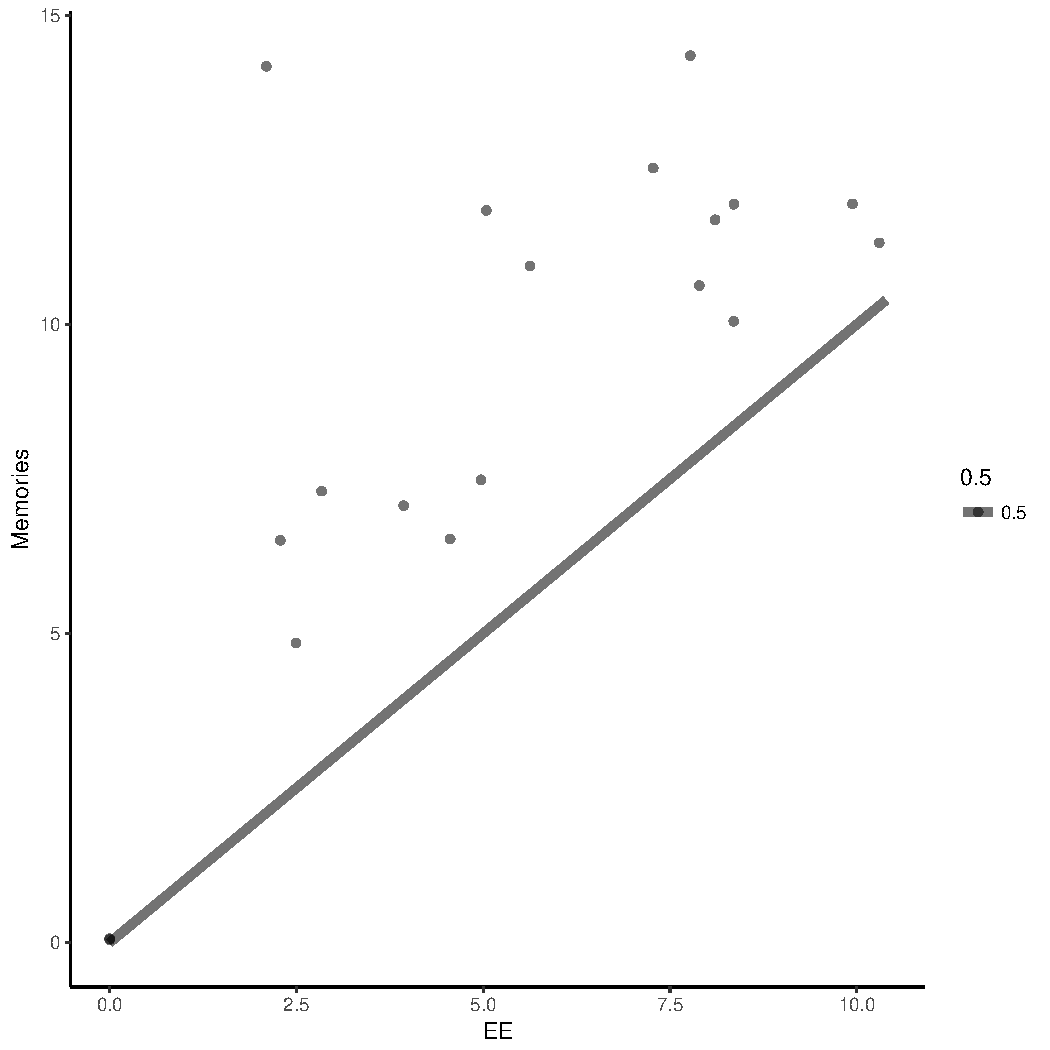
\includegraphics[width=0.45\textwidth]{code/figures/repeat2-ee-mem.pdf}
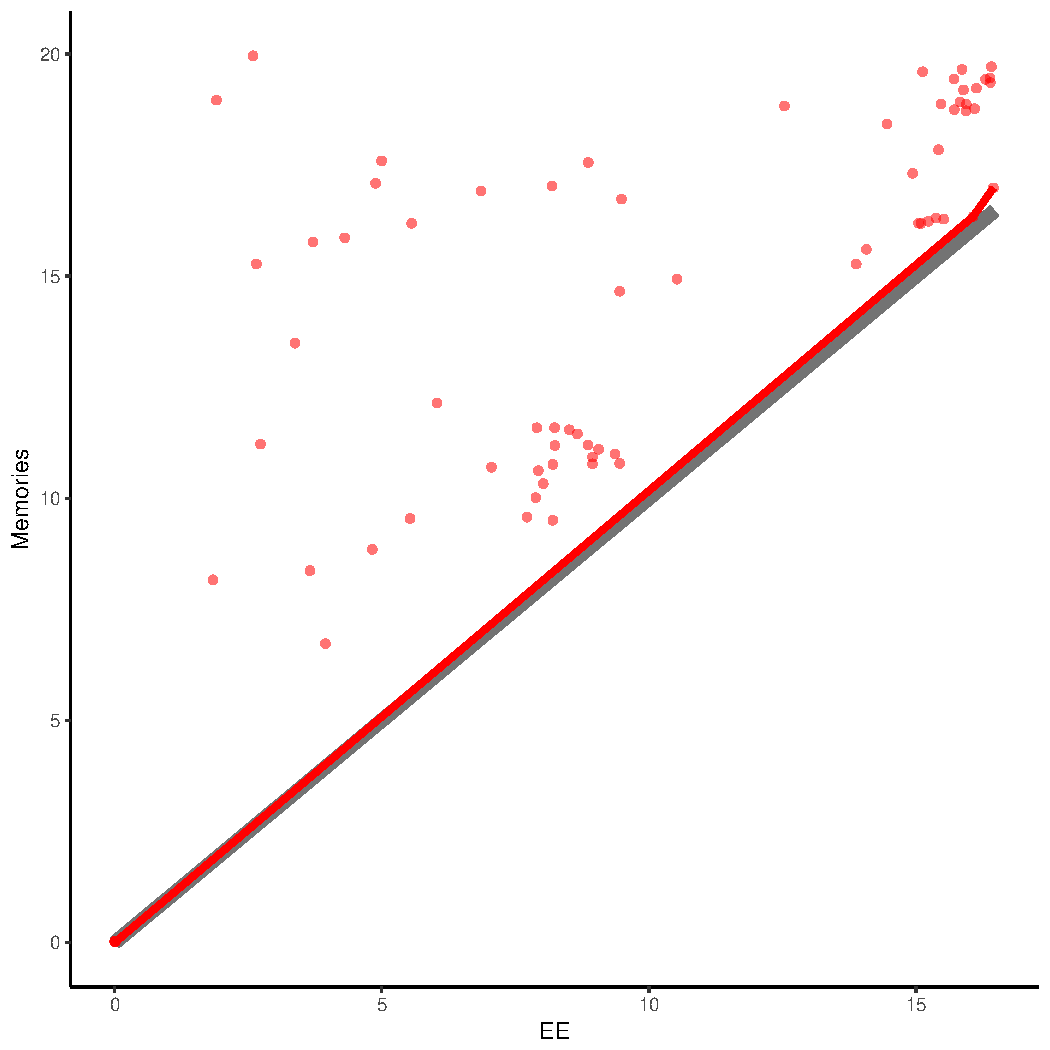
\includegraphics[width=0.45\textwidth]{code/figures/repeat3-ee-mem-frontier.pdf}
	\caption{Rate-Distortion for the \textsc{Copy3} process. We show NPRD samples, and the resulting upper bound in red. The gray line represents the anaytical curve.}\label{fig:repeat}
\end{figure*}
%  \rljf{Red not green? Also y axis should be Memory, not Memories. Also let's label as Memory (nats) throughout (or bits), and Excess Entropy on the x axis throughout.}



\section{Natural Language}

We consider the problem of estimating rate-distortion for Natural Language.

TODO Motivation

UID

%Fenk, A.; Fenk, G. Konstanz im Kurzzeitgedächtnis-Konstanz im sprachlichen Informationsfluß. Z. Exp. Angew. Pshychol. 1980, 27, 400–414.
%Fenk-Oczlon, G. Familiarity, information flow, and linguistic form. In Frequency and the Emergence of Linguistic Structure; Bybee, J.L., Hopper, P.J., Eds.; John Benjamins: Amsterdam, The Netherlands, 2001; pp. 431–448.
%Ferrer-i Cancho, R.; D ̨ebowski, Ł.; del Prado Martín, F.M. Constant conditional entropy and related hypotheses. J. Stat. Mech. Theory Exp. 2013, L07001, doi:10.1088/1742-5468/2013/07/L07001.

People have studied information density as a model of cost in human language processing.

But also memory cost is relevant

\cite{bentz2017entropy}

\cite{koplenig2017statistical}

\cite{dkebowski2018natural}

\cite{takahira2016entropy}

\rljf{Some motivation for why this is cool and interesting, maybe in parallel with the Bentz et al entropy paper, and other information theoretic linguistic complexity papers like Koplenig et al, and Dembowski's work}

\subsection{Part-of-speech-level language modeling}

We first consider the problem of predicting English on the level of Part-of-Speech (POS) tags, using the Universal POS tagset \citep{petrov-universal-2012}. 
This is a simplified setting where the vocabulary is small (20), and one can hope that OCE will produce reasonable results.
We use the English portions of the Universal Dependencies Project~\citep{nivre-universal-2017} tagged with Universal POS Tags \citep{petrov-universal-2012}, consisting of approximately 586K words.
We used the training portions to estimate NPRD and OCE, and the validation portions to estimate rate-distortion.
We used NPRD to generate 350 codebooks for values of $\beta$ sampled from [0,0.4].
We were only able to run OCE for $M \leq 3$, as the number of sequences exceeds $10^4$ already at $M=4$.


The information curve is shown in Figure~\ref{fig:eng-pos} (left).
In the setting of low rate and high distortion, NPRD and OCE ($M=3$) show essentially identical results.
This holds true until $I[Z, \overrightarrow{X}] \approx 0.7$, at which point the bounds provided by OCE deteriorate, showing the effects of overfitting.
NPRD continues to provide estimates at greater rates.

Figure~\ref{fig:eng-pos} (right) shows rate as a function of $\beta$.
In Figure~\ref{fig:eng-logbeta}, we show rate and the mutual information with the future, as a function of $\log \frac{1}{\beta}$.
Recall that $\beta$ is the tradeoff-parameter from the objective function~\ref{eq:ib}.
As $\beta \rightarrow 0$, NPRD (red, $M=15$) continues to discover structure, while OCE (blue, plotted for $M=1,2,3$) exhausts its capacity.

Note that NPRD reports rates of 15 nats and more when modeling with very low distortion.
A discrete codebook would need over 3 million distinct codewords for a code of such a rate, exceeding the size of the training corpus (about 500K words), replicating what we found for the \textsc{Copy3} process:
Neural encoders and decoders can use the continuous geometric structure of the code space to encode generalizations across different dimensions, supporting a very large effective number of distinct possible codes.
Unlike discrete codebooks, the geometric structure makes it possible for neural encoders to construct appropriate codes `on the fly' on new input.



\begin{figure*}
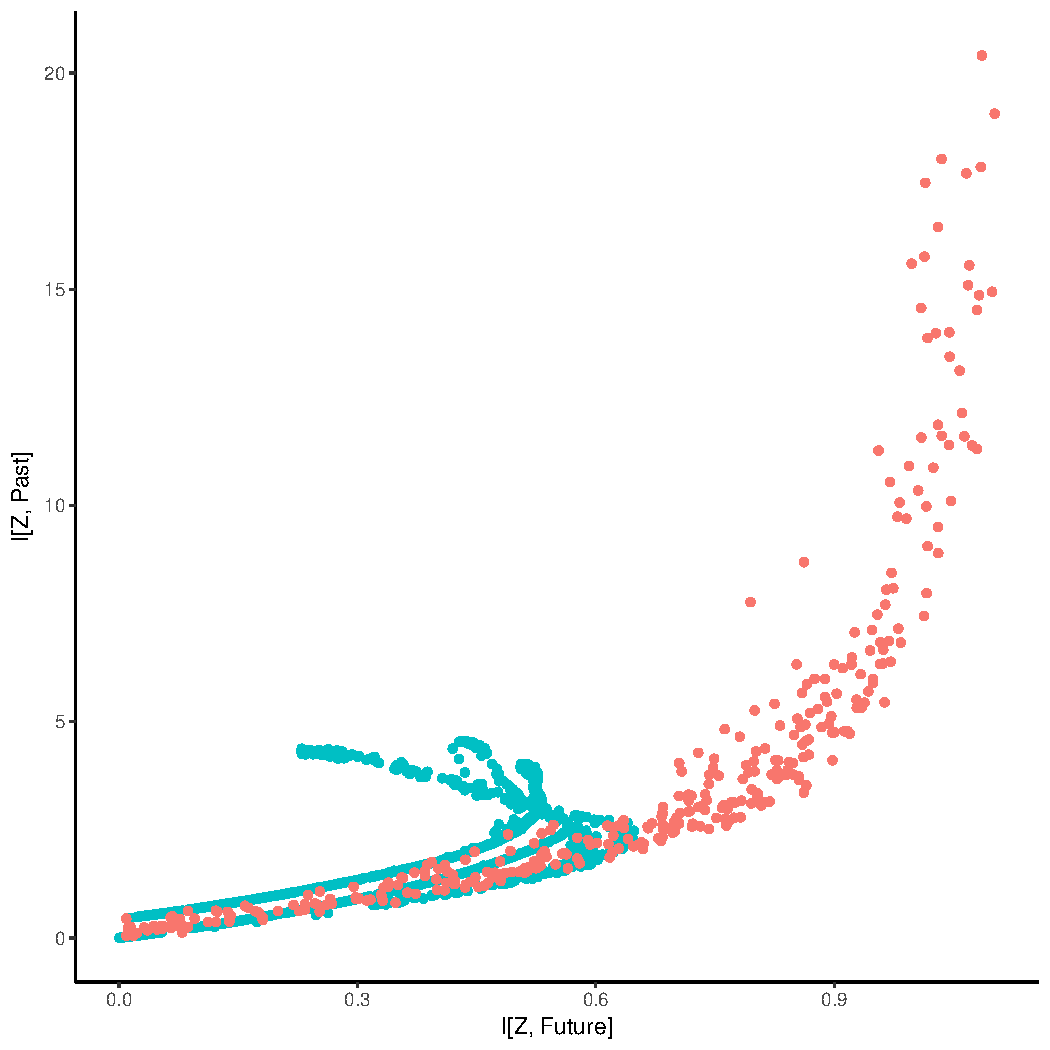
\includegraphics[width=0.3\textwidth]{code/figures/english-info.pdf}
%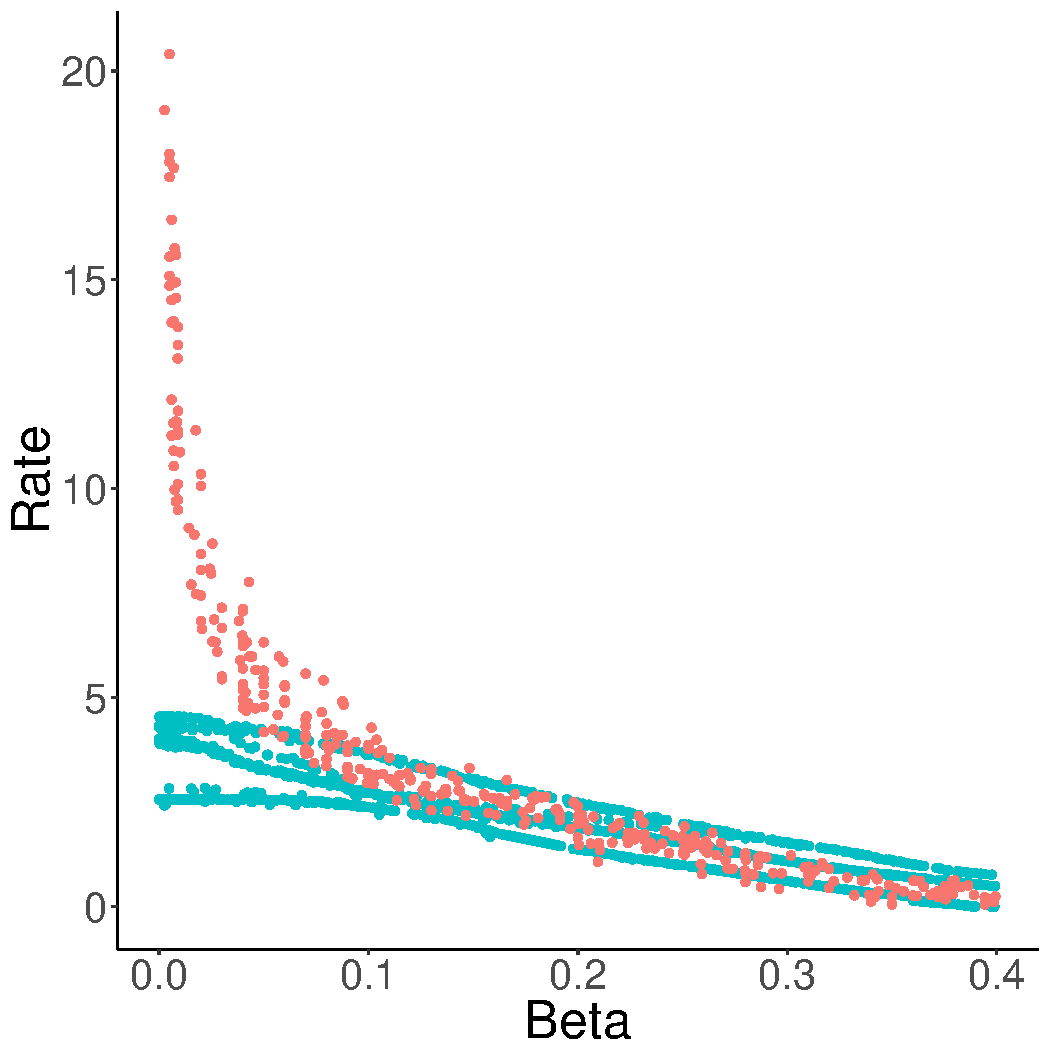
\includegraphics[width=0.45\textwidth]{code/figures/english-beta-mem.pdf}
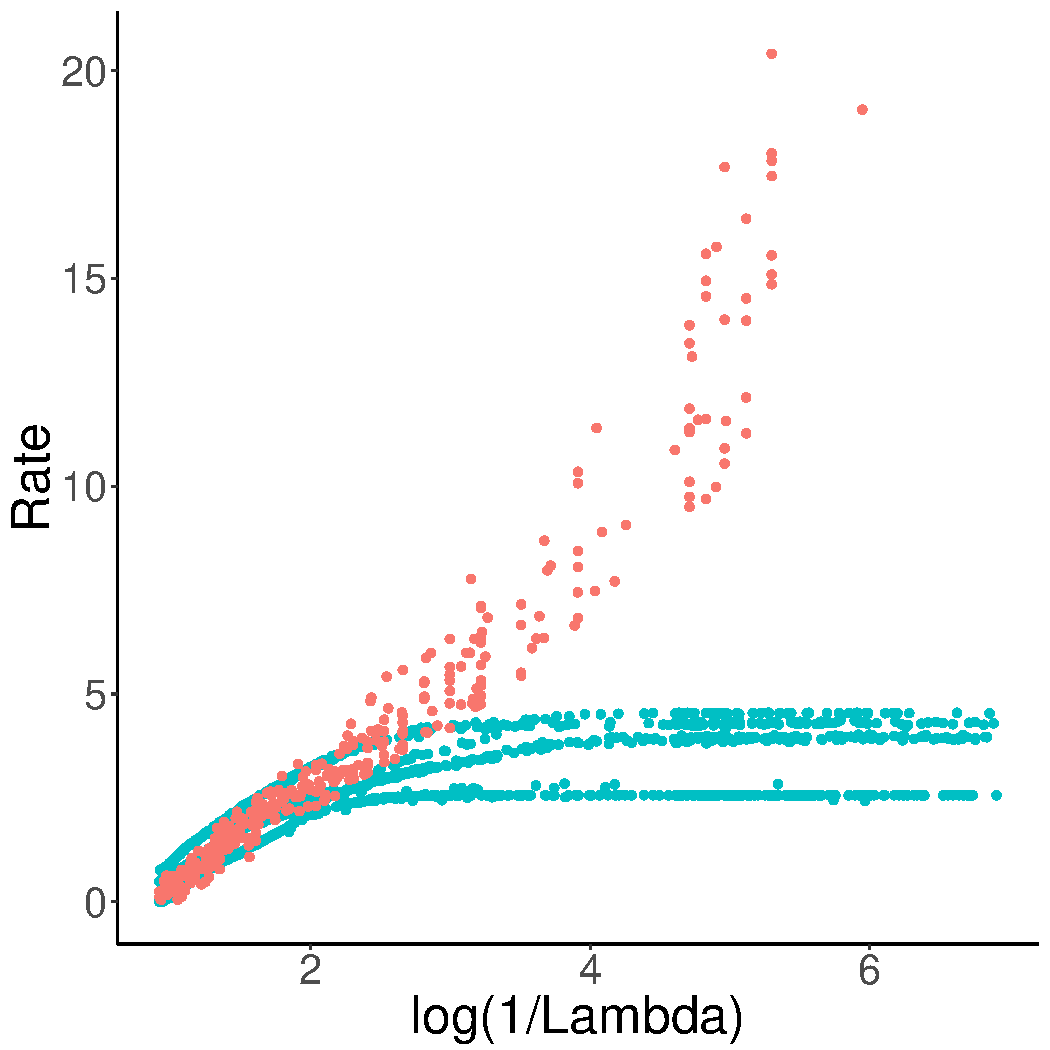
\includegraphics[width=0.3\textwidth]{code/figures/english-nlogbeta-mem.pdf}
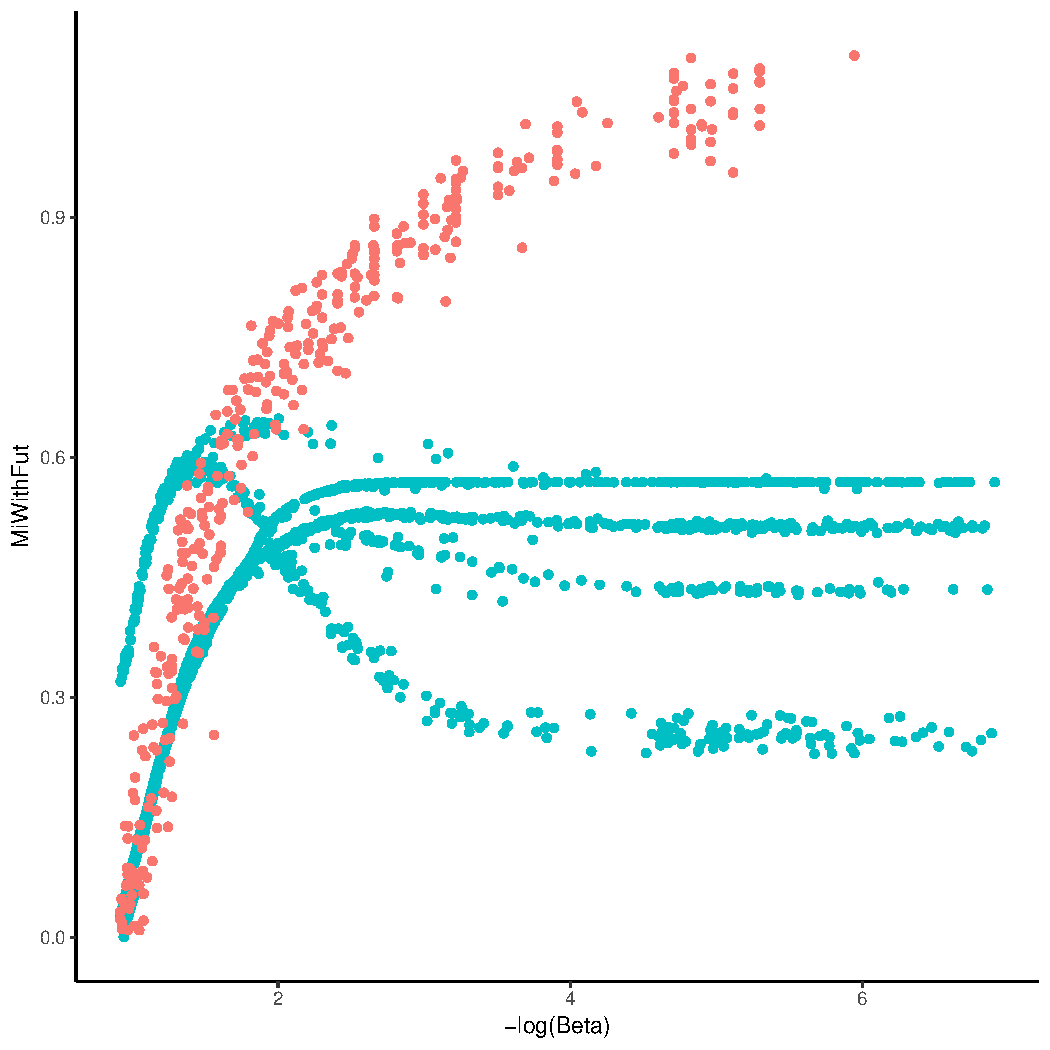
\includegraphics[width=0.3\textwidth]{code/figures/english-nlogbeta-ee.pdf}
	\caption{Left: Rate-Predictiveness for English POS modeling. Center and right: Rate (center) and Predictiveness (right) on English POS Modeling, as a function of $-\log \beta$. As $\beta \rightarrow 0$, NPRD (red, $M=15$) continues to discover structure, while OCE (blue, plotted for $M=1,2,3$) exhausts its capacity.}\label{fig:eng-pos}
\end{figure*}



\subsection{Discussion}
Let us now interpret the curves in Figure~\ref{fig:eng-pos}. \rljf{What is predictiveness? Excess entropy?}
The rate-predictiveness curve (left) shows that, at low rates, predictiveness is approximately proportional to the rate.
At greater degrees of predictiveness, rate grows faster and faster, whereas predictiveness seems to asymptote to $\approx 1.1$ nats.
%(In the case of our experiment, since $T = 15$, rate would be bounded by the aggregate block-entropy of 15 words, about 28 nats.)
The asymptote of predictiveness can be identified with the excess entropy, whereas the rate should asymptote to the statistical complexity.
Judging by the curve, natural language---at the level we are measuring in this experiment---has a statistical complexity much higher than its excess entropy:
At the highest rate measured by NPRD in our experiment, rate is about 20 nats, whereas predictiveness is about 1.1 nats.
If these values are correct, then---due to the convexity of the rate-predictivity curve---statistical complexity exceeds the excess entropy by a factor of at least $\frac{20}{1.1}$. \rljf{Wow, is this true for any other natural processes?}
Note that this picture agrees qualitatively with the OCE results, which suggest a lower-bound on the ratio of at least $\frac{2.5}{0.6} > 5$.

Now turning to the other plots in Figure~\ref{fig:eng-pos}, we observe that rate increases at least linearly with $\log\lambda$, whereas predictiveness again asymptotes.
This is in qualitative agreement with the picture gained from the rate-predictiveness curve.


Let us consider this more quantitatively.
Based on Figure~\ref{fig:eng-pos} (center), we make the guess that the map from $\log\lambda$ to the rate $R$ is superlinear:
\rljf{Was there a change of variables between $\beta$ and $\lambda$ here?}
\begin{equation}
	R = \alpha (\log\lambda)^\beta
\end{equation}
	with $\alpha>0, \beta>1$.
We fitted $R \approx (\log\lambda)^{1.7}$.

Equivalently
\begin{equation}
\lambda = \exp\left(\frac{1}{\alpha^{1/\beta}} M^{1/\beta}\right)
\end{equation}
From this, we can derive expressions for rate $R$ and predictiveness $P$ as follows.
For the solution of Predictive Rate Distortion, we have
\begin{equation}
	\frac{\partial P}{\partial \theta} - \lambda \frac{\partial R}{\partial \theta} = 0,
\end{equation}
where $\theta$ is the codebook defining the code $Z$, and thus
\begin{equation}
\lambda =	\frac{\partial P}{\partial R}.
\end{equation}

Thus
\begin{equation}\label{eq:derivatives}
	\partial P/\partial R = \exp\left(-\frac{1}{\alpha^{1/\beta}} R^{1/\beta}\right). %&\ \ \ \partial R/\partial P = \exp\left(\frac{1}{\alpha^{1/\beta}} R^{1/\beta}\right)
\end{equation}
Qualitatively, this says that $P$ asymptotes to a finite value, whereas $R$ is unbounded. \rljf{Exactly the opposite of Dembowski's finding}



\begin{figure*}
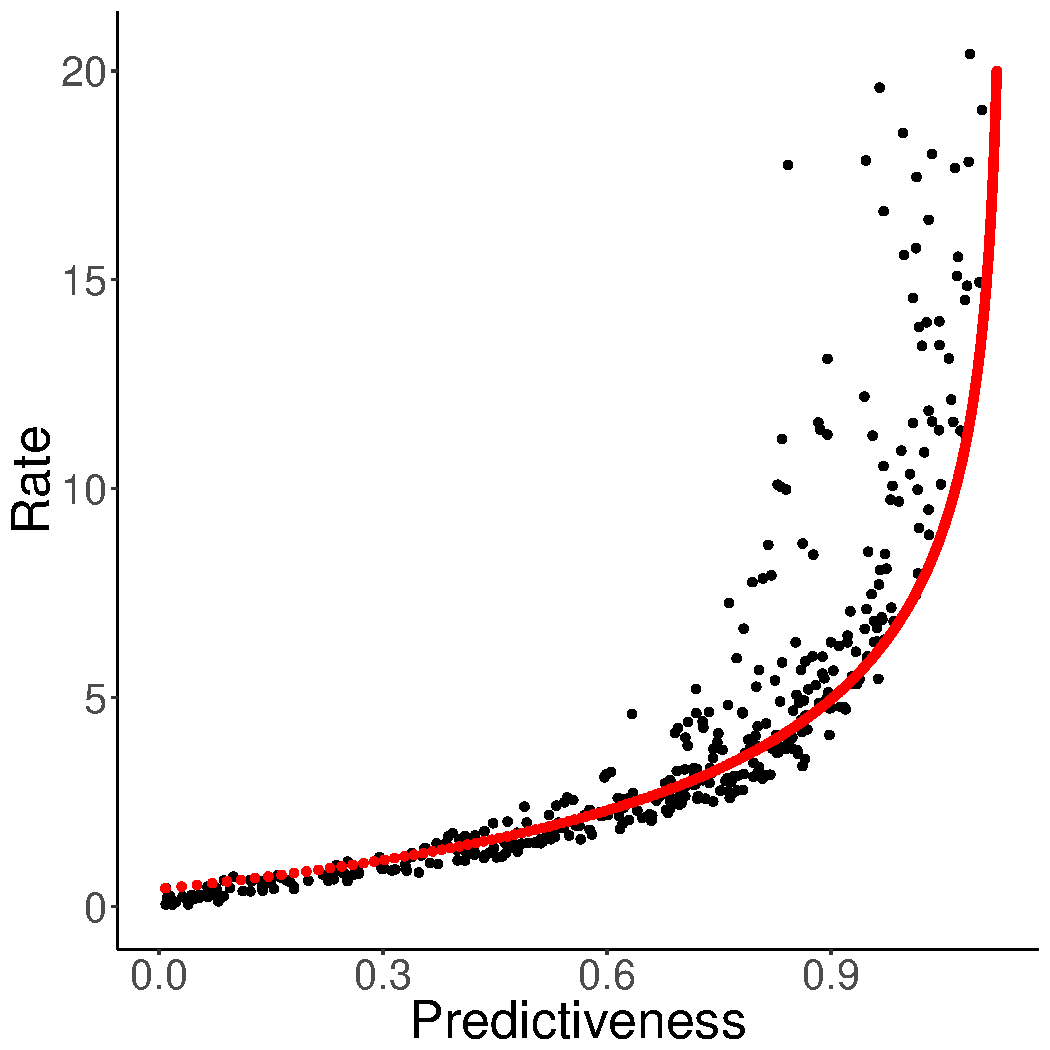
\includegraphics[width=0.3\textwidth]{code/figures/english-info-fitted.pdf}
%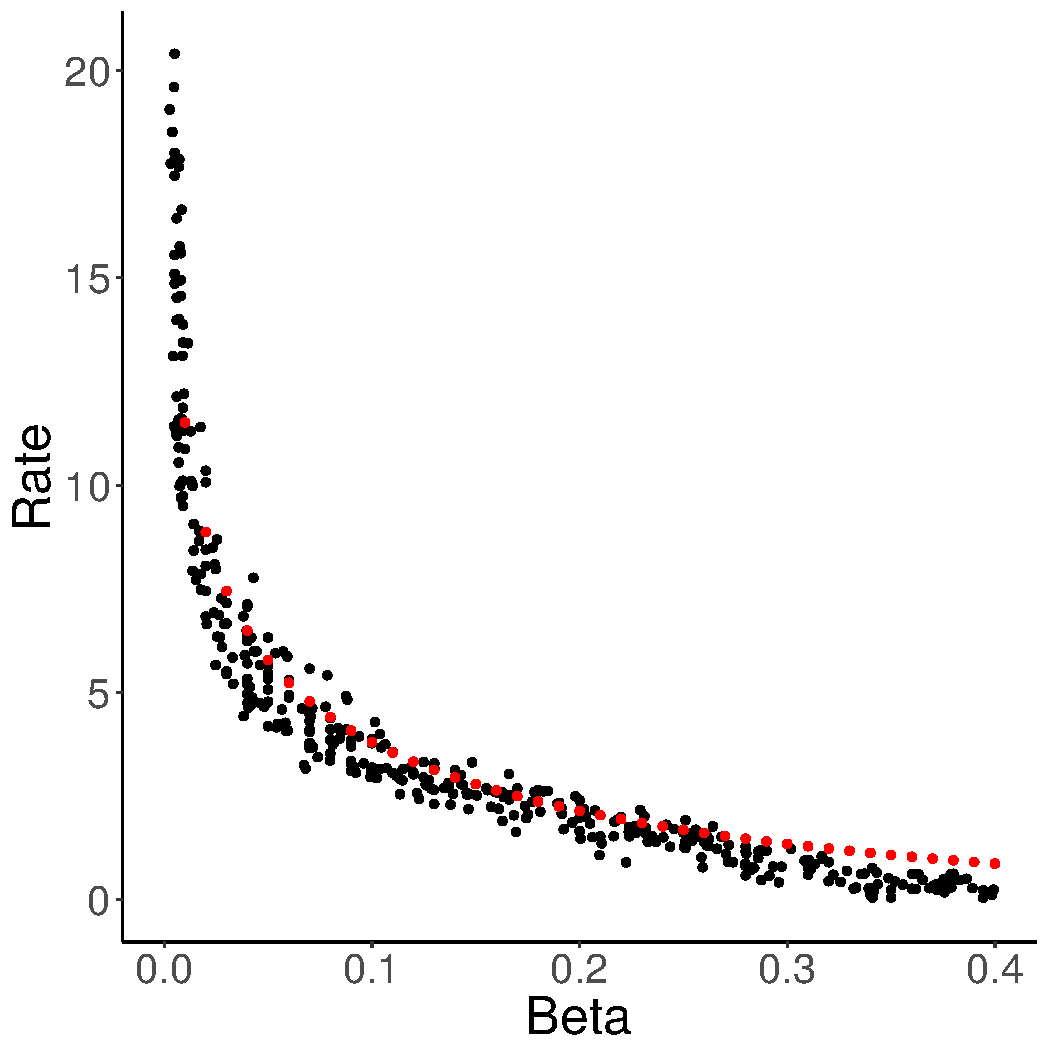
\includegraphics[width=0.45\textwidth]{code/figures/english-beta-mem-fitted.pdf}
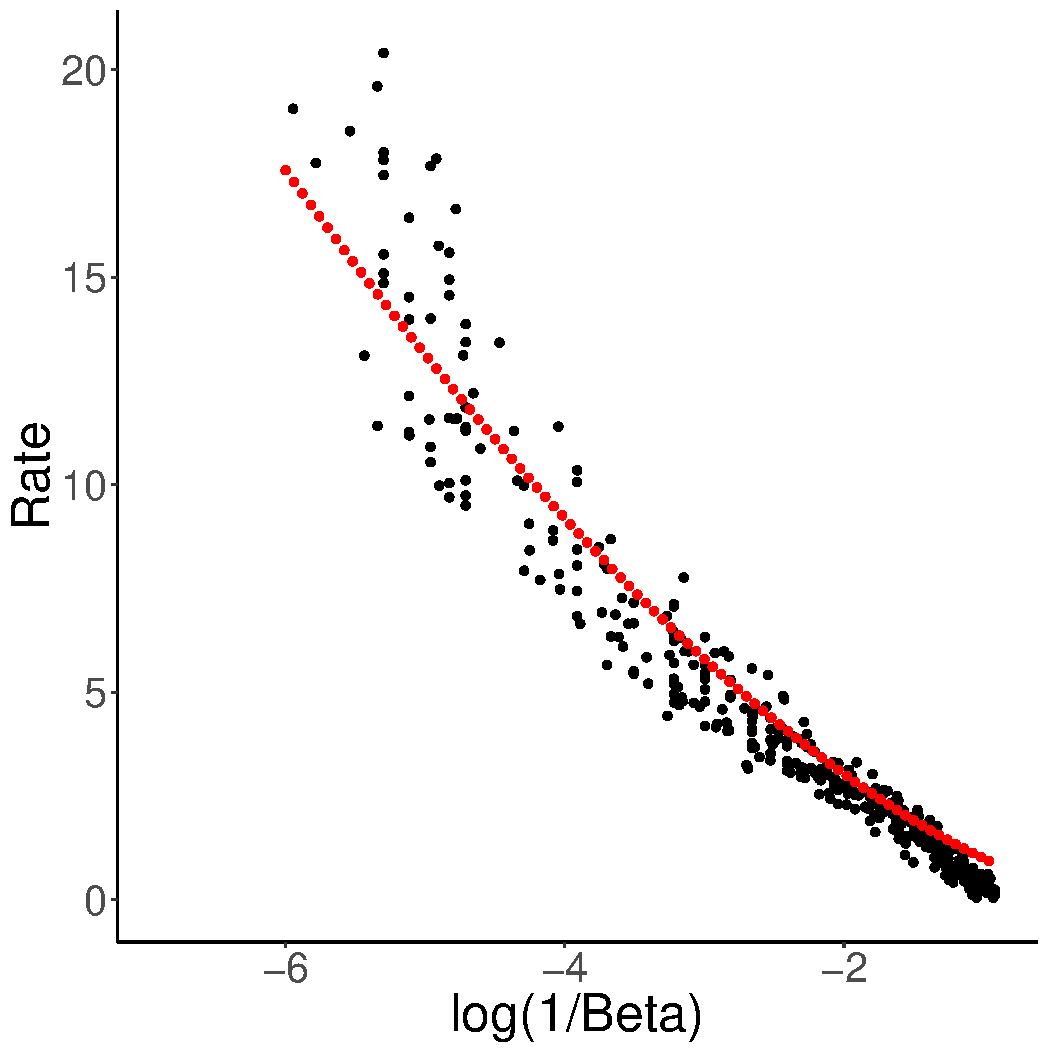
\includegraphics[width=0.3\textwidth]{code/figures/english-logbeta-mem-fitted.pdf}
	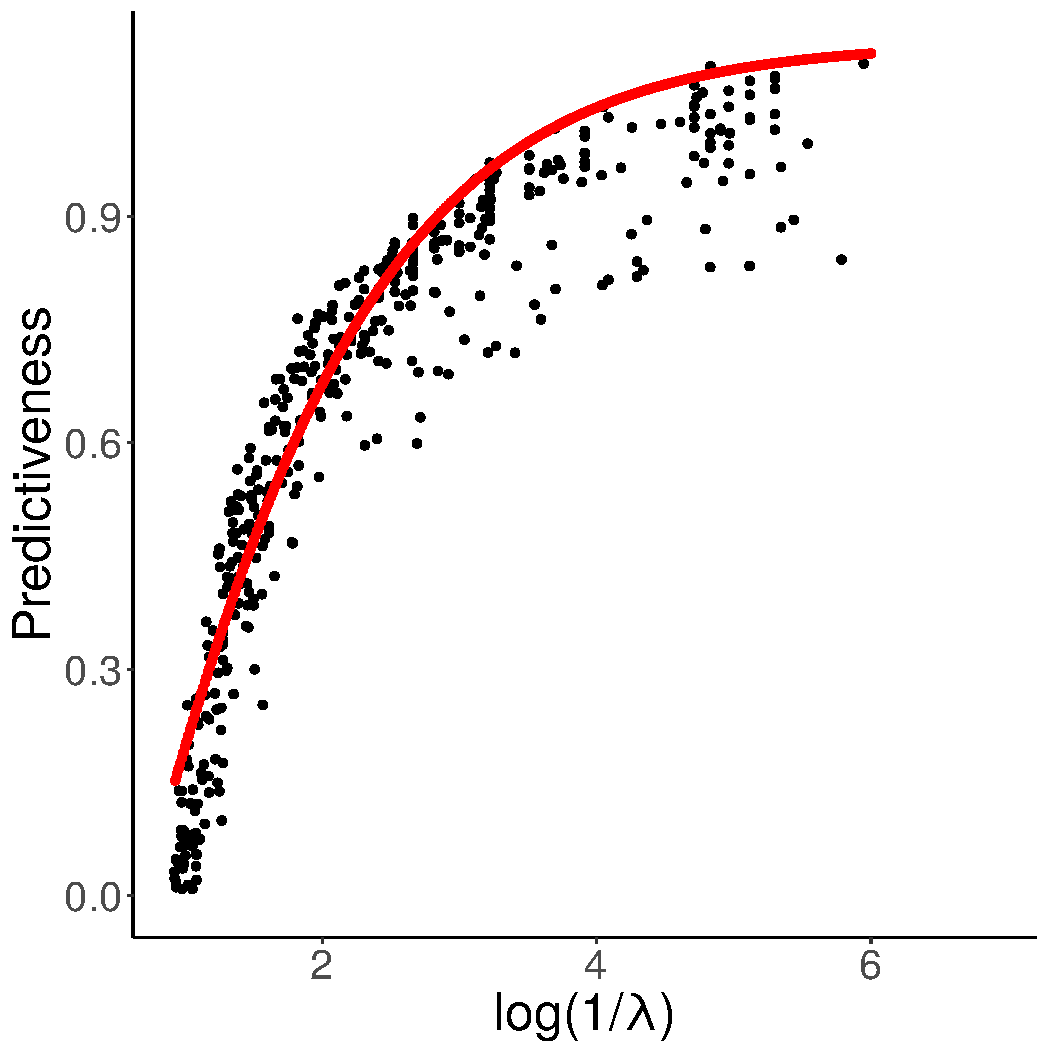
\includegraphics[width=0.3\textwidth]{code/figures/english-nlogbeta-ee-fitted.pdf}
	\caption{Fitted values. \rljf{Definitely need a better label, also axis labels are too small to read}}\label{fig:eng-pos-fitted}
\end{figure*}

This yields
\begin{equation}
	P = C - \alpha\beta \cdot \Gamma\left(\beta, (R/\alpha)^{1/\beta}\right)
\end{equation}
where $\Gamma$ is the incomplete Gamma function.
Since $\lim_{R \rightarrow \infty} P = C$, we can identify the constant $C$ with the excess entropy $I[\overleftarrow{X}, \overrightarrow{X}]$ of the process.

As $M \rightarrow \infty$, this behaves as
\begin{equation}
	P \approx E_0 - \alpha\beta \cdot (R/\alpha)^{\frac{\beta-1}{\beta}} e^{-(R/\alpha)^{1/\beta}}
\end{equation}
which asymptotes to $E_0$.
We found that $\beta = 1.7$, $E_0 = 1.13$ yielded a good fit.
This can be extended without further parameters to the third curve in Figure~\ref{fig:eng-pos}.
Resulting fits are shown in Figure~\ref{fig:eng-pos-fitted}.
%$E = E_0 - \Gamma(1.6, (\log\beta))$

Note that there are many possible ways of fitting these curves; we have described a simple one that requires two free parameters $\alpha >0$, $\beta > 1$, in addition to a guess for the excess entropy $E_0$.
In any case, the results show that natural language shows an approximately linear growth of predictiveness with rate at small rates, and exploding rates at diminishing returns in predictiveness later.
Why might language show such behavior?
We will describe a proposal:
Let us assume that the causal states of natural language are the singletons $\overleftarrow{X}$, that is, no two past trajectories induce a fully equivalent distribution over future trajectories.
Then the code $Z^{(T)}$ which stores the block $X_{-T...-1}$ achieves predictiveness \rljf{Write out what the min is doing logically: when $t$ exceeds $T$ we multiply only by $T$ (I'm not sure why). Also maybe subscript $P_T$}
\begin{equation}
	P =	I[X_{-T...-1}, \overrightarrow{X}]
\end{equation}
By writing $I_t := I[X_0, X_t | X_1 ... X_{t-1}]$, and repeatedly applying the chain rule of conditional mutual infomation, we obtain
\begin{equation}
	P = \sum_{t_- = -T}^{-1} \sum_{t_+ = 0}^\infty I[X_{t_+},X_{t_-}|X_{t_-+1}\dots X_{t_+-1}] = \sum_{t_- = -T}^{-1} \sum_{t_+ = 0}^\infty I_{t_+-t_-}  = \sum_{t=1}^\infty \min(t,T) I_t = E_0 - \sum_{t > T} (t-T) I_t
\end{equation}
where $E_0$ is again the excess entropy.
Again, this asymptotes to the excess entropy, but---as long as $I_t > 0$ for arbitarily large $t$---never achieves predictiveness $E_0$ at finite $T$.
The code has rate
\begin{equation}
	R =	H[X_{-T...-1}]
\end{equation}
which is lower bounded by $T$ times the entropy rate: $R \approx T \cdot \operatorname{H}[X_0|\overleftarrow{X}]$, and thus is unbounded (if the entropy rate is nonzero).
TODO \rljf{A few cites on previous work arguing about whether natural language has nonzero entropy rate. A conference paper by Ryosuke Takahira has a lit review}

Approximating $t$ as a continuous variable, we can write
\begin{equation}
	P =	E_0 - \int_{t > T} (t-T) I_t
\end{equation}
\begin{equation}
	\frac{\partial P}{\partial T} =	\int_{t > T} I_t
\end{equation}
\begin{equation}
	\frac{\partial R}{\partial T} \approx \operatorname{H}[X_0|\overleftarrow{X}]
\end{equation}
and thus
\begin{equation}
	\frac{\partial P}{\partial R} \approx	\frac{1}{\operatorname{H}[X_0|\overleftarrow{X}]} \int_{t > T} I_t
\end{equation}
Matching this with~(\ref{eq:derivatives}), we get
\begin{equation}
	\exp\left(-T^{1/\beta} \frac{1}{\alpha^{1/\beta}} (\operatorname{H}[X_0|\overleftarrow{X}])^{1/\beta}\right) \propto \int_{t > T} I_t
\end{equation}
and thus
\begin{equation}
I_t \propto T^{1/\beta-1}	\exp\left(-T^{1/\beta} \frac{1}{\alpha^{1/\beta}} (\operatorname{H}[X_0|\overleftarrow{X}])^{1/\beta}\right)
\end{equation}


\subsection{Word-level language modeling}


We have applied NPRD to POS-level modeling.
More realistic: words
Finally, we consider word-level modeling for .
For Engish, we turn to the Wall Street Journal portion of the Penn Treebank \citep{marcus-building-1993}, a standard benchmark for language modeling, containing TODO tokens.
For Russian and Arabic, we use the respective portions of the Universal Dependencies treebanks~\citep{nivre-universal-2016}, containing TODO tokens.
For Chinese, we use the Chinese Dependency Treebank~\cite{che2012chinese}, containing TODO tokens.
For Japanese, we use the first 2 Million words from a large processed corpus of Japanese business text~\cite{graff1995japanese}.

Our setup is based on the standard setup for neural language modeling.
We only consider the most frequent 10,000 words, and replace other words by an out-of-vocabulary (OOV) token (CITE).



%
%\begin{figure*}
%%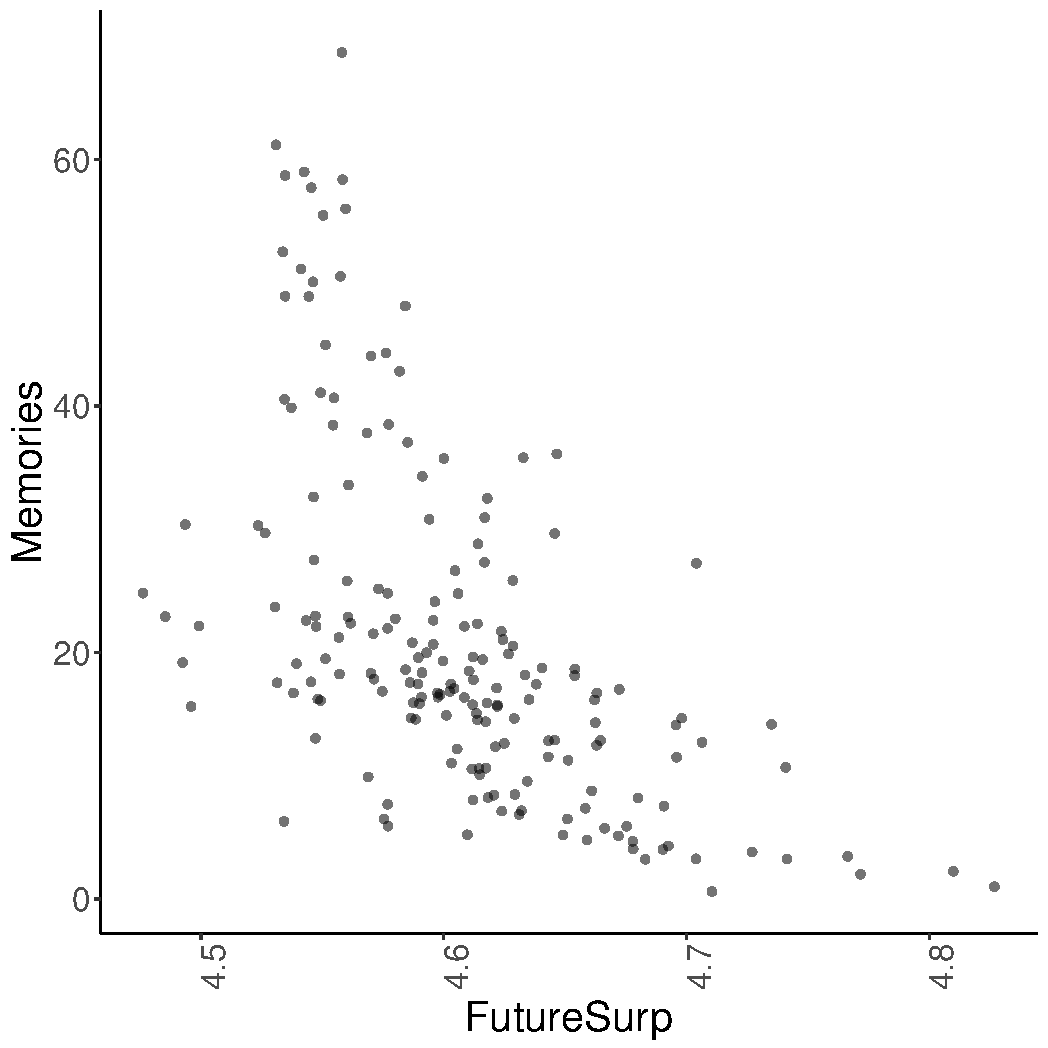
\includegraphics[width=0.3\textwidth]{code/figures/en-words-surp-mem.pdf}
%%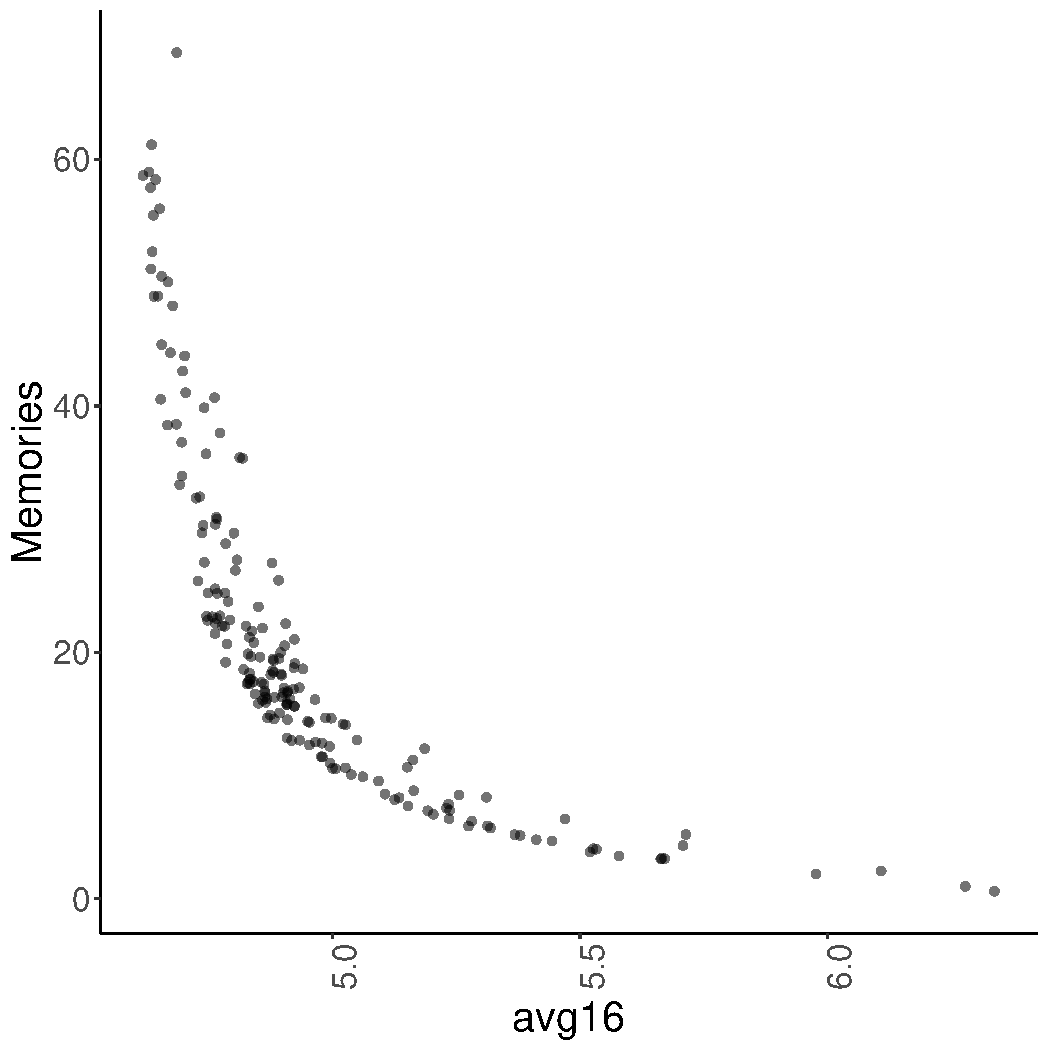
\includegraphics[width=0.3\textwidth]{code/figures/en-words-16-mem.pdf}
%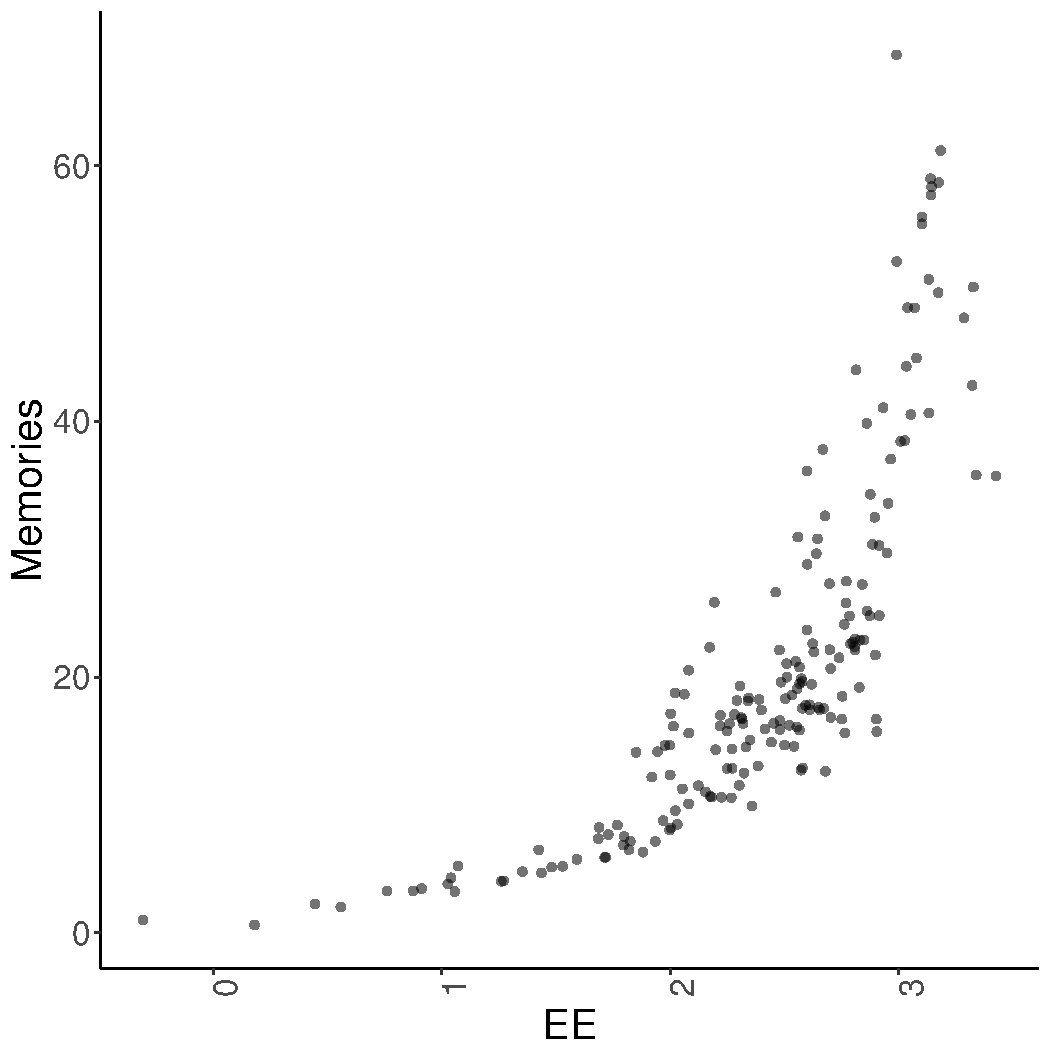
\includegraphics[width=0.3\textwidth]{code/figures/en-words-ee-mem.pdf}
%%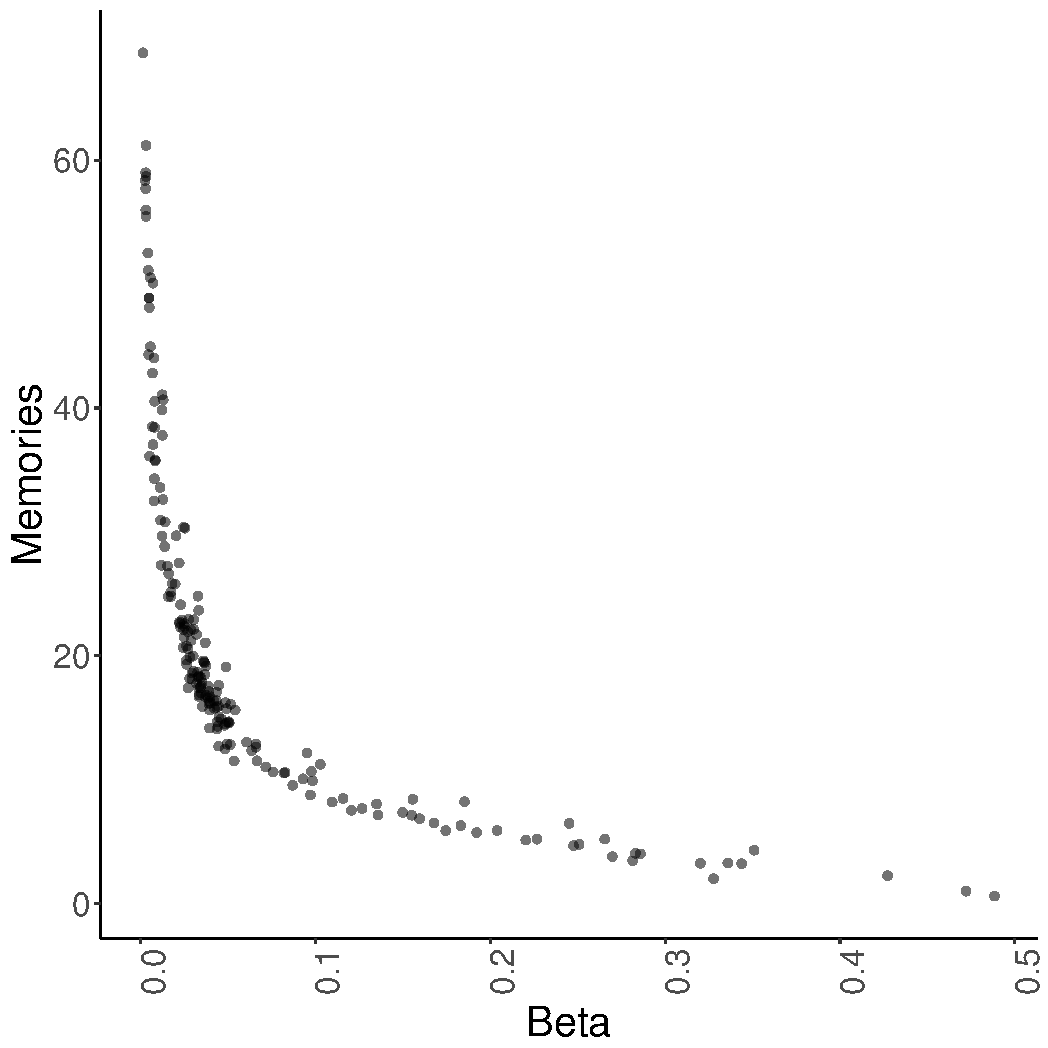
\includegraphics[width=0.3\textwidth]{code/figures/en-words-beta-mem.pdf}
%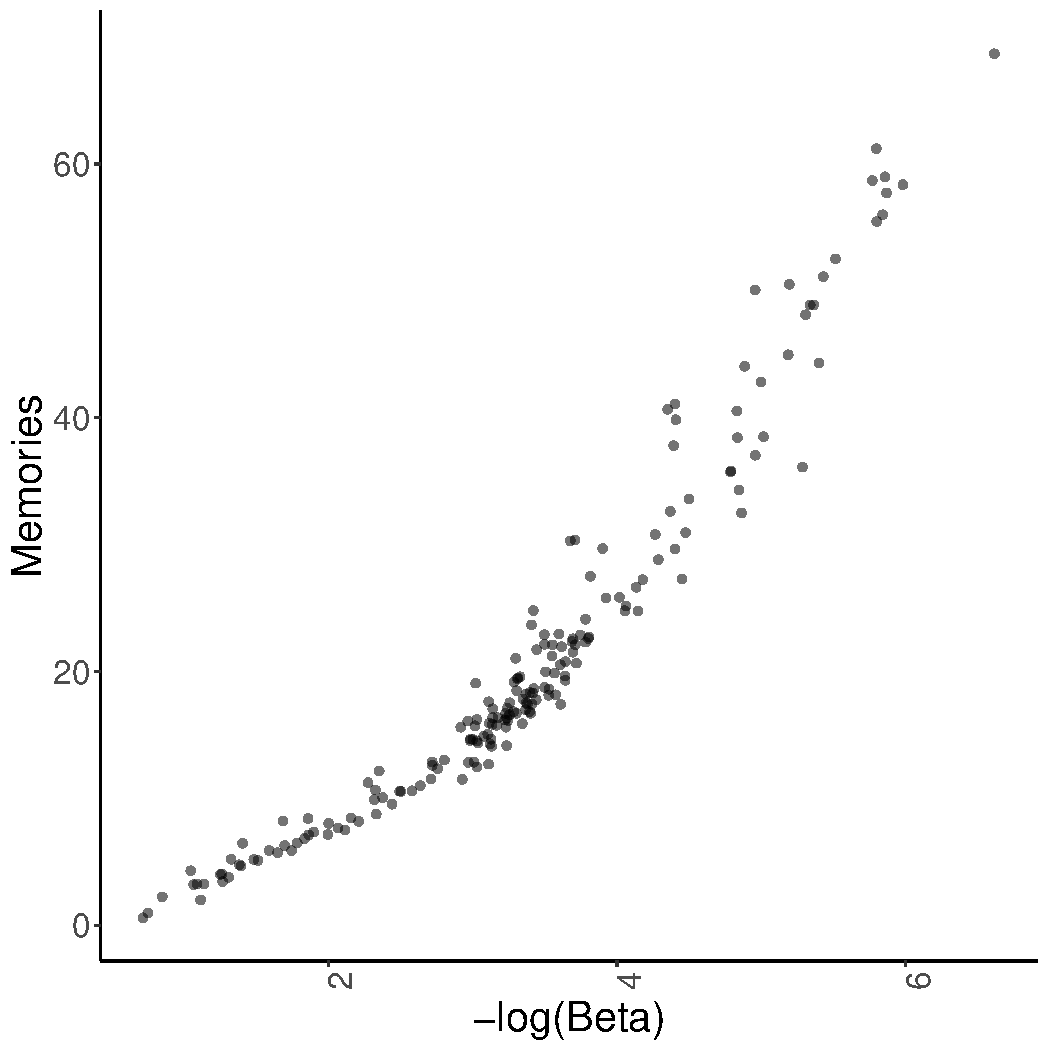
\includegraphics[width=0.3\textwidth]{code/figures/en-words-logbeta-mem.pdf}
%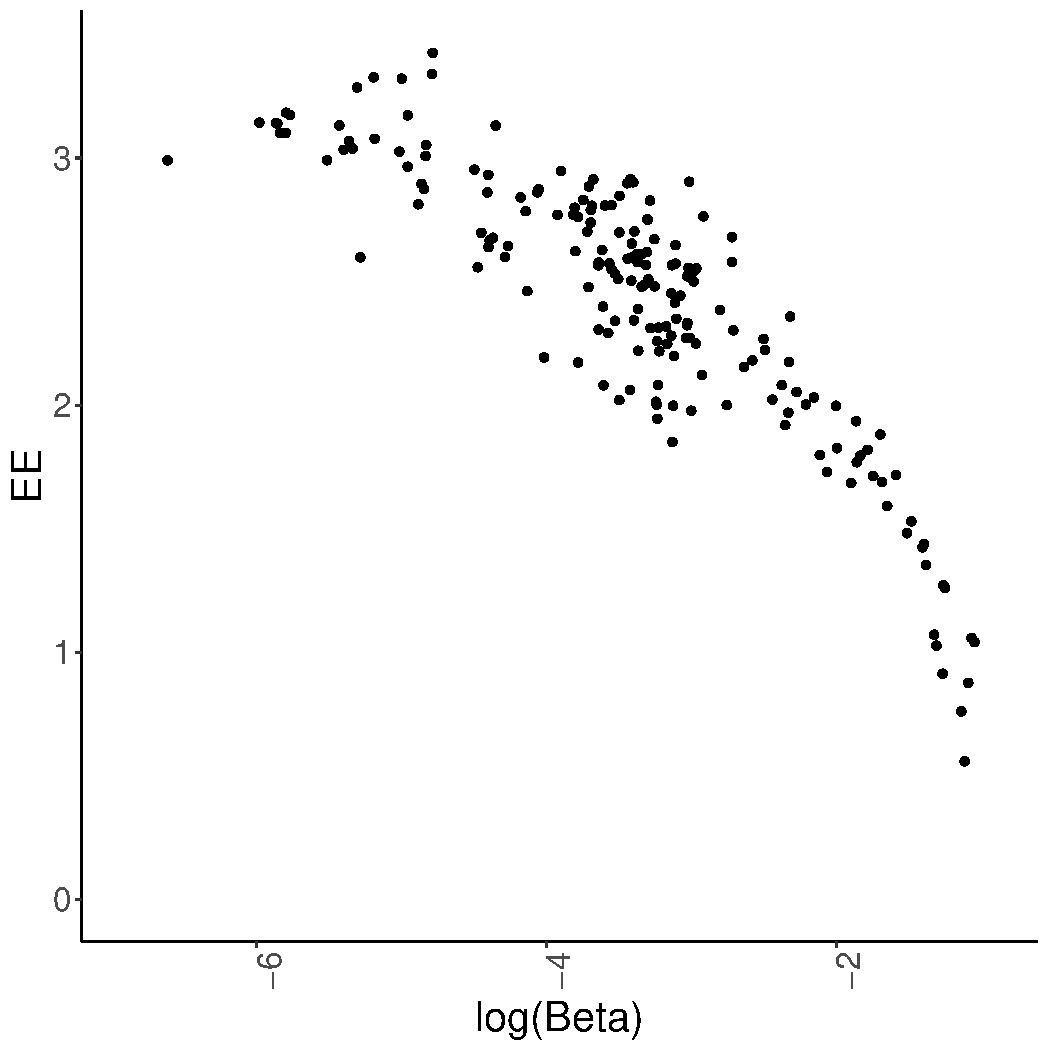
\includegraphics[width=0.3\textwidth]{code/figures/en-words-logbeta-ee.pdf}
%	\caption{Word-level modeling of English.}\label{fig:eng-logbeta}
%\end{figure*}
%
%
%
%
%\begin{figure*}
%%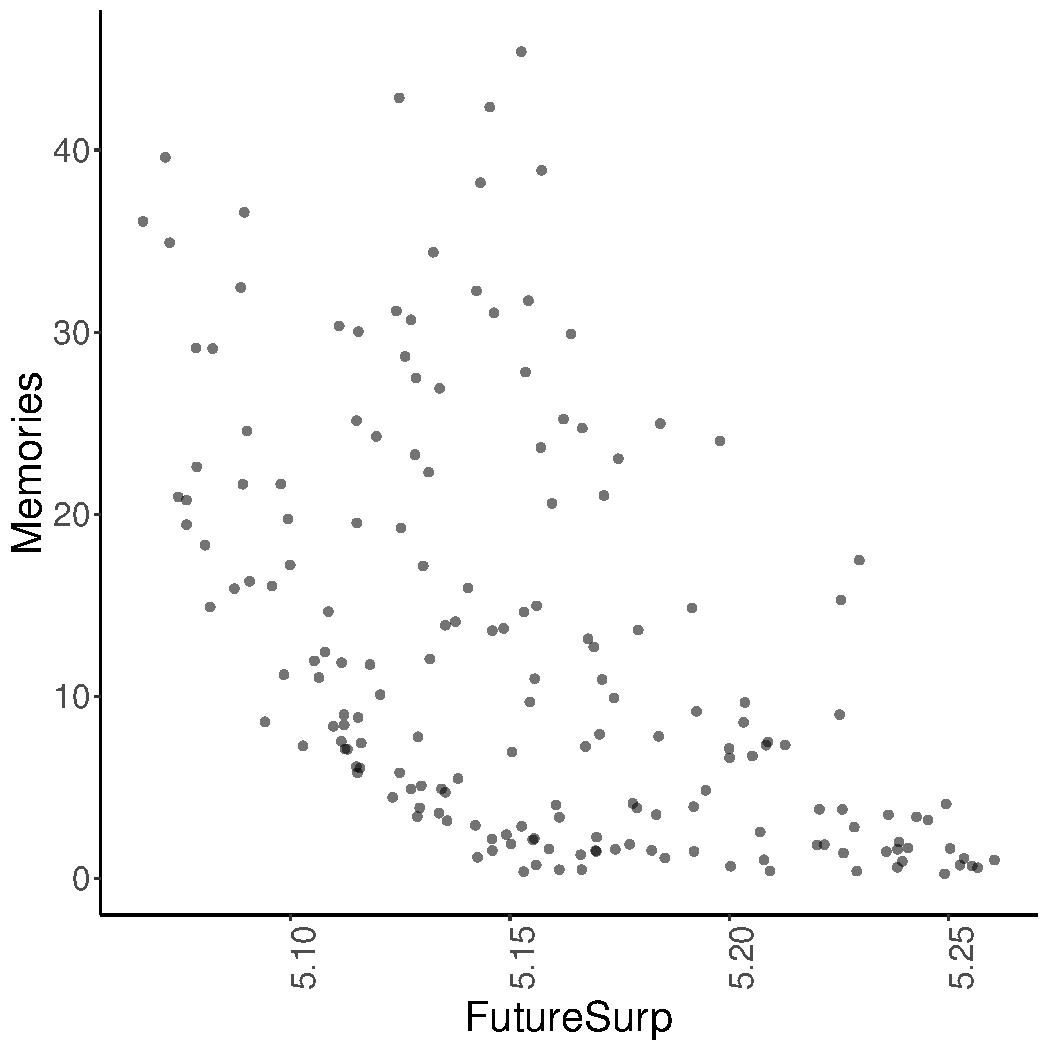
\includegraphics[width=0.3\textwidth]{code/figures/ru-words-surp-mem.pdf}
%%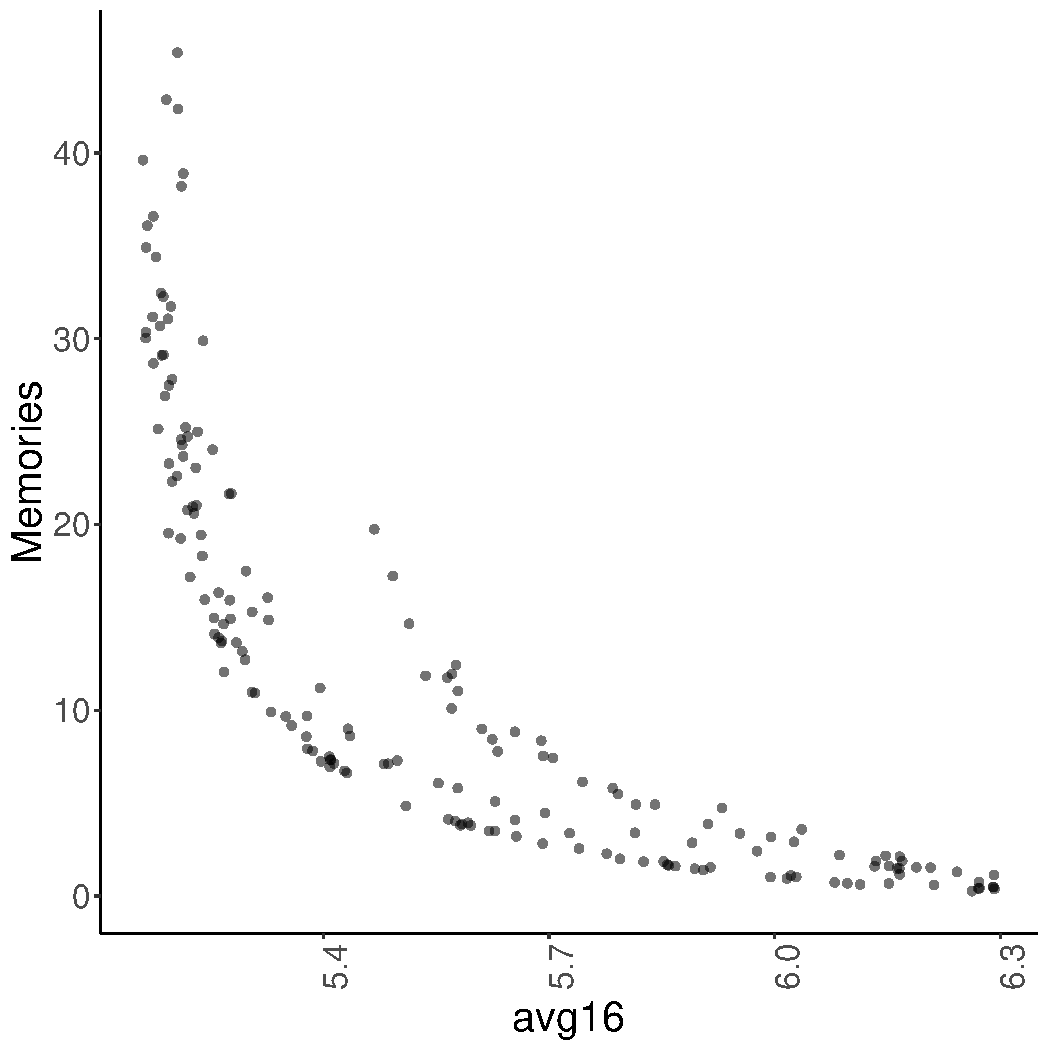
\includegraphics[width=0.3\textwidth]{code/figures/ru-words-16-mem.pdf}
%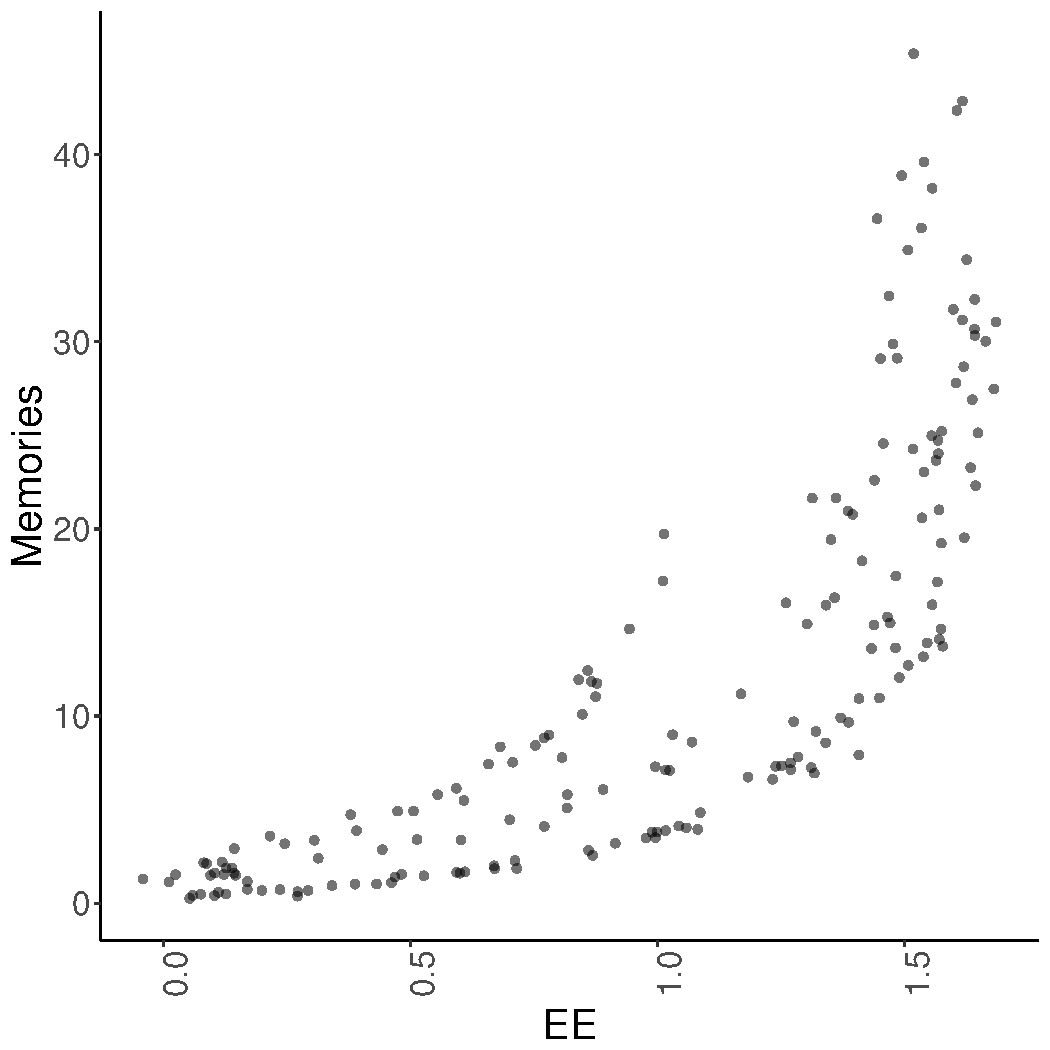
\includegraphics[width=0.3\textwidth]{code/figures/ru-words-ee-mem.pdf}
%%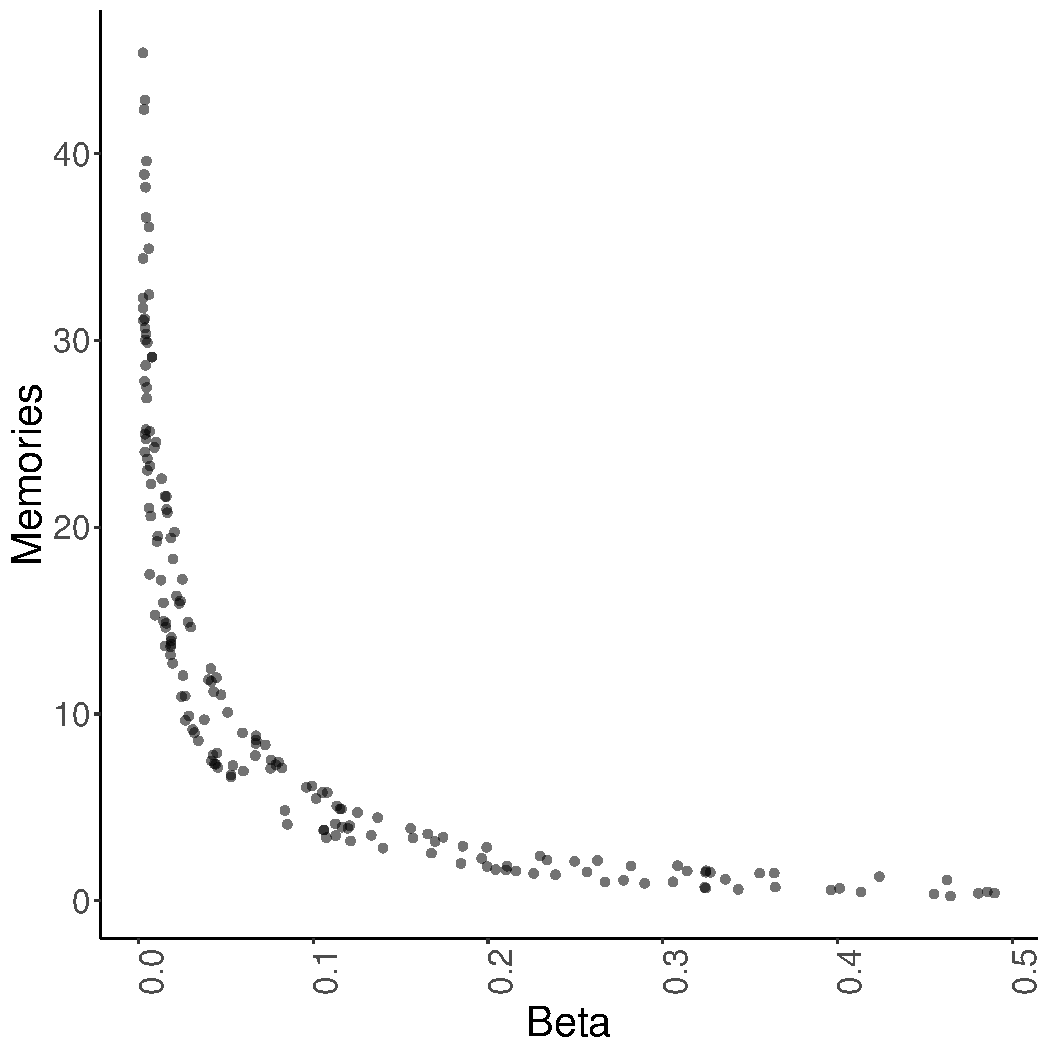
\includegraphics[width=0.3\textwidth]{code/figures/ru-words-beta-mem.pdf}
%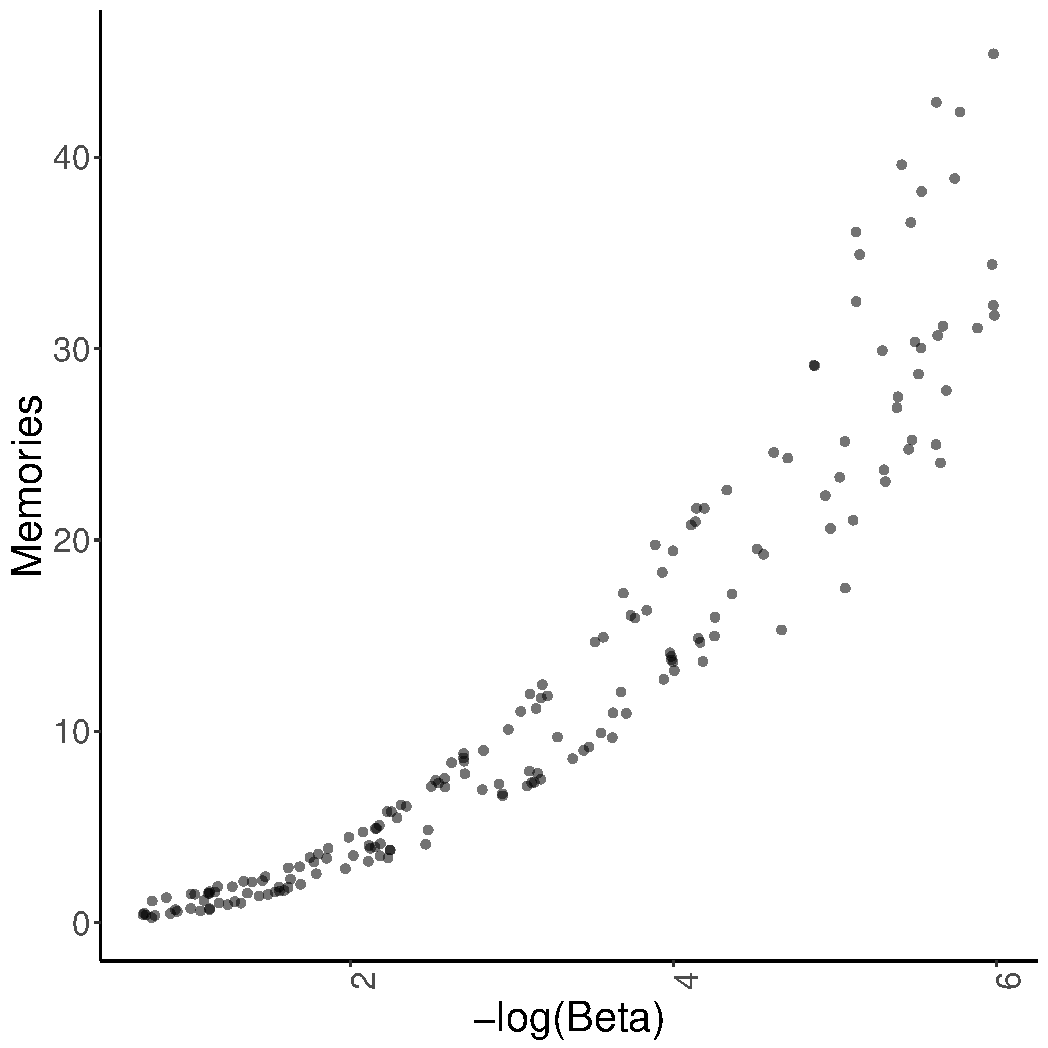
\includegraphics[width=0.3\textwidth]{code/figures/ru-words-logbeta-mem.pdf}
%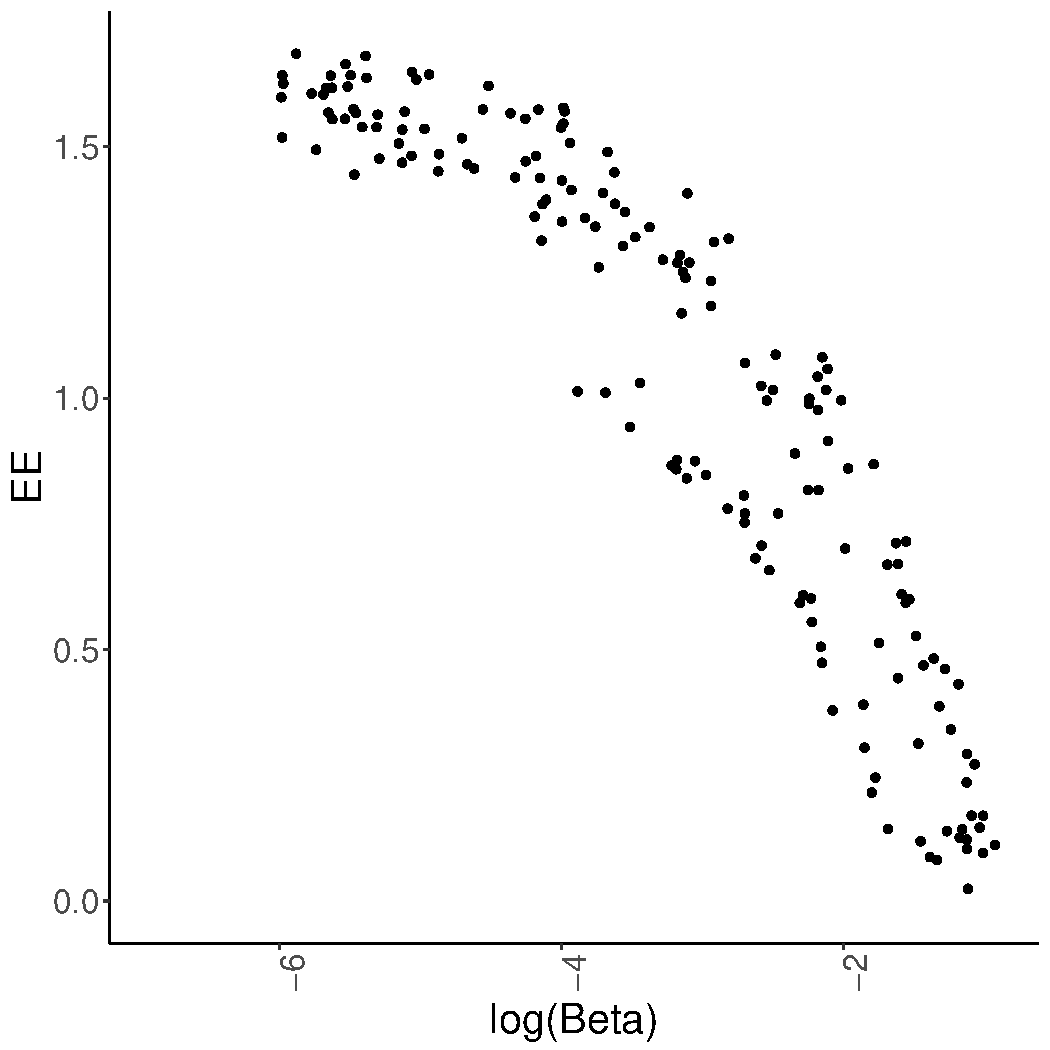
\includegraphics[width=0.3\textwidth]{code/figures/ru-words-logbeta-ee.pdf}
%	\caption{Word-level modeling of Russian.}\label{fig:rug-logbeta}
%\end{figure*}
%
%
%
%\begin{figure*}
%%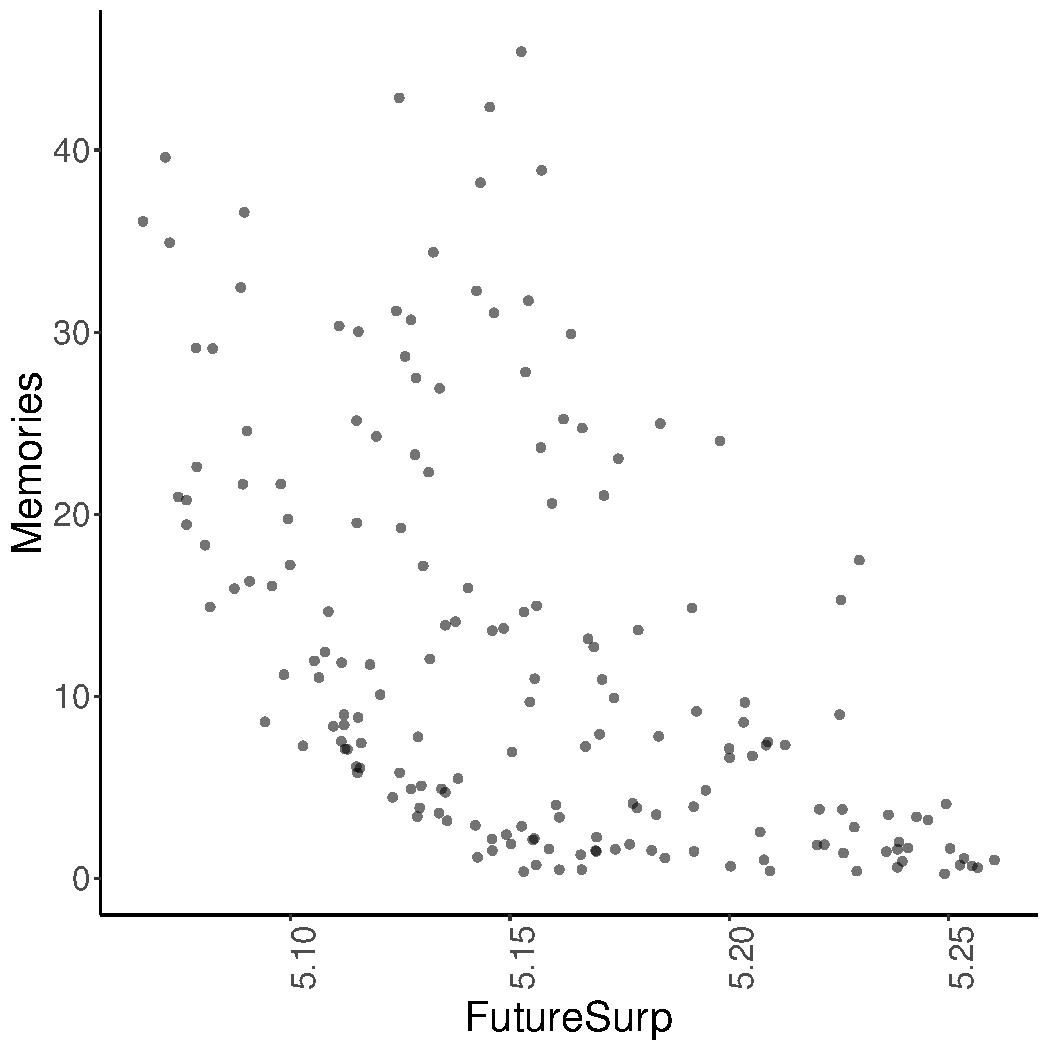
\includegraphics[width=0.3\textwidth]{code/figures/ru-words-surp-mem.pdf}
%%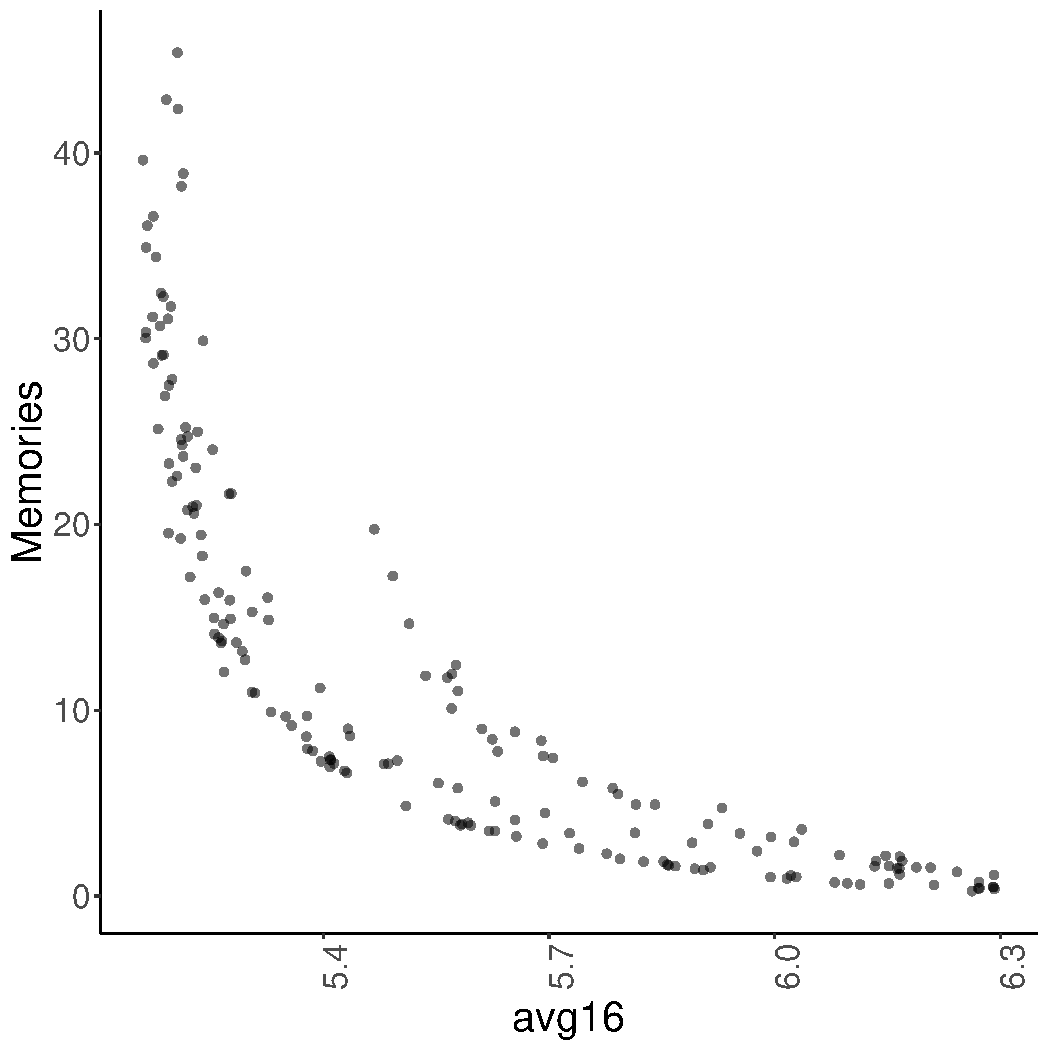
\includegraphics[width=0.3\textwidth]{code/figures/ru-words-16-mem.pdf}
%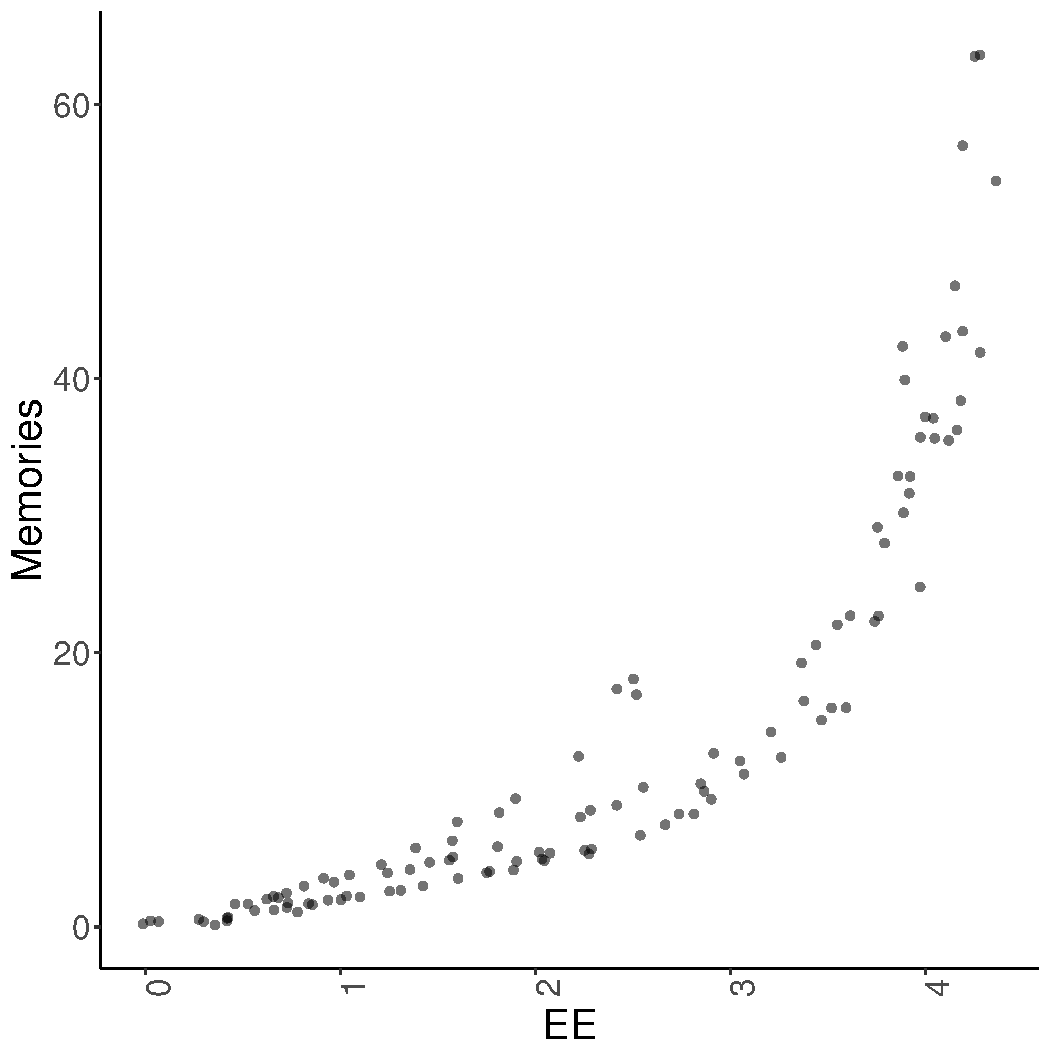
\includegraphics[width=0.3\textwidth]{code/figures/LDC95T8-words-ee-mem.pdf}
%%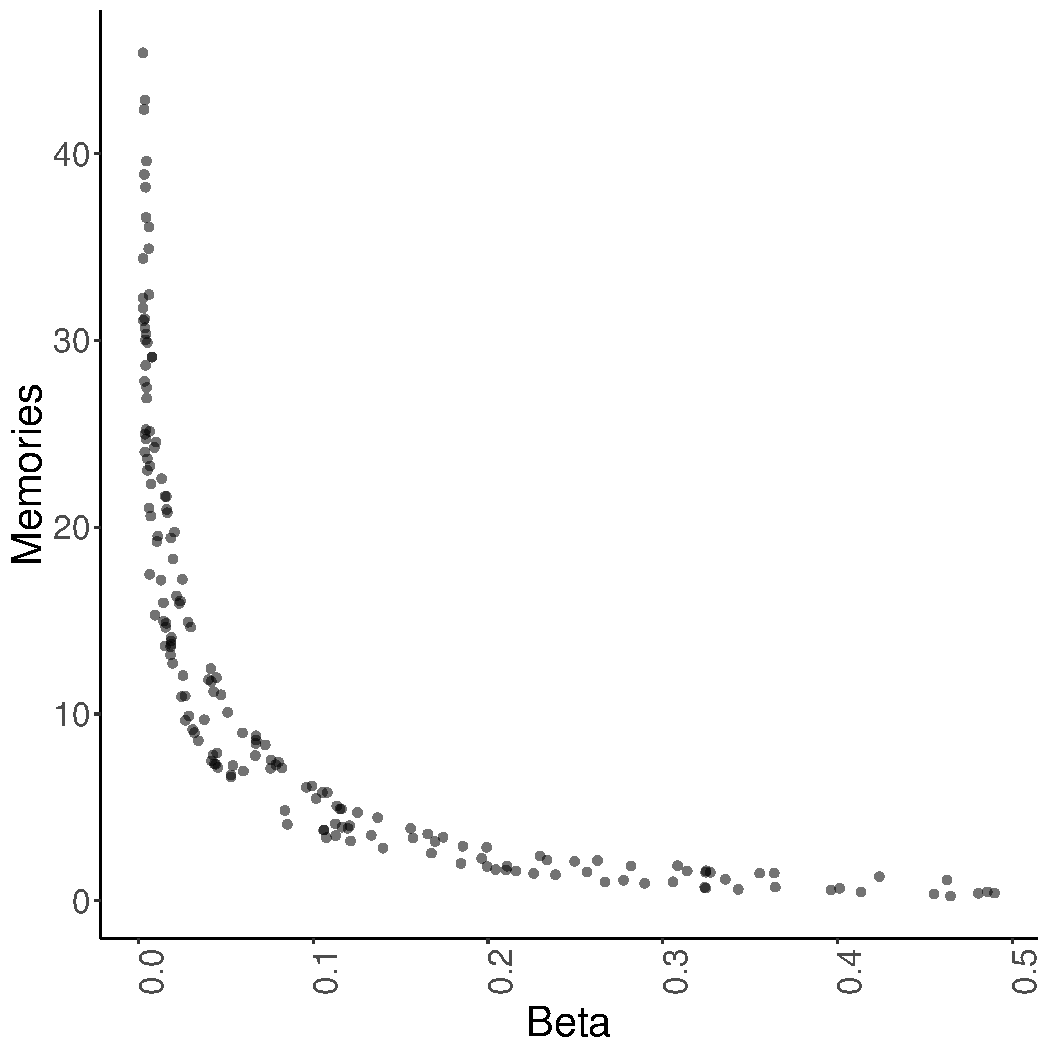
\includegraphics[width=0.3\textwidth]{code/figures/ru-words-beta-mem.pdf}
%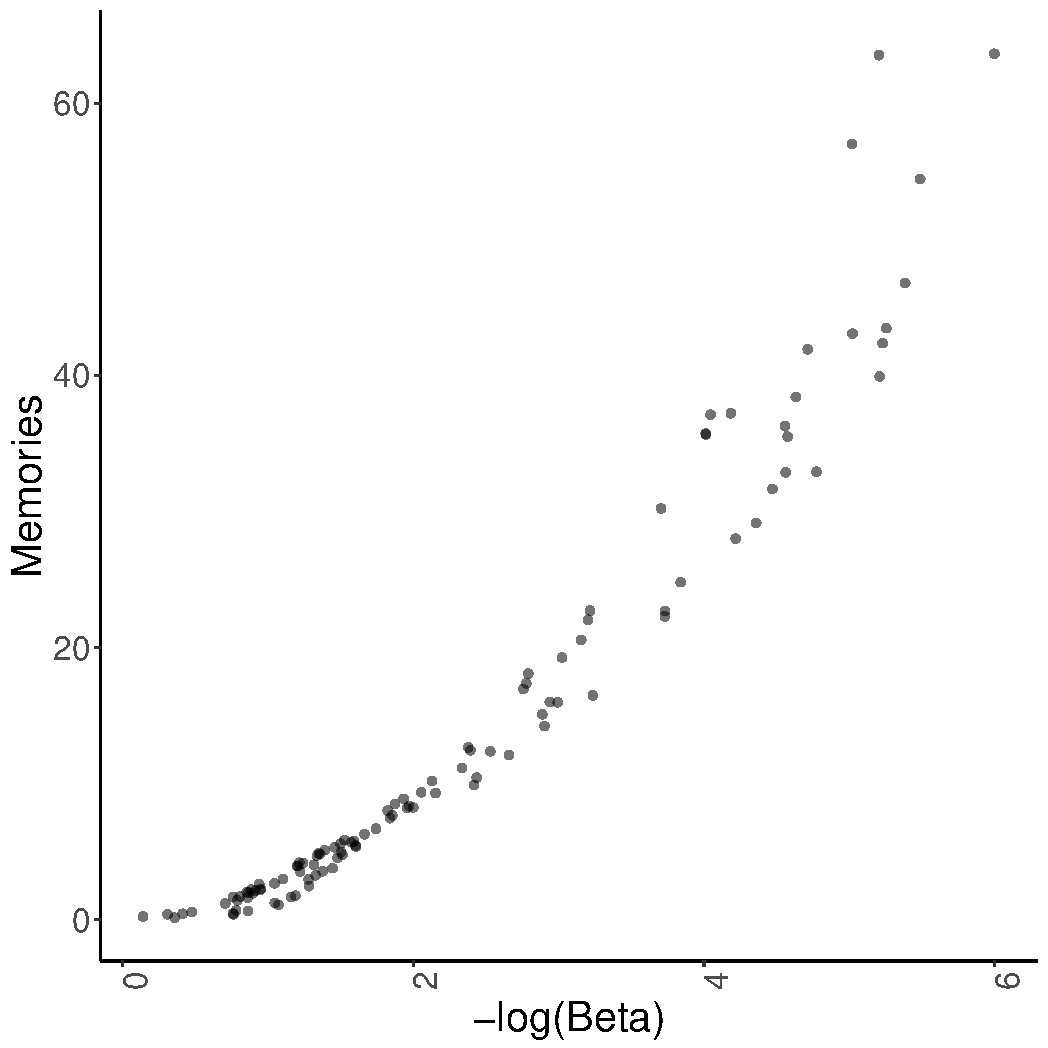
\includegraphics[width=0.3\textwidth]{code/figures/LDC95T8-words-logbeta-mem.pdf}
%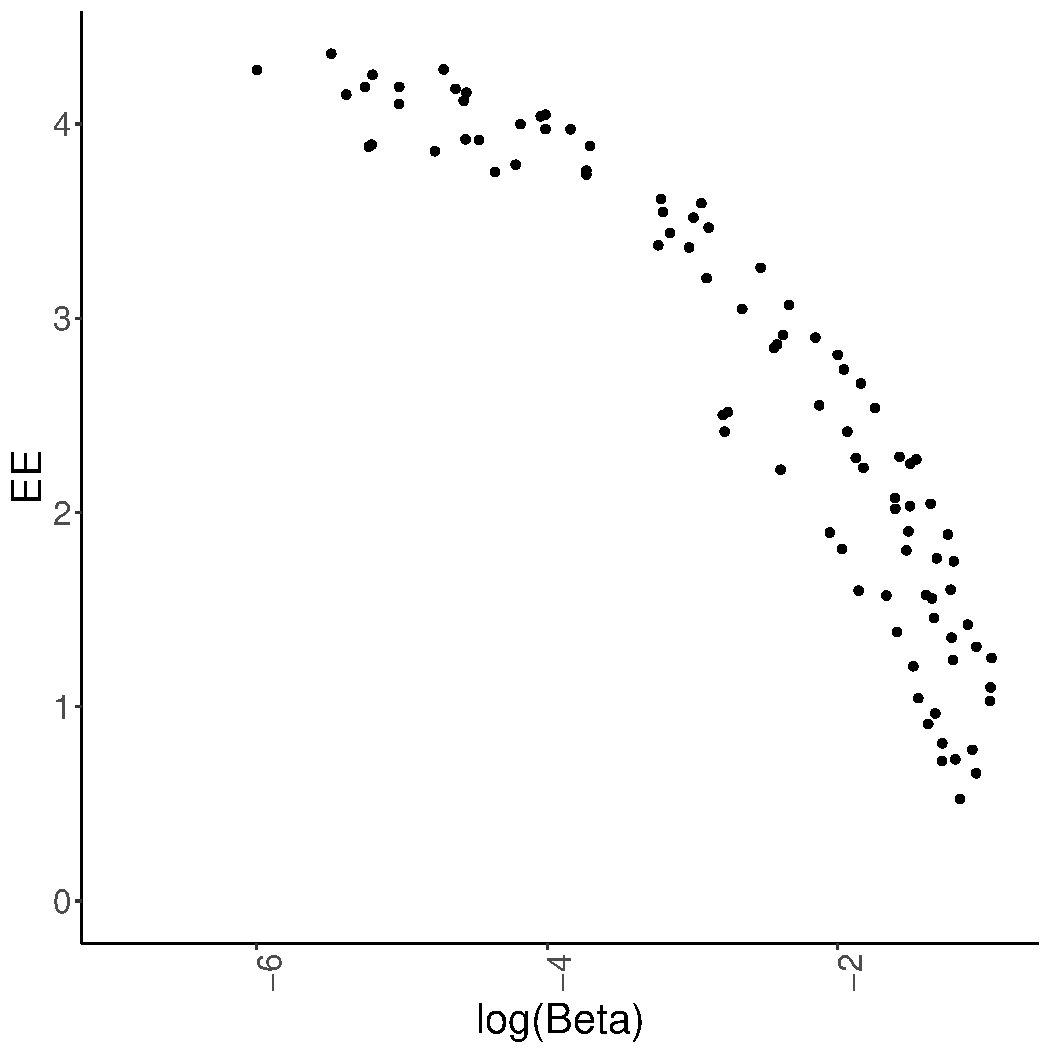
\includegraphics[width=0.3\textwidth]{code/figures/LDC95T8-words-logbeta-ee.pdf}
%	\caption{Word-level modeling of Japanese.}\label{fig:jap-logbeta}
%\end{figure*}
%
%
%
%\begin{figure*}
%%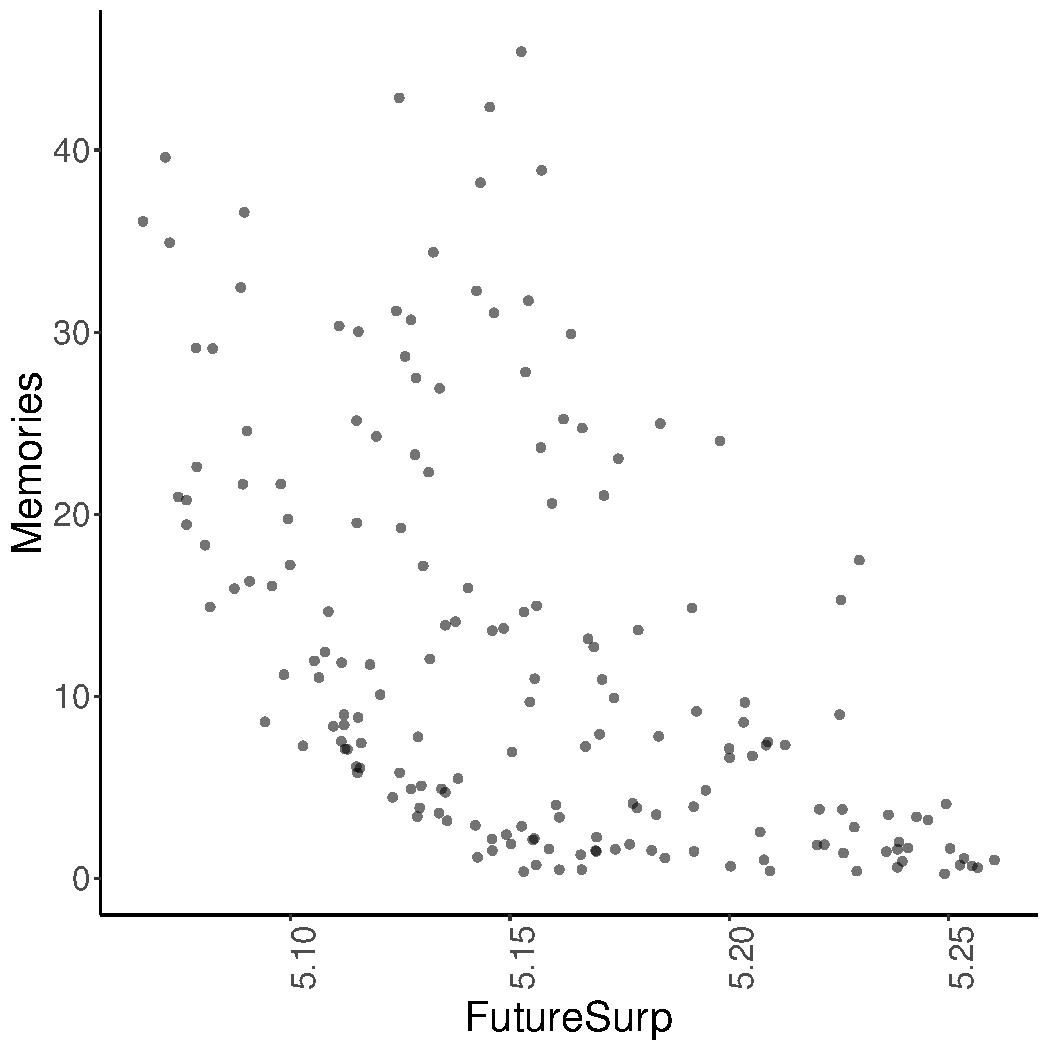
\includegraphics[width=0.3\textwidth]{code/figures/ru-words-surp-mem.pdf}
%%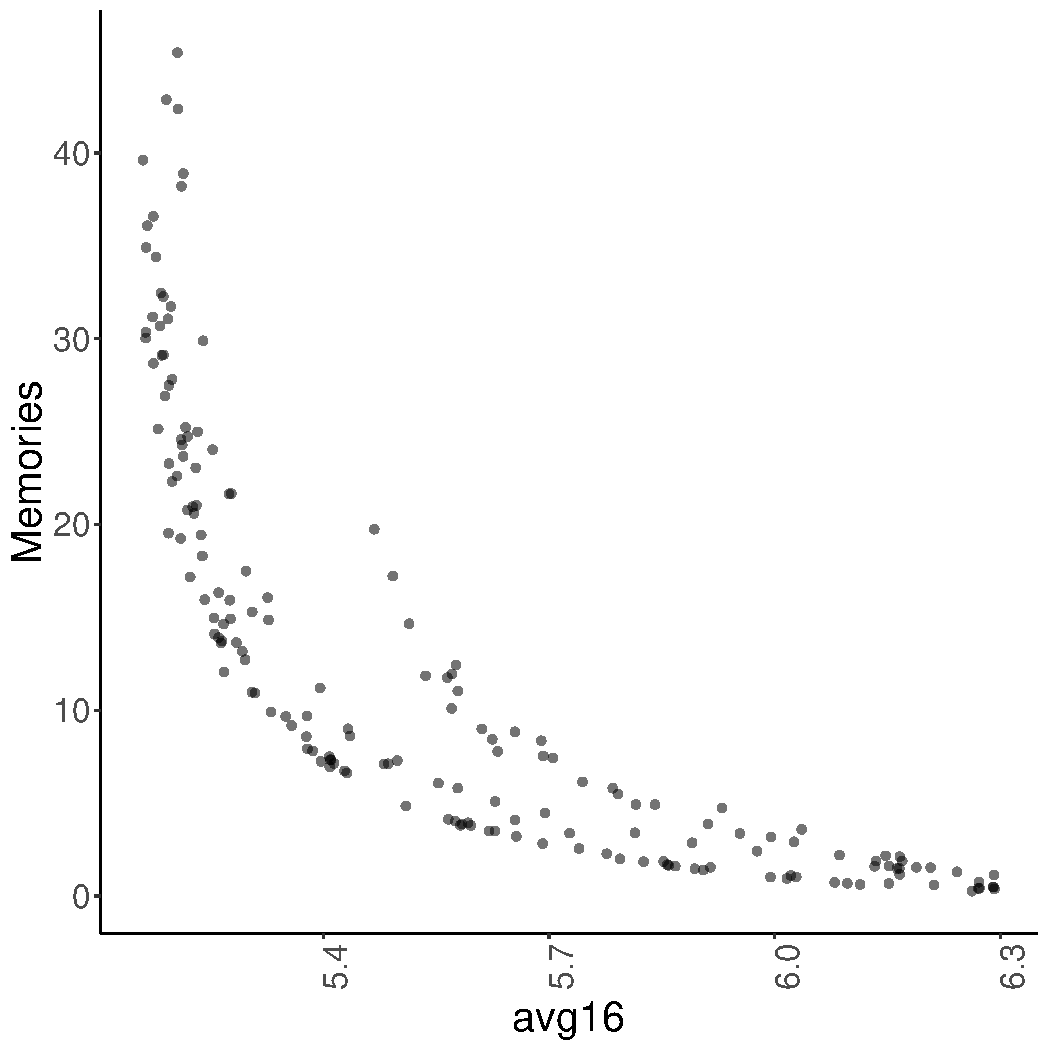
\includegraphics[width=0.3\textwidth]{code/figures/ru-words-16-mem.pdf}
%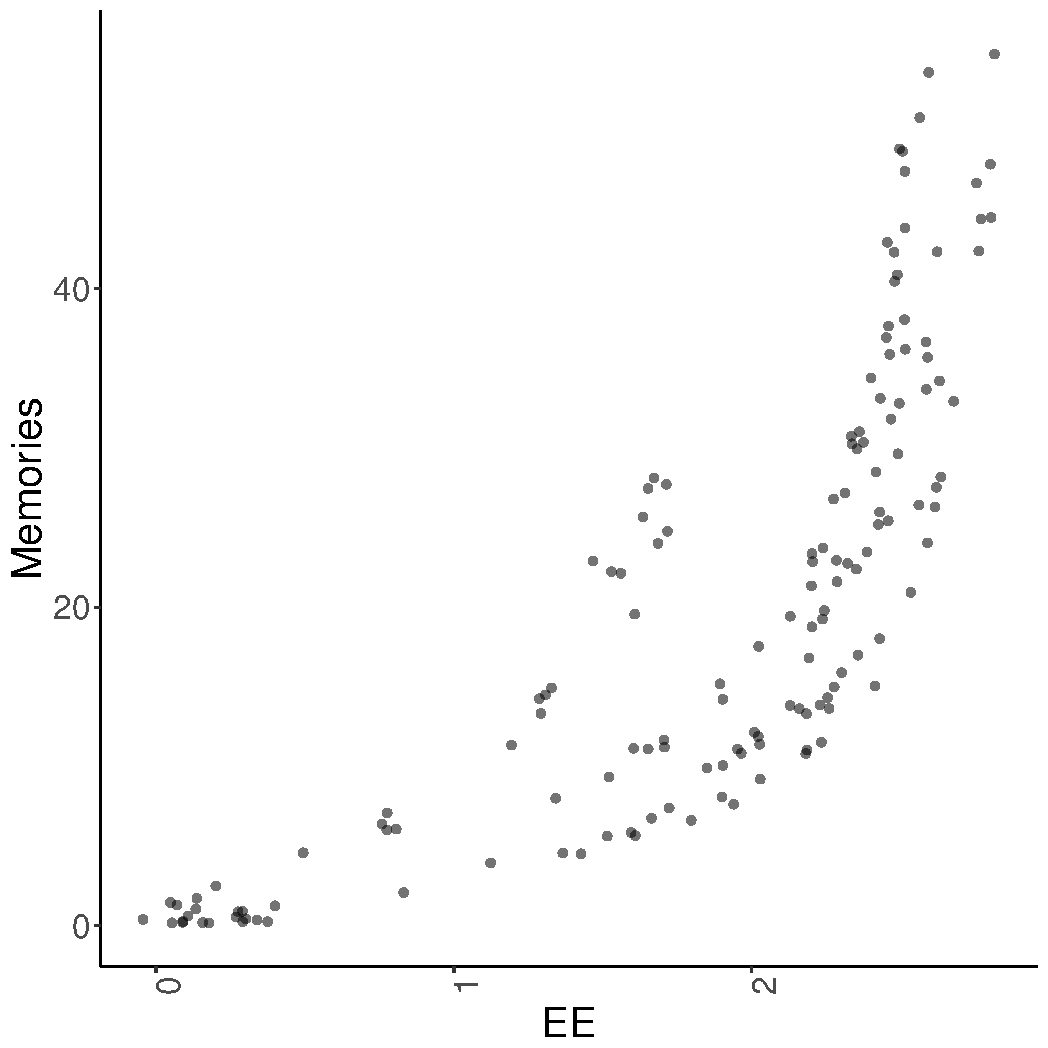
\includegraphics[width=0.3\textwidth]{code/figures/LDC2012T05-words-ee-mem.pdf}
%%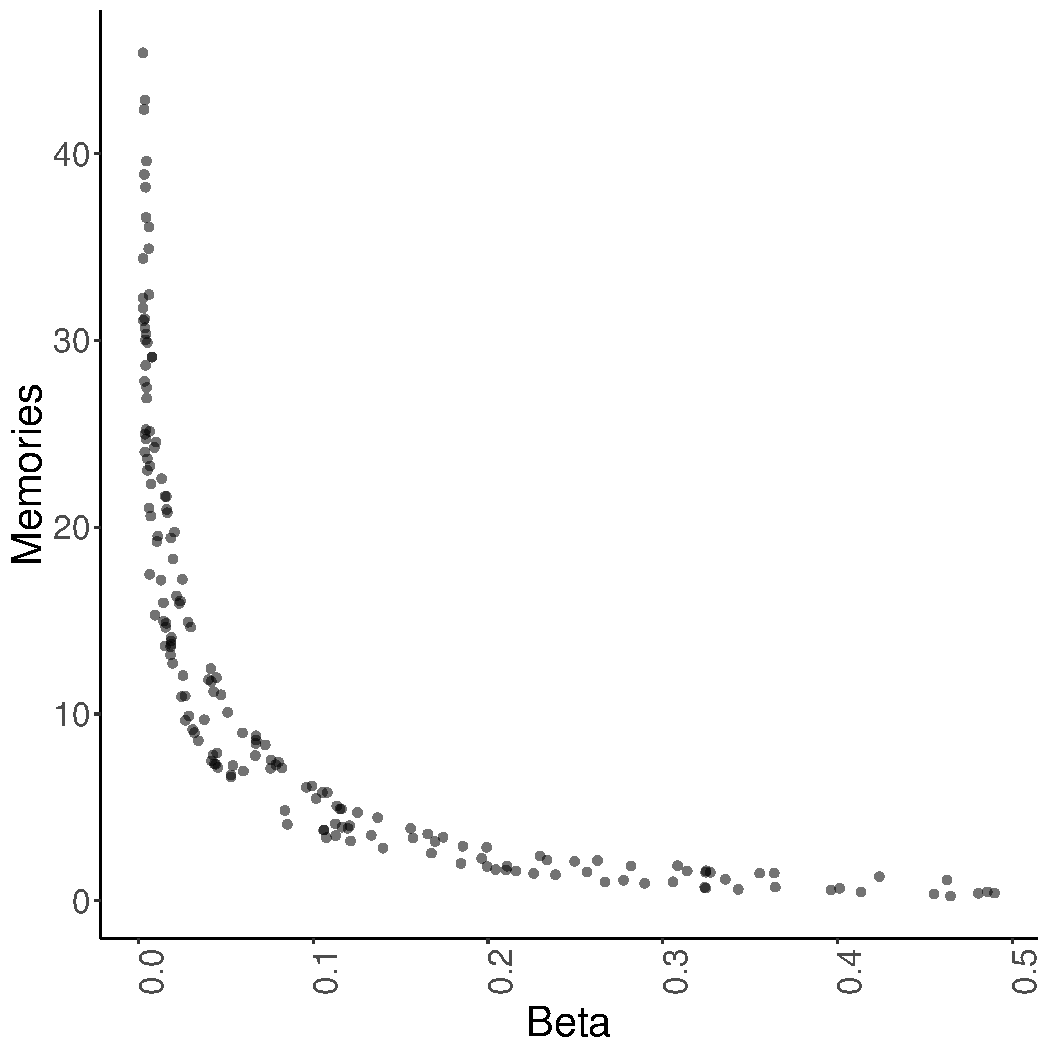
\includegraphics[width=0.3\textwidth]{code/figures/ru-words-beta-mem.pdf}
%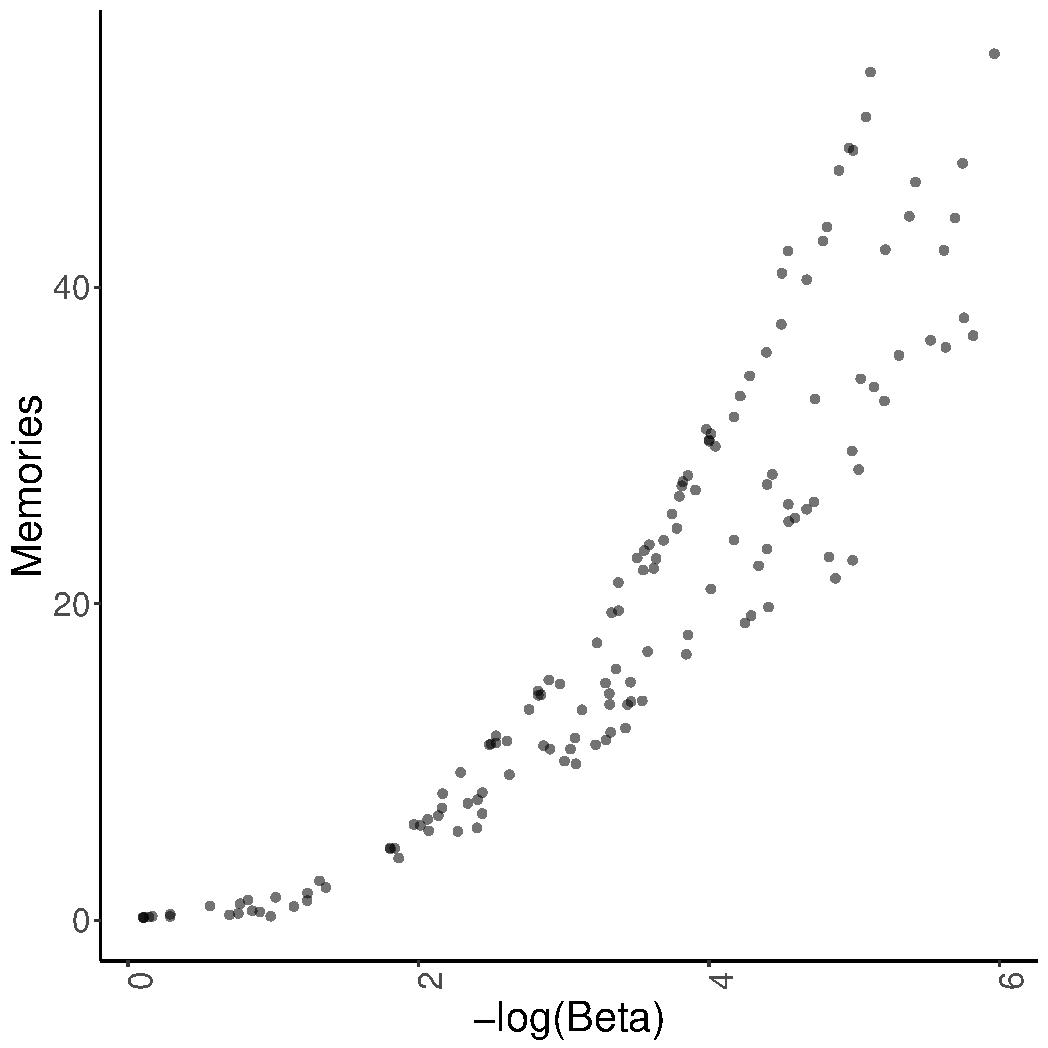
\includegraphics[width=0.3\textwidth]{code/figures/LDC2012T05-words-logbeta-mem.pdf}
%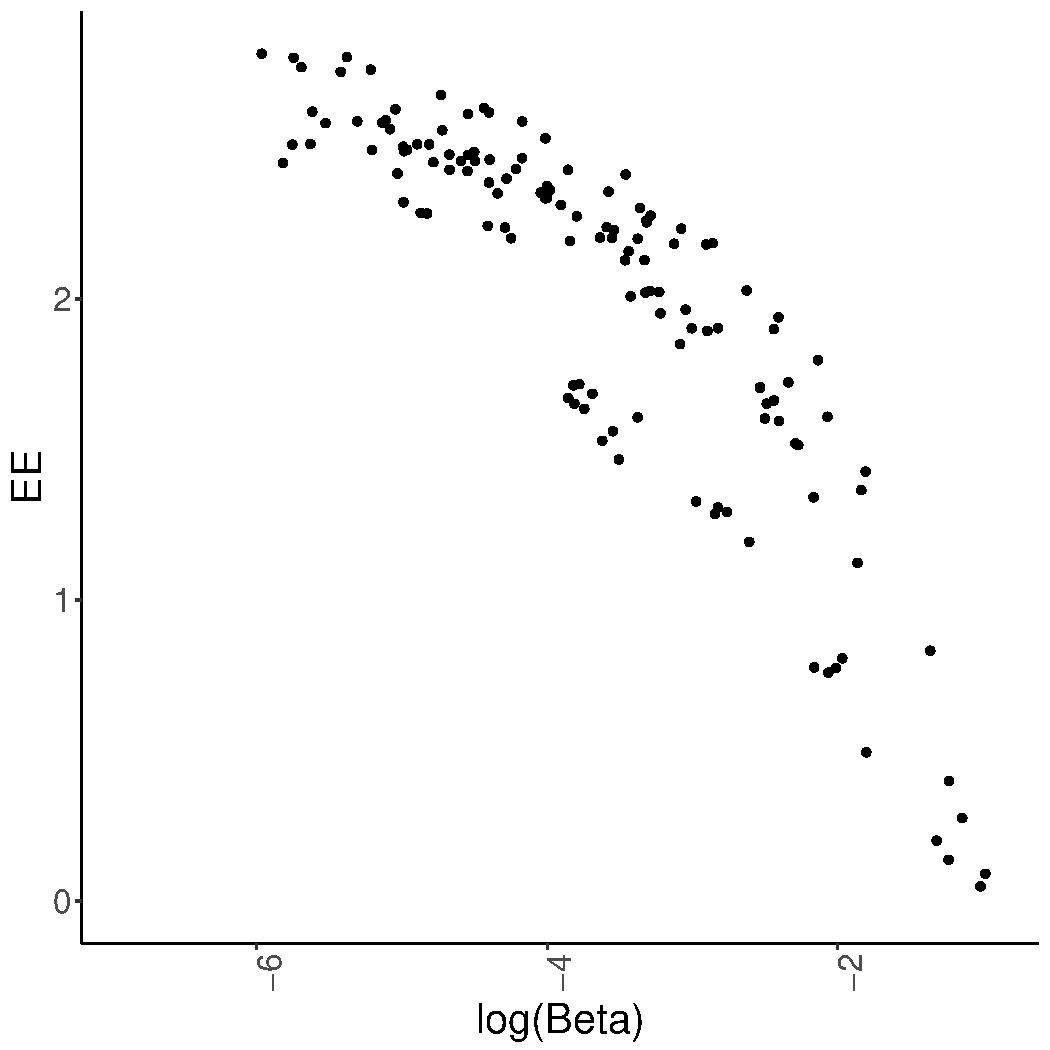
\includegraphics[width=0.3\textwidth]{code/figures/LDC2012T05-words-logbeta-ee.pdf}
%	\caption{Word-level modeling of Chinese.}\label{fig:jap-logbeta}
%\end{figure*}
%
%
%
%\begin{figure*}
%%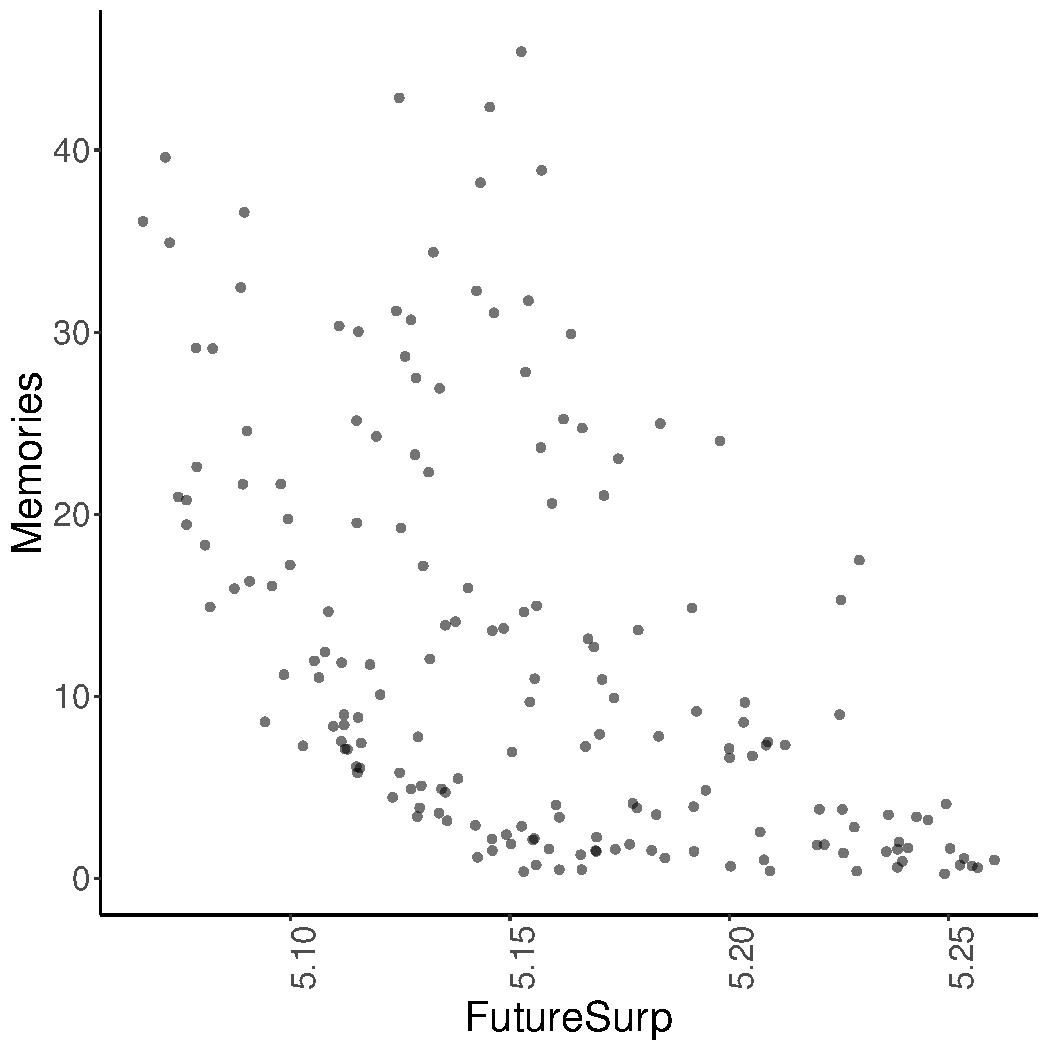
\includegraphics[width=0.3\textwidth]{code/figures/ru-words-surp-mem.pdf}
%%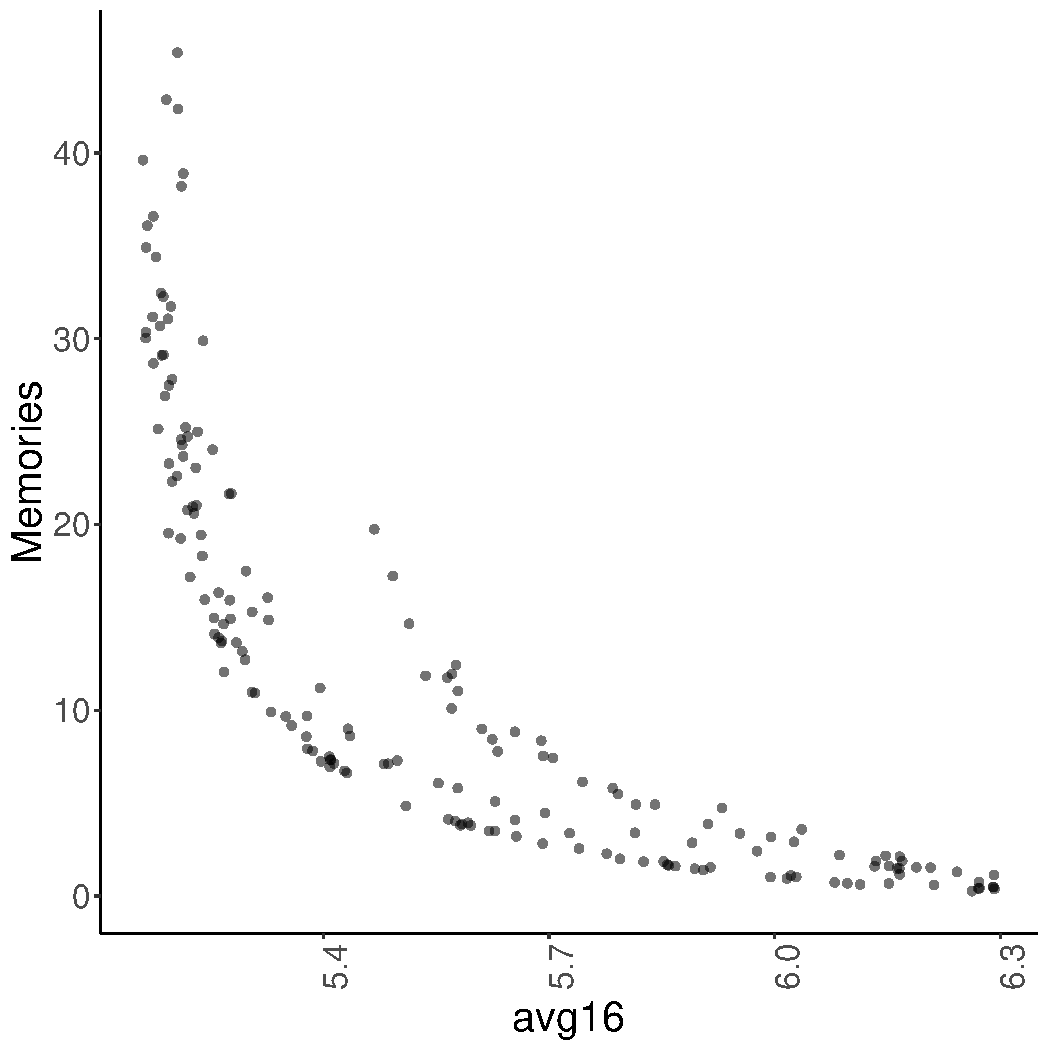
\includegraphics[width=0.3\textwidth]{code/figures/ru-words-16-mem.pdf}
%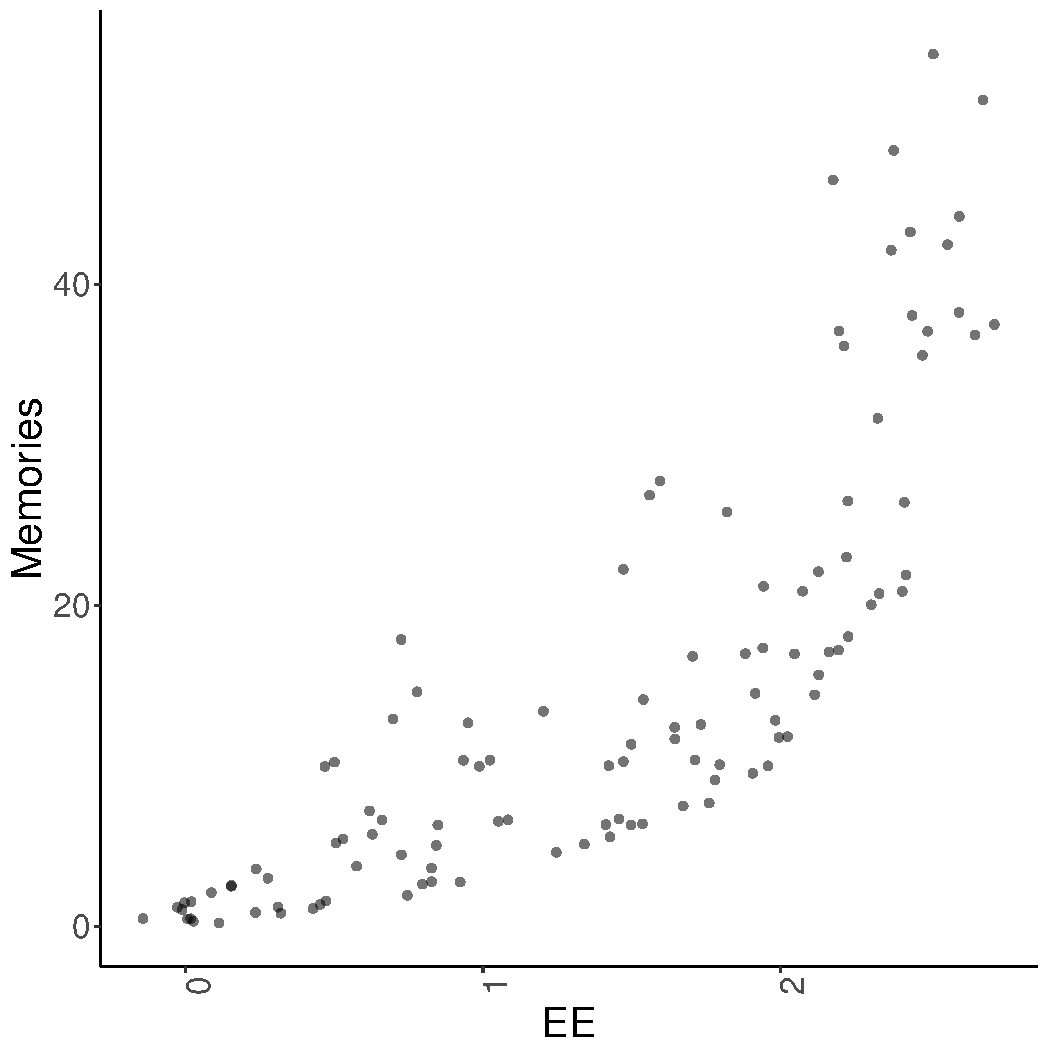
\includegraphics[width=0.3\textwidth]{code/figures/ar-words-ee-mem.pdf}
%%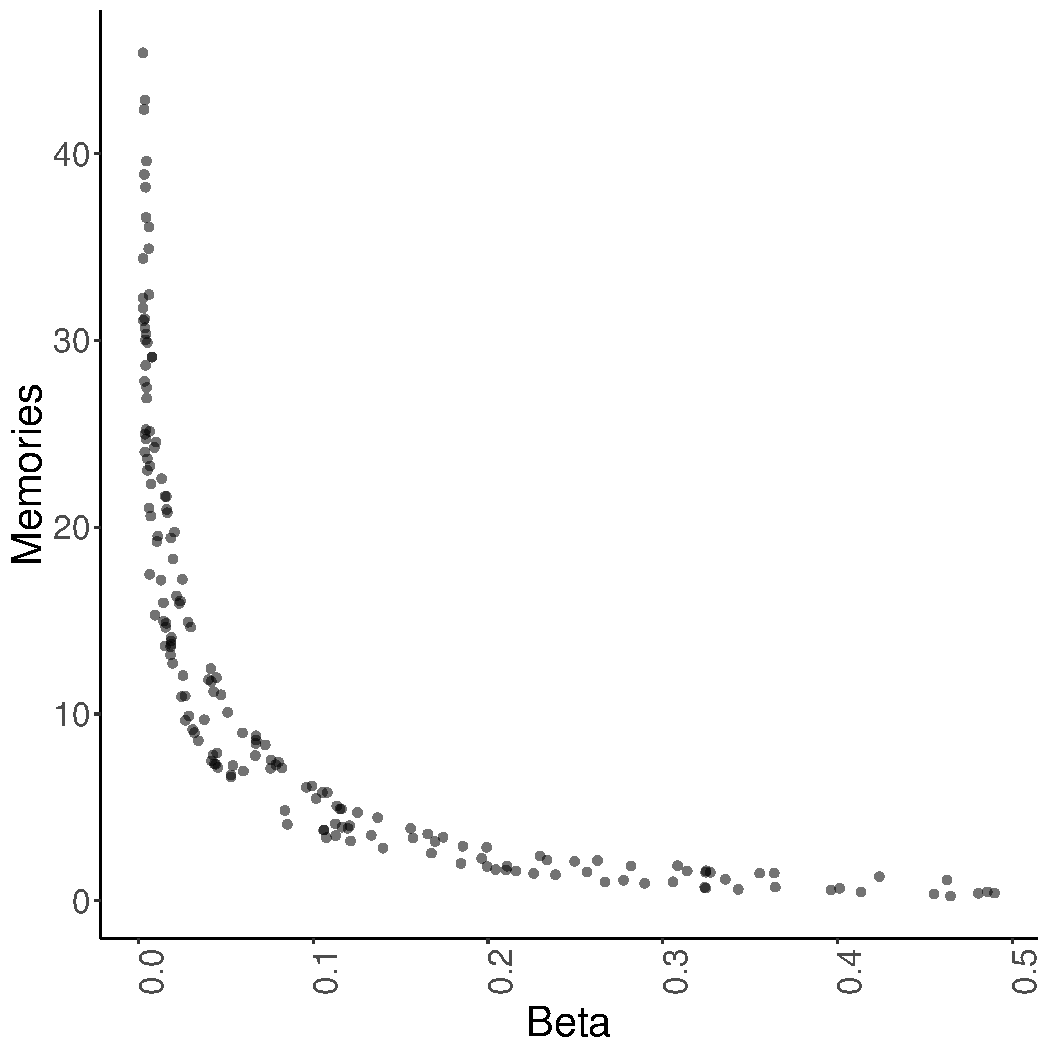
\includegraphics[width=0.3\textwidth]{code/figures/ru-words-beta-mem.pdf}
%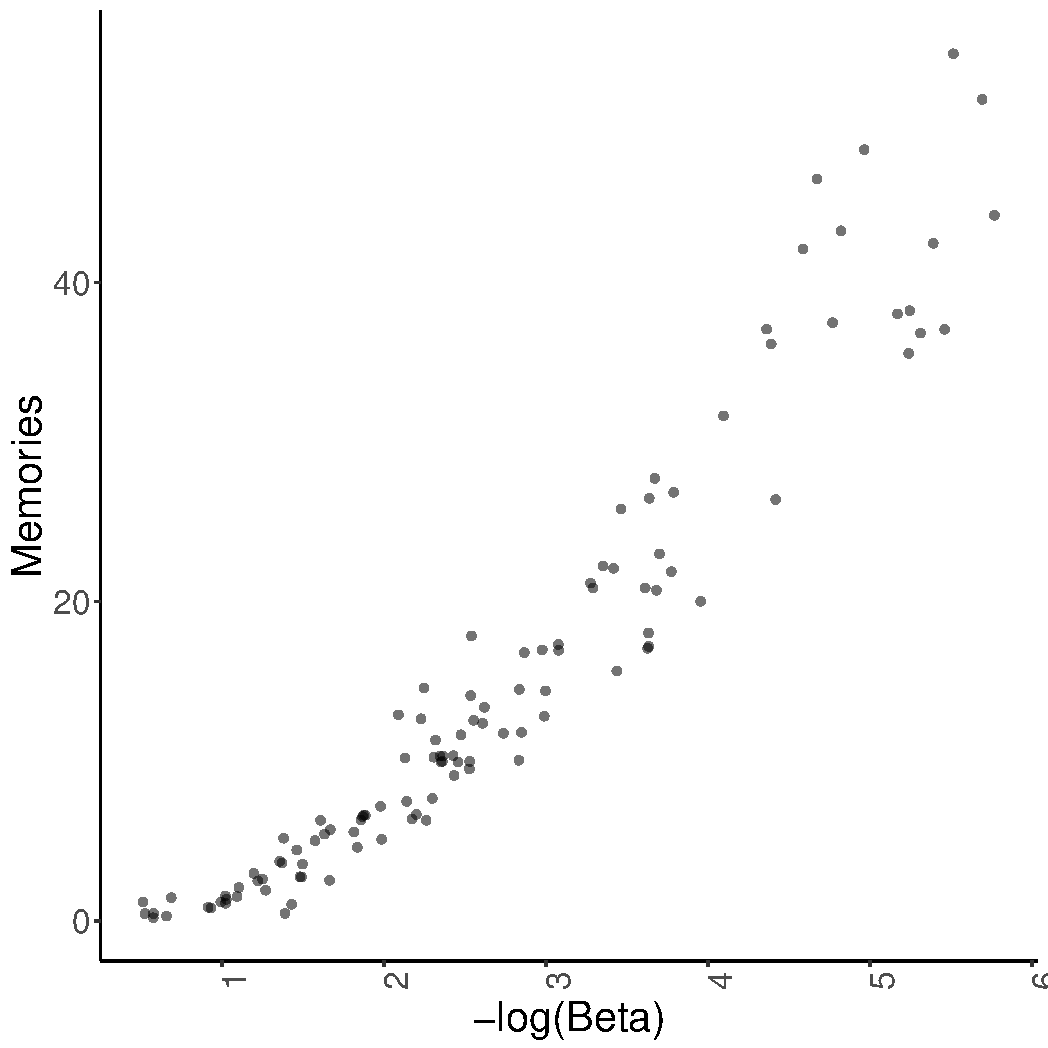
\includegraphics[width=0.3\textwidth]{code/figures/ar-words-logbeta-mem.pdf}
%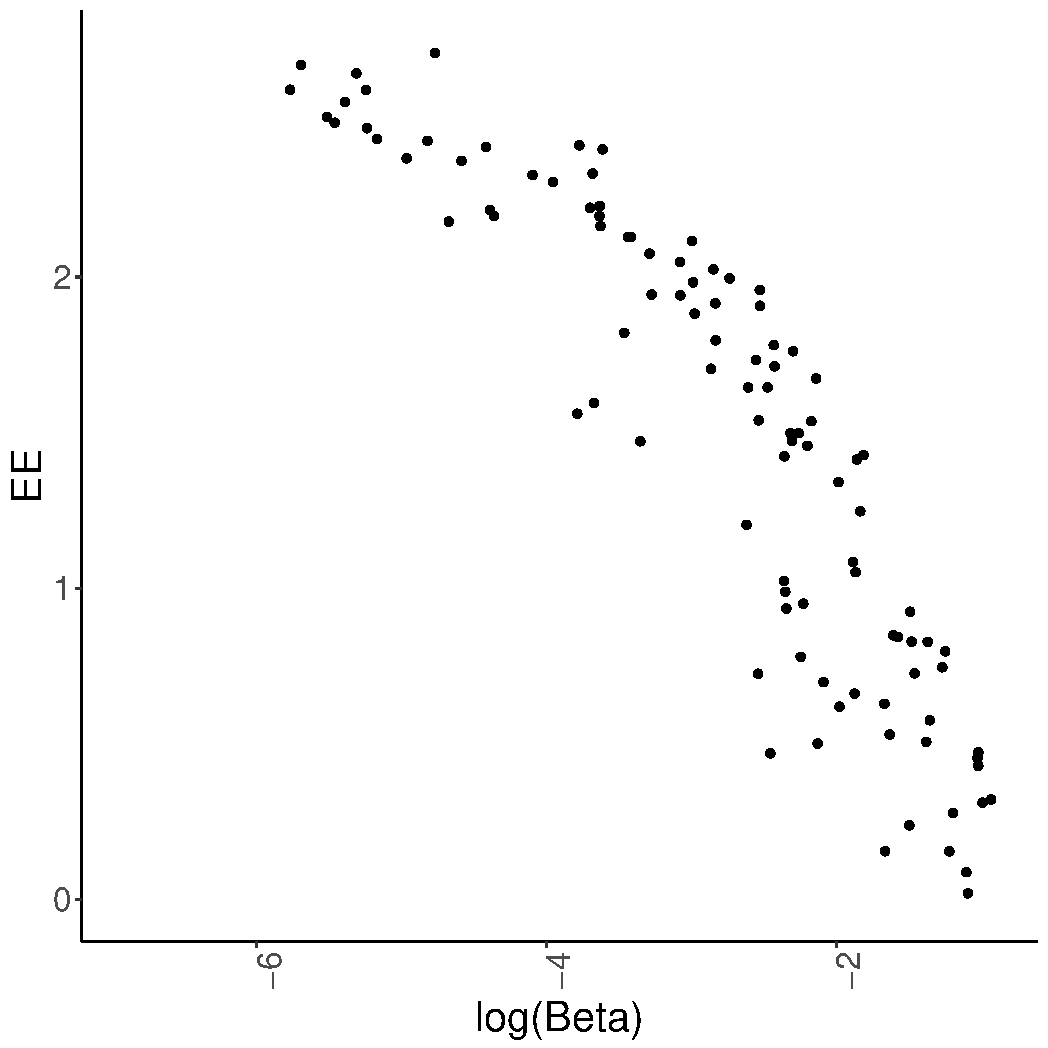
\includegraphics[width=0.3\textwidth]{code/figures/ar-words-logbeta-ee.pdf}
%	\caption{Word-level modeling of Arabic.}\label{fig:jap-logbeta}
%\end{figure*}
%
%
%
%
%
%
%\begin{figure*}
%%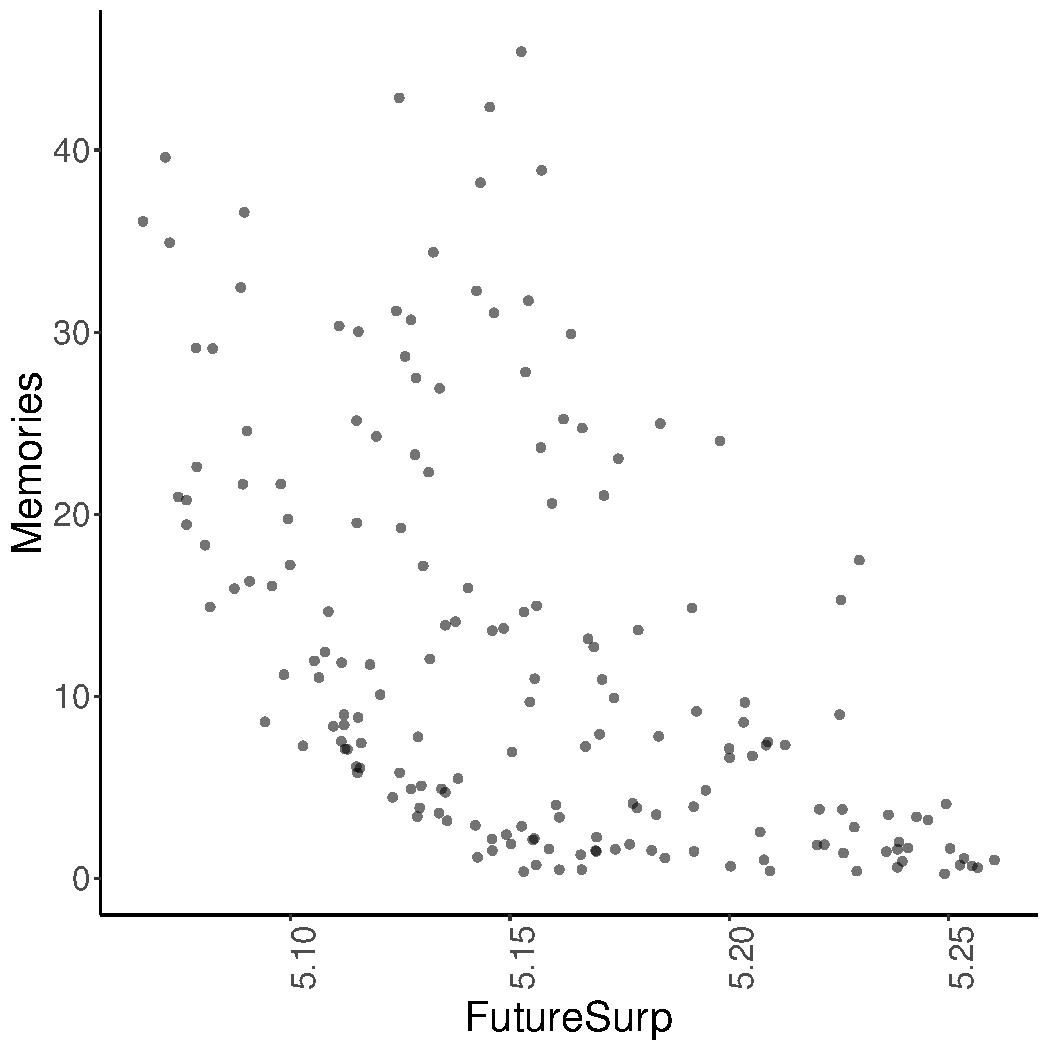
\includegraphics[width=0.3\textwidth]{code/figures/ru-words-surp-mem.pdf}
%%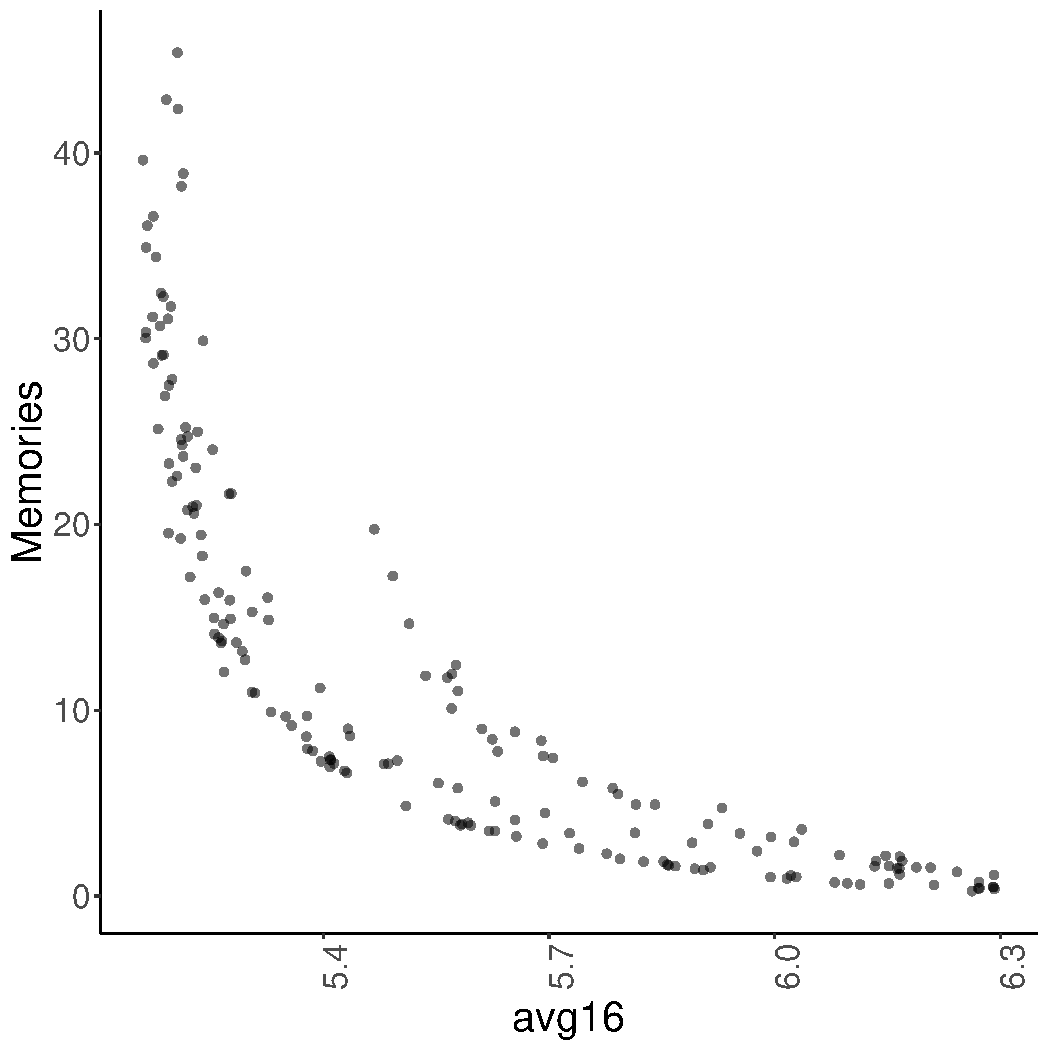
\includegraphics[width=0.3\textwidth]{code/figures/ru-words-16-mem.pdf}
%%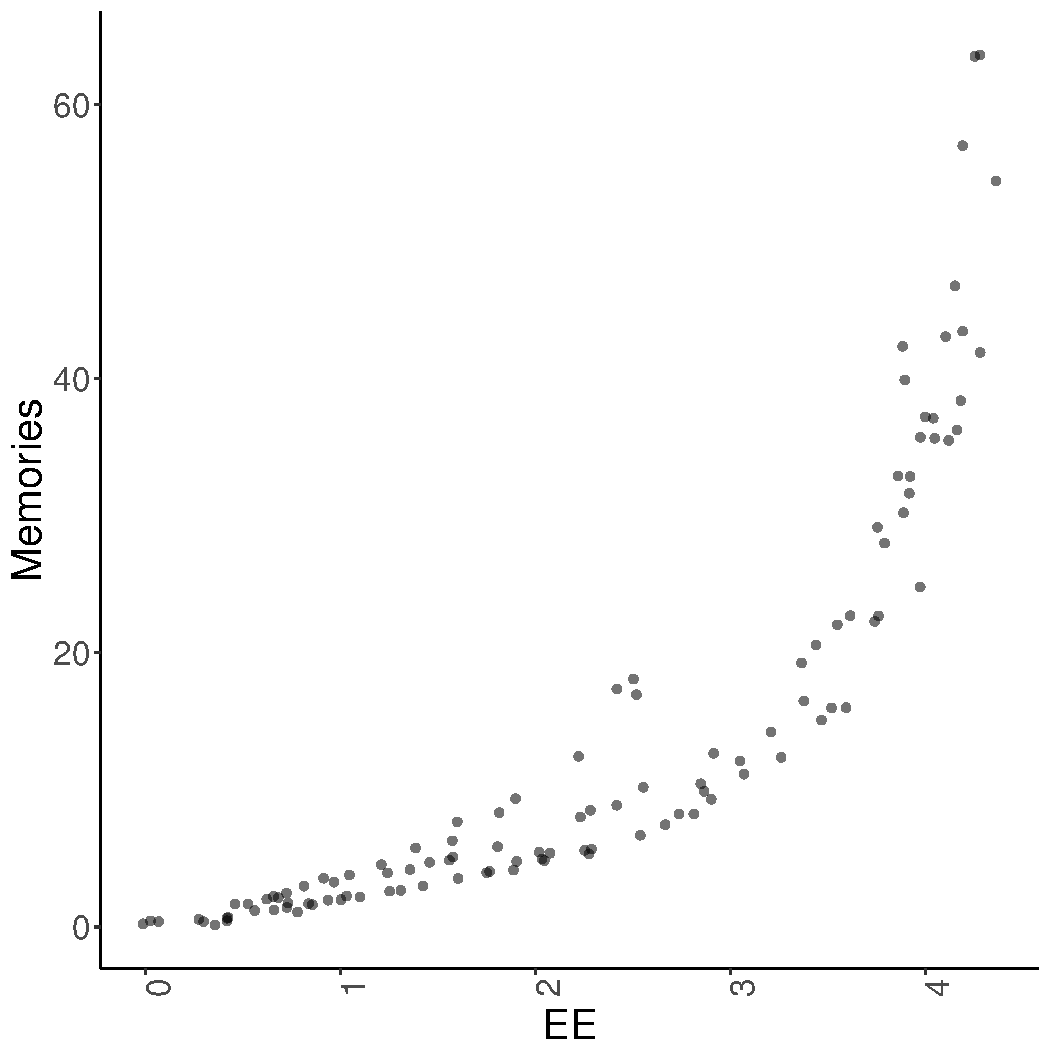
\includegraphics[width=0.3\textwidth]{code/figures/LDC95T8-words-ee-mem.pdf}
%%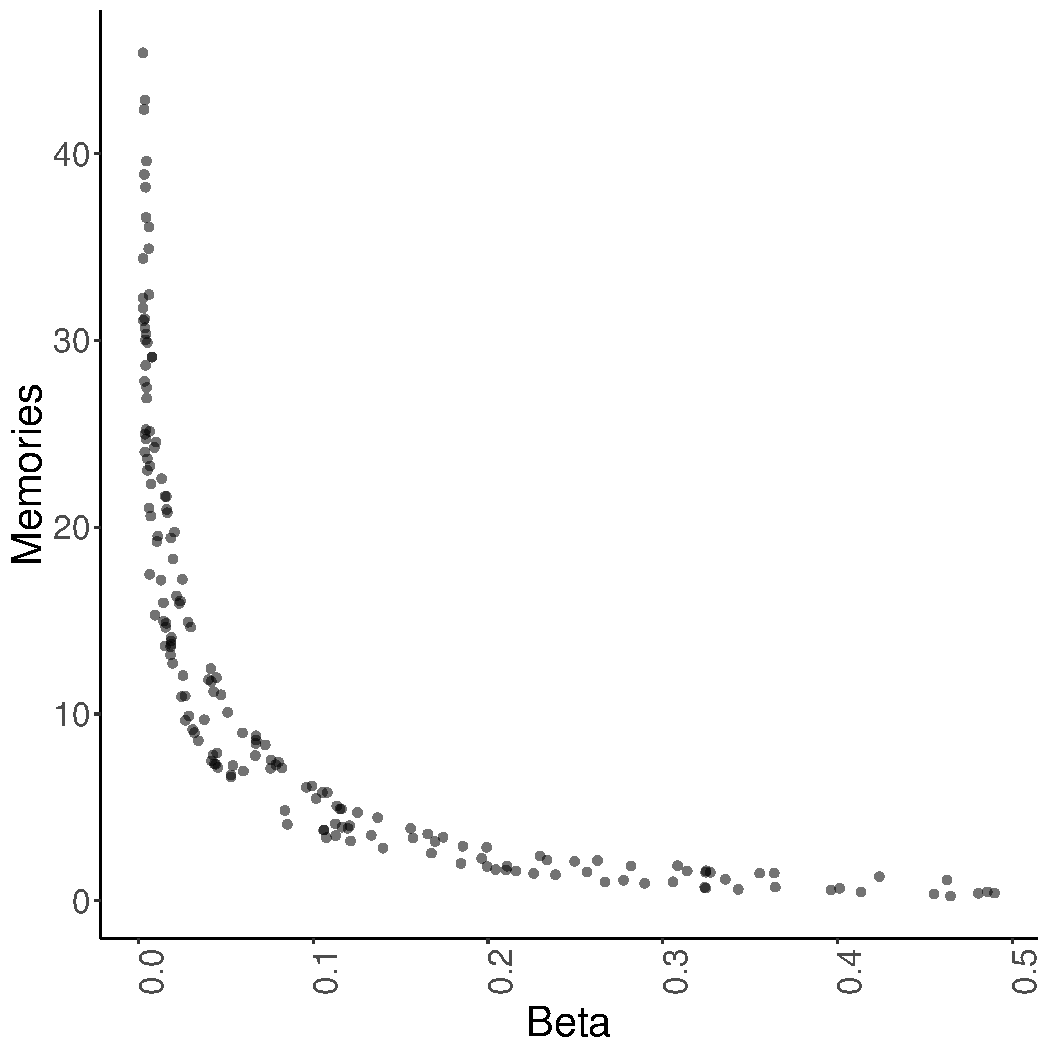
\includegraphics[width=0.3\textwidth]{code/figures/ru-words-beta-mem.pdf}
%\includegraphics[width=0.3\textwidth]{code/figures/LDC95T8-words-nlogbeta-mem-fitted.pdf}
%%\includegraphics[width=0.3\textwidth]{code/figures/LDC95T8-words-logbeta-ee.pdf}
%	\caption{Word-level modeling of Japanese.}\label{fig:jap-logbeta-fit}
%\end{figure*}
%


\begin{figure*}
	\begin{center}
	English

\includegraphics[width=0.3\textwidth]{code/figures/en-words-info-fitted.pdf}
\includegraphics[width=0.3\textwidth]{code/figures/en-words-nlogbeta-mem-fitted.pdf}
\includegraphics[width=0.3\textwidth]{code/figures/en-words-nlogbeta-ee-fitted.pdf}

Russian

	\includegraphics[width=0.3\textwidth]{code/figures/ru-words-info-fitted.pdf}
\includegraphics[width=0.3\textwidth]{code/figures/ru-words-nlogbeta-mem-fitted.pdf}
\includegraphics[width=0.3\textwidth]{code/figures/ru-words-nlogbeta-ee-fitted.pdf}

		Arabic

		\includegraphics[width=0.3\textwidth]{code/figures/ar-words-info-fitted.pdf}
\includegraphics[width=0.3\textwidth]{code/figures/ar-words-nlogbeta-mem-fitted.pdf}
\includegraphics[width=0.3\textwidth]{code/figures/ar-words-nlogbeta-ee-fitted.pdf}
	\end{center}
	\caption{Word-level results.}\label{fig:ar-logbeta-fit}
\end{figure*}



\begin{figure*}
	\begin{center}
	Japanese

\includegraphics[width=0.3\textwidth]{code/figures/LDC95T8-words-info-fitted.pdf}
\includegraphics[width=0.3\textwidth]{code/figures/LDC95T8-words-nlogbeta-mem-fitted.pdf}
\includegraphics[width=0.3\textwidth]{code/figures/LDC95T8-words-nlogbeta-ee-fitted.pdf}

		Chinese

		\includegraphics[width=0.3\textwidth]{code/figures/LDC2012T05-words-info-fitted.pdf}
\includegraphics[width=0.3\textwidth]{code/figures/LDC2012T05-words-nlogbeta-mem-fitted.pdf}
\includegraphics[width=0.3\textwidth]{code/figures/LDC2012T05-words-nlogbeta-ee-fitted.pdf}
	\end{center}
	\caption{Word-level results (cont.).}\label{fig:LDC2012T05-logbeta-fit}
\end{figure*}






\section{Conclusion}
We introduce Neural Predictive Rate Distortion (NPRD), a method for estimating predictive rate-distortion when only sample trajectories are given.
Unlike OCE, the most general prior method, NPRD scales to long sequences and large state spaces.
On analytically tractable processes, we show that it closely fits the analytical rate-distortion curve and recovers the causal states of the process.
On POS-level modeling of natural language, it agrees with OCE in the setting of low rate and short sequences; outside these settings, OCE fails due to combinatorial explosion and overfitting, while NPRD continues to provide estimates.
Finally, we use NPRD to provide the first estimates of predictive rate-distortion for modeling natural language.


\bibliographystyle{apalike}
%\bibliography{extracted}
\bibliography{literature}



\end{document}






















\section{Theoretical Discussion}


\subsection{A Family of Examples}
We present a family of processes that have finite excess entropy and infinite statistical complexity, and which may provide a simple mathematical model of some aspects of language structure.


\begin{defin}
Let $\mu$ be any distribution on the nonnegative integers such that $\mu(0) > 0$.
Then consider the process $(X_t)_t$ where the marginal of $X_t$ is uniform on $\{0,1\}$, and where $X_t$ is generated by (i) taking an independent sample $k \sim \mu$, and (ii) setting $X_t := X_{t-k}$ if $k > 0$, and $X_t$ a fresh uniform draw from $\{0,1\}$ if $k=0$.
\end{defin}

\begin{remark}
I don't know to what extent it is `obvious' that such a process actually exists. I think one can show it by taking the product of the process $K_i \sim_{iid} \mu$, which leads to a partitioning of $\mathbb{Z}$ into equivalence classes of positions that must have the same value in $(X_i)_i$, together with an iid p=1/2 Bernoulli process, which supplies the values to these equivalence classes. Formally, $(X_i)_i$ is then a measurable function of a product of the $K_i$ process and a Bernoulli process, and thus exists.
By marginalizing out $K_i$ given $X_t$, one can verify that this process has the property used to define it in the definition.
\end{remark}

%and the iid p=1/2 Bernoulli process, and condition on $X_$

%\textbf{TODO} is it clear that this process actually exists? Can we invoke Kolmogorov extension thm? Or is this trivial? In any case, we can approximate it by n-th order Markov processes whose excess entropies stay bounded whereas their statistical complexities go to infinity (and which converge to the intended process in average KL distance) (?) In this sense, it may not be a disaster if the process turned out not to exist (?)


Let us first consider how such a process may relate to natural language.

TODO talk a bit about dependencies, agreement, ...



We can prove that it has finite excess entropy and infinite complexity under very general conditions:

%Now examine its statistical complexity and excess entropy:

\begin{proposition}
The following two statements hold:

If $\mu$ has infinite support (i.e., $\#\{k : \mu(\{k\}) > 0\} = \infty$), then $(X_t)_t$ has infinite statistical complexity.

If $\E_{k\sim \mu}[k^2] < \infty$, then $(X_t)_t$ has finite excess entropy.
\end{proposition}
There are many measures $\mu$ that satisfy both constraints, e.g. $\mu(x) \propto 2^{-x}$ or $\mu(x) \propto x^{-4}$.

\begin{proof}
We first show that the process has finite excess entropy:
\begin{align*}
I[X_{<0}, X_{>0}] &= \sum_{t=1}^\infty t I[X_t, X_0|X_1\dots X_{t-1}] \\
& \leq \sum_{t=1}^\infty t \operatorname{\mu}(\{k : k \geq t\}) \\
&= \sum_{t=1}^\infty \frac{t(t-1)}{2} \operatorname{\mu}(\{t\}) \\
&= \frac{1}{2} \E_{k \sim \mu} \left[k^2-k\right]
\end{align*}
which is finite by assumption.

We now show that the process has infinite statistical complexity.

%In the special case where $\mu(n) = 2^{-n}$, it is clear that the causal states are the semi-infinite pasts.
%In general, I don't know whether that's true, but we can still prove infinite complexity.

%and no loss-less compression of pasts is possible. To see this, consider the probabilities $$P\left(X_T=1|X_1=0,...,X_{T-1}=0; x_{<0}\right) = 1/2 \mu(0) + \sum_{t=T}^\infty 1_{x_{T-t} = 1} \mu(t)$$TODO and then?

Since $\mu$ has infinite support and integrates to a finite value, we can find an infinite ascending sequence $0 < t_1 < t_2 < ...$ of integers such that
$$\mu\left(t_i < K \leq t_{i+1}\right) > \mu(K > t_{i+1})$$
for all integers $i$.
Now consider the set $\mathcal{X} \subset \{0,1\}^{\mathbb{N}}$ of semi-infinite sequences that are constant (either 0 or 1) on each interval $t_i, ..., t_{(i+1)}-1$.

We will show that the elements of $\mathcal{X}$ represent distinct causal states.
%Recall that the statistical complexity is defined as the entropy of the causal states.
%(Note that, as $\mathcal{X}$ is uncountable and each of its elements has measure zero, some care has to be taken here.)
%We will show that all the prefixes $x_{1\dots t_i}$ ($i \in \mathbb{N}$), for $x_{1,2,...} \in \mathcal{X}$, 
%$$P\left(X_{t_j}=1|x_{1...t_j-1}; x_{<0}\right) = 1/2 \mu(0) + \sum_{t=t_j}^{t_{j+1}-1} 1_{x_{t} = 1} \mu(t)$$
That is, we show that one can uniquely identify elements of $\mathcal{X}$ from the induced distributions over futures.
Take a semi-infinite sequence $x_{1...} \in \mathcal{X}$.
Assume the distribution $P\left(X_{-1}=1|x_{1}...\right)$ is known, and $x_{1}...x_{t_i-1}$ have already been identified from it.
Then 
$$P\left(X_{-1}=1|x_{1}...\right) = 1/2 \mu(0) + \sum_{t=1}^{t_{i}-1} 1_{x_{t} = 1} \mu(t) + \sum_{t=t_i}^\infty 1_{x_{t} = 1} \mu(t)$$
where $1/2 \mu(0) + \sum_{t=1}^{t_{i}-1} 1_{x_{t} = 1} \mu(t)$ is already a known quantity.
For the remaining part $C_i := \sum_{t=t_i}^\infty 1_{x_{t} = 1} \mu(t)$, we have
$$C = \sum_{t=t_i}^\infty 1_{x_{t} = 1} \mu(t) = \sum_{t=t_i}^{t_{i+1}-1} 1_{x_{t} = 1} \mu(t) + \sum_{t=t_{i+1}}^\infty 1_{x_{t} = 1} \mu(t)$$
which is equal to 
$$\mu(\{t_i...t{i+1}-1\}) + \sum_{t=t_{i+1}}^\infty 1_{x_{t} = 1} \mu(t)$$
or
$$\sum_{t=t_{i+1}}^\infty 1_{x_{t} = 1} \mu(t)$$
depending on whether $X$ is $1$ or $0$ on the set $\{t_i...t_{i+1}-1\}$. Given that 
$$\sum_{t=t_{i+1}}^\infty 1_{x_{t} = 1} \mu(t) \leq \mu(K \geq t_{i+1}) < \mu(\{t_i...t{i+1}-1\})$$
by assumption, the block $x_{t_i...t{i+1}-1}$ can be identified from $C_i$.
%TODO rewrite this
%- first identify the first block
%- then shift, can compute remainder
%Now for any $t_j$ consider the probability
%$$P\left(X_{t_j}=1|X_1=0,...,X_{t_j-1}=0; x_{-1}...x_{t_i-t_j}\right) = 1/2 \mu(0) + \sum_{t=t_j}^{t_{j+1}-1} 1_{x_{t} = 1} \mu(t) + \sum_{t=t_{j+1}}^{\infty} 1_{x_{t} = 1} \mu(t)$$
%where $x_{<0} \in \mathcal{X}$.
%By the previous inequality, this probability is sufficient to identify whether $X_{t_{j-1}}...X_{t_j-1}$ is identically 0 or 1.
Thus, the elements of $\mathcal{X}$ yield different distributions over future observations, and thus represent distinct causal states of the process (modulo the complication that each of them has measure zero).

Indeed, we have shown that the prefixes $x_{1\dots t_i}$ ($i \in \mathbb{N}$), for $x_{1,2,...} \in \mathcal{X}$, represent disjoint sets of causal sets.
For all integers $i$ and any sequence $X_1^\infty \in \mathcal{X}$, the block $x_{1...t_i}$ has log-probability at least $t_i \log \frac{\mu(0)}{2} = \Theta(t_i)$.
Thus
$$H[X_1...X_{t_i} | X \in \mathcal{X}] \geq  t_i \log \frac{\mu(0)}{2} = \Theta(t_i)$$
In conclusion, the statistical complexity is infinite.


%For any positive integer $T$ and any string $x_1...x_T \in \{0,1\}^T$, we have $\log P(X_1...X_T=x_1...x_T) \geq T \log\frac{\mu(\{0\})}{2}$, showing that $$H[X_1...X_T] \geq T \log\frac{\mu(\{0\})}{2} \rightarrow_{T \rightarrow\infty}\infty$$

\end{proof}


\paragraph{Bounding the PRD Curve}
We can bound the predictive rate-distortion curve of this process as follows:
Using an $n$-word context incurs rate at least $n \log \frac{\mu(0)}{2}$, and distortion at most $\sum_{k > n} (k-n) \mu(k > n)$. That is, the faster $\mu(t)$ goes to zero as $t \rightarrow \infty$, the more favorable the prediction-rate tradeoff is (as far as quantified by this upper bound).
%Matching with our results for natural language would suggest $\mu(k>n) \sim n^{1/\beta-1} \exp(-\Theta(n^{1/\beta}))$ -- that is, we expect the probability of long dependencies (within sentences) to decay very fast.


We consider a code $Z_T$ that stores the last $T$ bits.
The rate of this code is $\Theta(T)$ (since $\mu(0) > 0$).
(This code might not be optimal.)


Its distortion is $I[X_{\leq 0}, X_{>T}|X_{1\dots T}]$.
This is upper-bounded by the probability that any future $K$ would reach back to a bit earlier than the last $T$ bits.\footnote{
\begin{align*}
I[X_{\leq 0}, X_{>T}|X_{1\dots T}] & = \sum_{t=T}^\infty (t-T) I[X_t, X_0|X_1\dots X_{t-1}] \\
& \leq \sum_{t=T}^\infty (t-T) \operatorname{\mu}(\{k : k \geq t\}) \\
& = \sum_{t=1}^\infty t \operatorname{\mu}(\{k : k \geq t+T\}) \\
&= \sum_{t=1}^\infty \frac{t(t-1)}{2} \operatorname{\mu}(\{t+T\}) \\
&= \sum_{t=T}^\infty \frac{(t-T)(t-1-T)}{2} \operatorname{\mu}(\{t\}) \\
&= 1/2 \cdot \E[(k-T)_+^2-(k-T)_+]
\end{align*}}
and a lower bound can similarly be derived. \footnote{$I[X_t, X_0|X_1\dots X_{t-1}]$ is at least the probability that the block did not copy from $X_0$, but $X_t$ does.
This is $(1-\mu(1))\dots(1-\mu(t-1))\mu(t)$. So we get
\begin{align*}
I[X_{\leq 0}, X_{>T}|X_{1\dots T}] & = \sum_{t=T}^\infty (t-T) I[X_t, X_0|X_1\dots X_{t-1}] \\
& \geq \sum_{t=T}^\infty (t-T) (1-\mu(1))\dots(1-\mu(t-1))\mu(t) \\
& \geq \left(\sum_{t=T}^\infty (t-T)\mu(t) \right) \left( \prod_{j=1}^\infty (1-\mu(j))\right) \\
& = \E \left[(t-T)_+ \right] \left( \prod_{j=1}^\infty (1-\mu(j))\right) \\
\end{align*}}
We get that the distortion of the code $Z_T$ is bounded as 
\begin{equation}
\E \left[(t-T)_+ \right] \left( \prod_{j=1}^\infty (1-\mu(j))\right) \leq I[X_{\leq 0}, X_{>T}|X_{1\dots T}] \leq 1/2 \cdot \E[(k-T)_+^2-(k-T)_+]
\end{equation}

If $\mu(k) = q^{k} \cdot (1-q)$ (which is a probability distribution over $\mathbb{N}$ for $q < 1$), we have(TODO probably there are algebra errors here)\footnote{$\E \left[(t-T)_+ \right] = \E[k] \mu(k\geq T)$
$\E \left[(t-T)_+^2 \right] = \E[k^2] \mu(k\geq T) = \frac{q+q^2}{(1-q)^2} T q^T (1-q)$, 
$\mu(k\geq T) = T q^T (1-q)$
. where $\phi(q)$ is the Euler function, equal to the Pochhammer symbol $(q;q)_\infty$.}
\begin{equation}
T \frac{q^{T+1}}{1-q}  \phi(q) (1-q) \leq I[X_{\leq 0}, X_{>T}|X_{1\dots T}] \leq 1/2 \cdot (\frac{q+q^2}{(1-q)^2} T q^T (1-q) - T \frac{q^{T+1}}{1-q} )
\end{equation}
and thus
\begin{equation}
I[X_{\leq 0}, X_{>T}|X_{1\dots T}] = \Theta(T q^T)
\end{equation}
In conclusion, we find that $R = \Theta(T)$, $P = \Theta(C-T q^T)$.

Now look at $\mu(k) \sim k^{-t}$ where $t > 3$.
We will take $t$ as a constant here, considering only $T$ as varying.
The infinite product is a (nonzero) constant $C(t)$.
\begin{equation}
\Theta(T^{-t+2} + T^{-t+1}) \leq I[X_{\leq 0}, X_{>T}|X_{1\dots T}] \leq \Theta(T^{-t+3} + T^{-t+2})
\end{equation}
and thus
\begin{equation}
I[X_{\leq 0}, X_{>T}|X_{1\dots T}] = \Theta(T^{-t+2})
\end{equation}
We find that $D = \Theta(R^{-t+1})$, and $\frac{\partial P}{\partial R} = \Theta( R^{-t})$.

%$\frac{\partial P}{\partial R} = \Theta(q^T + T q^T)$


These bounds illustrate some of the kinds of curves that we would expect; however, I don't know how to exactly calculate the curve (as the code $Z_T$ may not be optimal).


\paragraph{Considering Individual Sentences}
This process differs from the setting of individual sentence in that the latter setting involves `boundaries' at which future and past are independent.
We can also construct a variant with this property by taking a distribution $\mu'$ over lengths $1,2,...$, and `resetting' the process in intervals of size $\sim \mu'$, and restricting future copy operations to positions to the right of the last reset point.
This process has statistical complexity %$\Theta(\E_{L \sim \mu'}[L])$: It is clearly upper-bounded by $\E_{L \sim \mu'}[L]$, but also in 
$\Omega\left(\log \frac{\mu(0)}{2} \cdot \E_{L \sim \mu'}[L]\right)$ by the same argument as we developed in the proof of the proposition.
If $\E_{L \sim \mu'}[L] \gg \E_{K \sim \mu}[K^2]$, we obtain a process with finite complexity much larger than its excess entropy, which for all practical purposes may look like its infinite-complexity counterpart.



\paragraph{Prior Work}
Debowski has discussed both the Bernoulli Mixture and the Santa Fe processes as in certain ways  analogous to natural language.
These processes, however, have zero crypticity, so their PRD curves are straight diagonals. (Restricting them to individual sentences would change this.)


%Santa Fe process where each sentence has their own fact collection:
%- best codes just store the facts most likely to be retrieved, to the extent that they are known
%at fixed sentence length
%- predictiveness is larger for concentrated $\mu$
%- smaller for diffuse $\mu$




\subsection{Predictive Rate-Distortion for Processes with Infinite Complexity}
Here we want to show that, even for processes with infinite statistical complexity, the PRD curve provides meaningful quantification of the difficulty of prediction.

\begin{proposition}
Let $(X_t)_t$ be a process such that the entropy $H[X_t]$ is finite (e.g., if the state space is finite).

Then the PRD curve, as a function of Predictiveness, is finite on the interval from 0 to (possibly excluding) the excess entropy.
\end{proposition}

\begin{proof}
An upper bound on the curve is given by the (convex hull) of the pairs of $$\{(H[X_1...X_t], I[(X_1...X_t), X_{>t}]) : t \in \mathbb{N}\}$$
all which are finite under the assumption. 
Also, $$EE = \sup_{t \in \mathbb{N}} I[(X_1...X_t), X_{>t}]$$
So for all values of predictiveness that are strictly below the EE, the corresponding rate has a finite bound.
\end{proof}


\subsection{Sensitivity/Stability of PRD curve}
Unlike statistical complexity, the PRD curve will not differ much between processes that have similar distributions, at least for finite-order Markov processes:


%\begin{proposition}
%	Fix $\epsilon > 0$. % and $M \in \mathbb{N}$.
%	Let $(Y_t)_t$ be a process distributed according to $Q$, and assume that it is close to $X_t$ (distributed according to $P$) in KL Divergence in the following sense: For all $M \in \mathbb{N}$,
%	$$\E_{X_{-\infty}...X_0} \left[\log \frac{P(X_1\dots X_{M}|X_{-\infty}...X_0)}{Q(X_1\dots X_{M}|X_{-\infty}...X_0)}\right] < \epsilon$$
%%	$$\E_{X_{-\infty}...X_0} \left[\log \frac{P(X_1|X_{-\infty}...X_0)}{Q(X_1|X_{-\infty}...X_0)}\right] < \epsilon$$
	%$D_{KL}((X_{1...M}) || Y_{1...M} | \overleftarrow{X}) < \epsilon H[S_0]$.
%	Then the predictive rate-distortion curve of $(Y_t)_t$ is, up to $\epsilon$, a (pessimistic) upper bound on the curve of $(X_t)_t$.
%\end{proposition}


%$$\sup_{f : \|f\|_\infty = 1}  \sum_(f(\overrightarrow{X}, X_1))   $$


The total variation distance between two probability measures $P, Q$ on a discrete space is defined as
		$$D_{TV}(P,Q) := \sum_{x} \left|P(x) - Q(x)\right|$$
	

As a corollary, we can conclude that the PRD curve is a continuous function of the process $(X_t)_t$, in the following sense.
We view the PRD curve as a function defined on all of $\mathbb{R}_+$ by viewing it as a function of the rate.
Then we have:

%, as a set in $\mathbb{R}^2$. %The Hausdorff distance between two curves $c_1, c_2$ is ... %let's say a sequence of curves $c_n$ converges uniformly to a curve $c$ if 
%$$\lim_{n\rightarrow\infty} \sup_{x \in c_n} \inf_{y \in c} \|x-y\| = 0$$


%We say that a process $P_n$ weakly converges to a process $P$ if for all bounded functions $f$



\begin{corollary}
Assume $P, P_n$ are the distributions of $M$-th order Markov processes ($M$ fixed). If $P_n \rightarrow P$ in the following sense
%$$D_{KL}(P_n(\cdot|X_{<0}) || P(\cdot|X_{<0})) \rightarrow 0$$
%$$D_{KL}(P(\cdot|X_{<0}) || P_n(\cdot|X_{<0})) \rightarrow 0$$
%$$D_{TV}(P, P_n) \rightarrow 0$$
		$$D_{TV}(P_n(X_{1\dots M}), P(X_{1\dots M})) \rightarrow 0$$
and if $P_n(x_{1\dots M}) = 0$ whenever $P(x_{1\dots M}) = 0$,
then the PRD curve of $P_n$ converges to the PRD curve of $P$ uniformly on all of $\mathbb{R}_+$.

%TODO verify this!
\end{corollary}




\begin{lemma}
Fix $\epsilon$ and $M \in \mathbb{N}$.
Let $(X_t)_t \sim P$, $(Y_t)_t \sim Q$ be two $M$-th order Markov processes. Assume that the two distributions are close in the following sense:
Further, choose $0 < K < +\infty$ such that
	$$- \log P_Y(X_1=x|X_{-\infty}...X_0) \leq K < +\infty$$
	for all $x$ such that $P_X(X_1=x|X_{-\infty}...X_0) > 0$.
For each point $(R,P$) on the PRD of $(Y_t)_t$, the point $(R+\epsilon \cdot \log |S| \cdot M \cdot \exp(K), P - \epsilon \cdot \log |S| \cdot M \cdot \exp(K))$ is an upper bound on the PRD of $(X_t)_t$.
\end{lemma}




\begin{proof}
Let $Z(x_{<0})$ be a code achieving $(P,R)$ on the PRD of $(Y_t)_t$.
When applied to pasts sampled from $(X_t)_t$, it results in rate
\begin{align*}
\sum_{x_{-M...-1}} P_X(x_{-M...-1}) \sum_z p(z|x_{-M...-1}) \log \frac{p(z|x_{-M...-1})}{p_X(z)} \leq \sum_{x_{-M...-1}} P_X(x_{-M...-1}) \sum_z p(z|x_{-M...-1}) \log \frac{p(z|x_{-M...-1})}{p_Y(z)}
\end{align*}
We always know that $- \left(\sum_z p(z|x_{-M...-1}) \log \frac{p(z|x_{-M...-1})}{p_Y(z)}\right) \leq \frac{I[Z,X]}{\exp(-K)} \leq \log |S| \cdot M \cdot \exp(K)$.
Therefore
\begin{align*}
\left|\sum_{x_{-M...-1}} (P_X(x_{-M...-1}) - P_Y(x_{-M...-1})) \sum_z p(z|x_{-M...-1}) \log \frac{p(z|x_{-M...-1})}{p_Y(z)}\right| \leq \epsilon \cdot \log |S| \cdot M \cdot \exp(K)
\end{align*}


A similar argument holds for predictiveness.



%Also, the predictiveness is
%$$D_{KL}(P_Y(

%$$\leq \E_X \log Q_Y(Z) - \E_Y \log Q_Y(Z) $$

%Storing $S'_0$ and predicting the future on its basis results in $\epsilon H[S_0]$ additional loss in the future.
\end{proof}


\begin{proof}




\end{proof}





More generally, if $Z$ for a bounded rate amounts to a Markov approximation for bounded length $M$, will still get locally uniform convergence.

Convergence of Markov approximations:

-- code can be computed from context M with high probability

-- 


%	Then the predictive rate-distortion curve of $(Y_t)_t$ is, up to $...\epsilon$, a (pessimistic) upper bound on the curve of $(X_t)_t$:
%	For a given level of rate, the achieved predictivity of $(X_t)_t$ at this rate is at least the predictivity of $(Y_t)_t$ at this rate minus $...\epsilon$.
	


Such a continuity statement is not true for statistical complexity (see the next example).

\begin{example}[Simple Example]
Here is a very simple example with $M=1$.
Let $S$ be a finite set.

Process 1, with distribution $P$, consists of IID uniform draws from $S$. . %\log |S|$. % ($\{0,1\}^\mathbb{Z}$).

Process 2, with distribution $P_n$, chooses $X_{t+1}$ to be $X_t$ with probability $1/n$, and a new independent uniform draw from $S$ otherwise. 

The statistical complexity is $0$ for $P$, but $\log |S|$ for any $P_n$, independent on $n$. In contrast, the PRD curve of $P_n$ converges to the PRD curve of $P$, which is the set $\mathbb{R}_+ \times \{0\}$: For any given rate, one can only achieve zero predictiveness for a process of IID samples.
The PRD curve of $P$ converges to that curve, as maximum achievable predictiveness goes to zero as $n\rightarrow \infty$.
\end{example}

I don't know how to prove anything like this when the processes do not have uniformly bounded Markov order.

In Lohr CITE it was shown that statistical complexity is lower weak-$^*$ semicontinuous, for general stochastic processes.
I don't know whether the same holds for the PRD curve.


Limitation in the case of unbounded Markov order: Process that copies symbol from $M$ words in past. Does this converge to iid Bernoulli weakly, since the finite products of single-variable indicators converge?
\url{https://mathoverflow.net/questions/106234/simple-functions-on-a-product-measure-space}
The PRD curves don't converge.


%\begin{proposition}
%	Fix $\epsilon_1, \epsilon_2 > 0$ and $M \in \mathbb{N}$.
%	Let $(Y_t)_t$ be a process distributed according to $Q$, and assume that it is close to $X_t$ (distributed according to $P$) in KL Divergence in the following sense:
%	$$\E_{X_{-\infty}...X_0} \left[\log \frac{P(X_1\dots X_{M}|X_{-\infty}...X_0)}{Q(X_1\dots X_{M}|X_{-\infty}...X_0)}\right] < \epsilon_1$$
%	Further, assume $I[X_{>M}, X_{<0}|X_{1...M}] < \epsilon_2$.
%	$$\E_{X_{-\infty}...X_0} \left[\log \frac{P(X_1|X_{-\infty}...X_0)}{Q(X_1|X_{-\infty}...X_0)}\right] < \epsilon$$
	%$D_{KL}((X_{1...M}) || Y_{1...M} | \overleftarrow{X}) < \epsilon H[S_0]$.
%	Then the predictive rate-distortion curve of $(Y_t)_t$ is, up to $\epsilon_1 + \epsilon_2$, a (pessimistic) upper bound on the curve of $(X_t)_t$:
%	For a given level of rate, the achieved predictivity of $(X_t)_t$ at this rate is at least the predictivity of $(Y_t)_t$ at this rate minus $\epsilon_1+\epsilon_2$.
	
%	TODO but the rate will also change???
%\end{proposition}

















\paragraph{Difficulty of Estimating Statistical Complexity}
We now contrast this with estimating full statistical complexity, which is much harder.

Informally, the difficulty with estimating statistical complexity is that processes that differ only minimally in their distribution over trajectories can have widely different complexities.

%
%For finite-state processes, complexity can be estimated in the limit of infinite data, by constructing Hidden Markov Models that incorporate successively more complexity.
%
%However, estimation from a fixed finite dataset is limited.

One may expect that this will hinder estimation of statistical complexity from data.
Here, we formalize this in a statistical estimation setting by considering the problem of providing bounds on complexity from data, specifically constructing confidence intervals.

Lower bounds on statistical complexity can be constructed from finite data by estimating the excess entropy.
When the Markov order $k$ is finite and known, the logarithm of the number of possible sequences of length $k$ clearly upper-bounds statistical complexity.
It is not hard to show that finite data does not allow one to construct a better upper bound:
Any confidence interval for statistical complexity that has good coverage (e.g., $95 \%$) needs to include this trivial upper bound most of the time (e.g., more than $95 \%$).


\begin{proposition}
Fix a positive integer $k$ and a space $S$ of observable states.
Let $\mathcal{X}$ be the class of stochastic processes that are of Markov order $\leq k$, taking values in $S$.
%Let $(X_t)_t$ be any process.
% taking values in $S$.
%Fix any $N$ be the number
Then no confidence interval for the statistical complexity of processes from $\mathcal{X}$, with coverage $\beta > 0$ (e.g., 0.95), can exclude the `trivial' upper bound $k\log S$ with probability $\gamma > 1-\beta$ (e.g., $> 0.1$)%for any generating process
, no matter how many datapoints have been collected.
\end{proposition}

\begin{proof}
For a contradiction let a confidence interval be given, and assume it excludes $k\log |S|$ with probability $\gamma > 1-\beta$ for some process, for $n$ datapoints.
We can consider a process which only differs a tiny bit but has statistical complexity $k\log |S|$, and for which the probability distribution over $n$-datapoint datasets will differ by at most $\epsilon$, chosen such that $1-\beta + \epsilon < \gamma$.
Then, applied to this process, the CI will exclude $k \log S$ with probability $\geq \gamma-\epsilon$, so has coverage $\leq 1-\gamma+\epsilon < \beta$, contradiction.
\end{proof}

One can easily extend this to see that, if all available sample trajectories have length $\leq k$, a confidence interval can never exclude $k \log |S|$ for any nonzero coverage, irrespective of the number of datapoints available.


Contrast this with PRD:
By running a method such as OCE or NPRD on held-out data, one can obtain a high-probability bound on the PRD curve.
TODO that's not actually totally clear to me




%
%This condition is sufficient but not necessary.
%%For instance, for the states $S_0$ of the full $\epsilon$ machine, one could substitute the states of 
%
%
%$K_M := H[S_0|X_{-M\dots 0}]$ is an upper bound on the statistical complexity
%
%$K_M := I[S_0, X_{-M\dots 0}]$ is a lower bound on the statistical complexity
%
%the statistical complexity of the $2M$-order Markov approximation is a lower bound on the statistical complexity
%
%If $I[S_0, X_{\leq 0}] - K_M \epsilon$, then predictive rate-distortion estimated with trajectories of length $M$ will be close to tight.
%
%In general, if $X_{-T...0}$ leads to low distortion, this does not mean that 
%
%(can always also get a lower bound)
%
%%The rate-distortion tradeoff curve is uniformly $\epsilon$-close at length $T$ if and only if the statistical complexity of the $T$-order Markov approximation is $\epsilon$-close to the full statistical complexity for predicting the next $M$ words.
%%$$\inf_{Z \rightarrow X_{-M...0} \rightarrow X_{1...M} : I[Z, X_{1...M}] = H[Z]} H[Z]$$
%%$$\inf_{Z \rightarrow X_{-\infty...0} \rightarrow X_{1...M} : I[Z, X_{1...M}] = H[Z]} H[Z]$$
%
%or 
%$K_M := I[S_0, X_{-M\dots 0}]$
%
%
%
%
%
%Convexity of tradeoff function
%


%\section{Discussion}
%
%In (\ref{eq:bound}), we upper-bounded $I[Z, (X_{-T\dots -1})]$ using $D_{KL}(N(\mu, \sigma^2) || q)$.
%There are other ways of approximating $I[Z, (X_{-T\dots -1})]$ that (for fixed $Z$) give a lower bound instead of an upper bound.
%As a result, the solutions will not be guaranteed to be an upper or lower bound on the theoretical solutions of the actual problem (\ref{eq:ib}), but the approximation may be tighter.
%
%-adversarial (by reconstructing past)
%
%- adversarial (deciding whether or not belong together)
%
%-dual




\section{Theoretical Guarantees}


%\begin{proposition}
%Estimating predictive rate-distortion, excess entropy
%
%- known Markov order $k$
%
%- constructing $95 \%$ CIs?
%
%can both upper-bound and lower-bound
%
%We can construct CIs by combining CIs for upper bounds and for lower bounds.
%For the upper bounds, can take any relevant algorithm on fresh data.
%For lower bound, create CI for mutual informations; can use this to lower bound
%
%
%\end{proposition}
%
%

%think about a process with finite excess entropy, such that pasts of length $T$ incur KL distortion $\epsilon$

Our method provides a bound on the PRD curve.

How close can we expect the bound be to the actual curve?
For a given process, this will depend on the number $N$ and the length $T$ of the available sample trajectories.
As long as $T$ is smaller than the Markov order of the process -- so in particular for infinite Markov order processes, the bound need not be tight even for infinite sample size $N$.
Intuitively, two conditions need to be satisfied to guarantee a good bound:
It must be possible to infer sufficient information about the state of the epsilon machine from pasts of bounded length, and most of the predictive power of the state must be `used' in the near future.
This is formalized by the following result.
We say that an estimated curve is $\epsilon$-\emph{close} to the true curve if, for every point of the true curve, some point on the estimated curve has distance $\leq \epsilon$ in $\ell_1$ distance.



\begin{proposition}
Fix $\epsilon > 0$.
Assume that
	\begin{enumerate}
		\item The probability mass of sequences $X_{-M\dots 1}$ from which $S_0$ can be uniquely identified is at least $1-\epsilon$. More formally,
	$$ P\left(\{X_{-M\dots 1} : \#\{S_0 : P(S_0|X_{-M\dots 1}) > 0\}\}\right) \geq 1-\epsilon  $$
\item	$\frac{I[S_0, X_{M+1...\infty}|X_{1...M}]}{H[S_0]} < \epsilon$
	\end{enumerate}
%Assume that the epsilon machine has $\epsilon/2$-mixing time $< M$ (in the sense that $I[S_0, S_M] < \epsilon/2$), 
	Then the predictive rate-distortion curve of the $2M$-order Markov approximation is $3\epsilon H[S_0]$-close to the curve of $(X_t)_t$.
	%Assume that $H[S_0|X_{-M\dots 1}] < \epsilon/2$ and that
\end{proposition}

\begin{proof}
	Let a point on the curve be given, with a solution $S'_0$ that is a (stochastic) function of $S_0$.
Let $Z$ be $S'_0$ if $S_0$ is identifiable and some uniformly random state otherwise.
	Then
	\begin{equation}
		I[S'_0, \overleftarrow{X}] - \epsilon H[S'_0]\leq	I[Z, X_{-M, ..., 0}] \leq I[S'_0, \overleftarrow{X}]
	\end{equation}
	\begin{equation}
		I[S'_0,\overrightarrow{X}] \geq 	I[Z, X_{1...M}] \geq I[S'_0, X_{1...M}] - \epsilon H[S'_0] \geq I[S'_0, \overrightarrow{X}] - I[S'_0, X_{M+1...\infty}|X_{1...M}] - \epsilon H[S'_0] \geq I[S'_0, \overrightarrow{X}] _ 2\epsilon H[S'_0]
	\end{equation}
\end{proof}

Unlike statistical complexity, the tradeoff will not differ much between processes that have similar distribution:

\begin{proposition}
	Fix $\epsilon > 0$ and $M \in \mathbb{N}$.
	Let $(Y_t)_t$ be a process distributed according to $Q$, and assume that it is close to $X_t$ in KL Divergence in the following sense:
	$$\E_{X_{-\infty}...X_M} \left[\log \frac{P(X_1...X_M|X_{-\infty}...X_0)}{Q(X_1...X_M|X_{-\infty}...X_0)}\right] < \epsilon$$
%	$D_{KL}((X_{1...M}) || Y_{1...M} | \overleftarrow{X}) < \epsilon H[S_0]$.
	Then the predictive rate-distortion curve of $(X_t)_t$ is, up to $\epsilon$, a (pessimistic) bound on the curve of $(Y_t)_t$.

\end{proposition}

\begin{proof}
Storing $S'_0$ and predicting the future on its basis results in $\epsilon H[S_0]$ additional loss in the future.
\end{proof}

In particular, if we can find a process $Y_t$ for which the conditions in the proposition above hold, and which is close to $X_t$ in both directions of the KL Divergence, then we can guarantee good approximation to the predictive rate-distortion curve of $X_t$.

%\begin{proposition}
%	Fix $\epsilon > 0$ and $M \in \mathbb{N}$.
%	Let $(Y_t)_t$ be a process satisfying the conditions of the previous proposition, distributed according to $Q$, and assume that
%	$$\E_{X_{-\infty}...X_M} \left[\log \frac{P(X_1...X_M|X_{-\infty}...X_0)}{Q(X_1...X_M|X_{-\infty}...X_0)}\right] < \epsilon H[S_0]$$
%%	$D_{KL}((X_{1...M}) || Y_{1...M} | \overleftarrow{X}) < \epsilon H[S_0]$.
%	Then the predictive rate-distortion curve of the $2M$-order Markov approximation of $(Y_t)_t$ is $5\epsilon H[S_0]$-close to the curve of $(X_t)_t$.
%
%\end{proposition}
%
%\begin{proof}
%Storing $S'_0$ and predicting the future on its basis results in $\epsilon H[S_0]$ additional loss in the future.
%\end{proof}

%This proposition shows that good estimation of rate-distortion tradeoff can be guaranteed if it can be guaranteed for a `similar' but more well-behaved process $Q$.



%
\begin{abstract}



%\mhahn{TODO the abstract will go here} % write abstract}
%%LSTMs prefer language, and they prefer languages that show stronger locality even more
%
%%Psycholinguistic research has established that human language processing shows locality effects, and has linked this to effects of memory in incremental processing.
%%We first show that common sequence models are biased towards word orders as occur in natursl language, and that this bias is stronger for languages with fixed word order.
%% We then show that optimizing word order for ease of LSTM language modeling makes valid typological predictions about language: It predicts a preference for 
%
%

We describe a general formalization of incremental prediction under memory limitations that makes no assumptions about architecture and the memory representations, beyond incremental modeling with bounded memory.
Using data from 50 diverse languages, we then use our framework to provide evidence that word orders in human language are optimized for memory demands in incremental prediction.
\end{abstract}



Work has argued that natural language orders information in ways that reduce memory effort, and similar claims.

- center embeddings dispreferred

- explanation of greenberg universals

- dependency length minimization

Some work quantifying memory:

- grammars, but then will depend on assumptions about the parsing architecture

Our contributions:

- describe an information-theoretic measure of memory load, which is an assumption-free lower bound on average memory cost in incremental prediction

- the link between memory boundedness and locality falls out of it, without assuming memory decay (strong relation to Noisy-Context surprisal, but without assumption of decay)

- computational study on X languages provides evidence that their word orders help lower memory cost --> large scale evidence

-- simulations on level of POS

-- simulations on level of morphology

-- simulations on level of morphology + lemmas

- simulations show a close link to dependency length minimization, supporting an explanation of DLM in terms of memory bounds in incremental prediction

-- correlation of memory and dependency length

-- using optimized languages

-- ? Masha's data

\section{Formalizing and measuring information locality}

locality proposed in many forms as (1) making human language processing easier, (2) a principle shaping word order in language.
Among (1), prominent examples are Dependency Locality and cue-retrieval theories of sentence processing.
For (2), the principle of Dependency Length Minimization has become prominent, and it had a number of precursors (Behagel 1930, Rijkhoff 1986, Hawkins 1990).
It is widely assumed that (2) is due to (1).

(1) has been viewed as contradictory or complementary to prediction-based theories of processing.
Recently, CITE described a model of prediction under memory limitations that unifies both theories. % information-theoretic formalization based on incremental prediction, show that it predicts information locality

They also showed that it predicts a principle they called information locality.

They further argued that information locality predicts that long dependencies are harder to process, accounting for (1) and (2).

In particular, this makes the prediction that languages are optimized for information locality, but it leaves open the question of  how to rigorously define informatuion locality to test whether languages optimize it.



\subsection{Memory and Locality in General Sequence Models}

We consider a general incremental listener who maintains an internal memory state and, in each time step, and attempts to predict the next symbol (word, phoneme, ...) by computing a distribution over the vocabulary, based on its memory state, and then updates its memory state on the basis of the received word. %, stochastically emits a word from this distribution, and updates its memory state depending on the chosen word.
Time can be discrete or continuous in this model; we'll assume that there are discrete time steps but the math doesn't depend on this.
We are making the technical assumption that the process is stationary, that is, that the rules by which the model manipulates its memory and outputs words do not change over time.
This model describes aspects of human language processing, if we accept that humans perform incremental prediction.

%(Typical NLP models such as n-gram models and LSTM language models also fit into this framework.)
%N-gram models and LSTM language models both fit into this framework.
%On the other hand, LSTM models with random access to prior words do not fit into this framework, as they rely on past states in addition to their internal memory state at time $t$.

In this general model, we can use information theory to relate this listener's surprisal to the size of the memory representation measured in bits.

\emph{No further assumptions about the nature of the memory representations, their implementation, and how they evolve over time enter these results. The only caveat is that it is not clear, a priori, that the information-theoretic bounds on the size of memory representations are relevant for human sentence processing, as understanding memory-related bottlenecks in human processing might necessitate taking the architecture, implementation, etc. of memory into account. Here, we're exploring how much can be shown without reference to any such things. In any case, no matter how memory is implemented in sentence processing, our results provide lower bounds on the size of these representations -- any physical encoding of the past will need to store at least as much information as indicated by our results.}

We first consider the situation where the listener's predictions are optimal, in the sense that no other listener could achieve lower average surprisal (we later explain how our results generalize to the more general case of potentially non-optimal predictions)..

We first look at the average number of bits needed to encode the memory states, which is (essentially) equal to the entropy of the memory state, viewing the memory state as a random variable.
This number decomposes exactly into what I'm inclined to call (1) locality cost, and (2) ambiguity cost.

We let $X_t$ be a process of observations (e.g. words), and $M_t$ be the internal memory states of the listener, which we can take to be a function of $X_{\leq t}$.
Under the assumption of optimality oif predictions and minimality of memory cost, we can take $M_t$ to be an equivalence class of pasts that induce the same distribution over futures (need to be careful for general processes. we here want to add the assumption that, since we are interested in sentence processing, memory is reset entirely at sentence or discourse boundaries, avoiding cases where the math wouldn't work so nicely).

Locality cost:
\begin{equation}\label{eq:locality-cost}
L := \sum_{t=1}^\infty\ t \cdot \operatorname{I}[X_t, X_0 | X_1, ..., X_{t-1}]
\end{equation}

Ambiguity Cost:
\begin{equation}\label{eq:ambiguity-cost}
A := H[M_0|\overrightarrow{X}]
\end{equation}


Note that both terms are nonnegative.



\begin{proof}
By the definitions of conditional entropy and mutual information,
$H[M_0] = H[M_0 | \overrightarrow{X}] + I[M_0, \overrightarrow{X}]$
The first part is Ambiguity cost.
Now we show that the second part is equal to Locality cost.
As we assume that the listeners predictions are optimal, $I[M_0, \overrightarrow{X}] = I[X_{\leq 0}, \overrightarrow{X}]$.
Then the formula is a consequence of the chain rule for mutual information:
\begin{align*}
I[(X_i)_{i > 0}, (X_i)_{i \leq 0}] &= \sum_{i=1}^\infty I(X_i, (X_i)_{i \leq 0}|X_1, ..., X_{i-1}) \\
&= \sum_{i=1}^\infty \sum_{j=0}^{-\infty} I(X_i, X_j|X_{j+1}...X_{i-1}) \\
& = \sum_{t=1}^\infty\ t \cdot \operatorname{I}[X_t, X_0 | X_1, ..., X_{t-1}]
\end{align*}
\end{proof}

Related pointwise quantity:

Relaxing optimality:
The first step in the proof continues to hold

- locality cost: done

- ambiguity cost: find the best partitioning of the past that (1) enables the given surprisal, (2) minimizes the conditional entropy of memory conditioned on future

Relation to prior work:

- Computational Mechanics, long-range dependencies in text, excess entropy

- storage cost in DLT (which is also prediction-based!)

- Hawkins' MiD and MaxOP

- garden paths, and incremental parsing models over the history of PsychoLing: e.g. beam search in Jurafsky 1996 could be linked to Ambiguity Cost

In this general framework, the minimal amount of bits needed to encode the model's internal memory state is related to the decay of mutual information over distances:
The faster mutual information between words decays as their distance increases, the less memory is required.
More precisely:

\begin{proposition}
Modeling a stationary process  $(X_t)_{t \in \mathbb{Z}}$ in this framework %of incremental modeling described above,
 requires maintaining at least
\begin{equation}\label{eq:memory-bound}
M := \sum_{t=1}^\infty\ t \cdot \operatorname{I}[X_t, X_0 | X_1, ..., X_{t-1}]
\end{equation}
bits of memory,
where
$\operatorname{I}[X_t, X_0 | X_1, ..., X_{t-1}]$ is the mutual information of the observations $X_t$ and $X_0$, conditioned on the intervening observations.
\end{proposition}
%that the model does not have an `absolute clock' built into it.
This quantity is also known as the \emph{excess entropy} of the process (CITE).




\begin{proof}
%We assume that the process is stationary, that is, that there is no `absolute clock' built into the model. Formally, this means that, for any set of indices $t_1 < t_2 < \dots < t_n$, the joint distribution $(X_{t_1}, X_{t_2}, ..., X_{t_n})$ only depends on the differences $(t_{i+1}-t_i)_{i=1,...,n-1}$, not on the absolute values $t_i$.
The number of bits of memory is lower bounded by the mutual information between past and future observations, $I[(X_i)_{i>0}, (X_i)_{i \leq 0}]$. 
Then the formula is a consequence of the chain rule for mutual information:
\begin{align*}
I[(X_i)_{i > 0}, (X_i)_{i \leq 0}] &= \sum_{i=1}^\infty I(X_i, (X_i)_{i \leq 0}|X_1, ..., X_{i-1}) \\
&= \sum_{i=1}^\infty \sum_{j=0}^{-\infty} I(X_i, X_j|X_{j+1}...X_{i-1}) \\
& = \sum_{t=1}^\infty\ t \cdot \operatorname{I}[X_t, X_0 | X_1, ..., X_{t-1}]
\end{align*}
%In the last step, we have made the technical assumption that the process is stationary, that is, that the rules by which the model manipulates its memory and outputs words do not change over time.
%that the model does not have an `absolute clock' built into it.
\end{proof}
That is, we measure the amount of statistical dependency of observations that are $t$ steps apart, controlling for any information that is redundant with intervening observations.
This quantifies how much information needs to be carried across $t$ timesteps without any possibility for `guessing' it from intervening observations.

Due to the factor $t$ inside each term of the sum, carrying the same amount of information over longer distances requires more memory -- that is, modeling long statistical dependencies is more costly in terms of memory than modeling shorter ones.
This, in a nutshell, formalizes a general, assumption-free, link between memory and locality in incremental prediction.


The result in (\ref{eq:memory-bound}) is entirely information-theoretic and applies to \emph{any} physical encoding of the past, entirely independent of the implementation of the model and the mechanisms by which it computes predictions.
In particular, while the relation to psycholinguistic and psychological models of how memory works would be interesting to explore, our result applies to any such model.
Memory representations do not have to be rational or optimal for this bound to hold:
It provides a \emph{lower bound} on the amount of information that needs to be stored -- other memory representations will always need to store at least as much information.




\subsection{Tradeoff between Memory Load and Predictability; Information Locality}

%The quantity $\operatorname{I}[X_t, X_0 | X_1, ..., X_{t-1}]$

We want to derive a quantitative measure of Information Locality.

By information locality, we refer to the degree to which words that are predictive of each other are closer together.
Stated differently, information in past observations that helps predict $X_t$ should be concentrated in recent observations $X_{t'}$ ($t' < t$) with $t'$ close to $t$.

Information locality is maximised if all contextual information predicting $X_t$ is contained in $X_{t-1}$, in which case $J = I[X_t, X_{t-1}]$.

To quantify information locality more generally, we consider the relation between the quantity
$$J = I[X_{\geq t}, X_{<t}] = \sum_{t=1}^\infty\ t \cdot \operatorname{I}[X_t, X_0 | X_1, ..., X_{t-1}]$$
and the quantity
$$P = I[X_t, X_{< t}] = \sum_{t=1}^\infty\ \operatorname{I}[X_t, X_0 | X_1, ..., X_{t-1}]$$
The first one quantifies how much information is transmitted between past and future, the second one captures the average predictability of single words from their prior context.
Evidently, $P \leq J$ -- higher degrees of predictability will require more information to be stored from past observations.
Stated differently, there is a tradeoff between predictability and memory: If the future is easier to predict from the past (at the same unconditional entropy), more memory is required to store all the relevant predictive information from the past.

Minimizing $J$ unconditionally corresponds to an entirely unpredictable process.
In contrast, if we minimize $J$ while holding $P$ constant, we obtain a formalization of the requirement of optimal information locality: This requires placing the predictive information closer to the present observation, keeping the total amount of predictive information constant..

If there are no further constraints on the minimization, the minimum is attained when $P = J$.
This is the case when all contextual information predicting $X_t$ is contained in $X_{t-1}$ -- this minimizes memory load, as only information from the last word needs to be stored.
If $P$ is fixed, and $J$ increases, information locality decreases -- corresponding to increasing memory load.

To understand this more generally, let us consider $\operatorname{I}[X_t, X_0 | X_1, ..., X_{t-1}]$ as a function of $t$.
This function describes the amount of bits predictive of $X_t$ contained in $X_0$, the observation $t$ steps in the fast.
The faster this function decays, the lower $J$ is.
Information locality can be interpreted as requiring this function to decay fast -- $J$ is absolutely minimized if the function jumps to zero for $t > 1$.

If this is a principle describing natural language, we expect that there will be further constraints, resulting in values of $J$ larger than $P$.
We will study this in detail in the next section.


We can observe that the area under the curve is equal to $P$ -- this quantifies the total amount of contextual information predicting the current observation.
This suggests to consider the ratio
$$L := \frac{J}{P}$$
First, note that minimizing $J$ with $P$ fixed is equivalent to minimizing $L$.
Second, expanding this quantity, we see
$$L = \sum_{t=1}^\infty t \frac{\operatorname{I}[X_t, X_0 | X_1, ..., X_{t-1}]}{\sum_{t=1}^\infty\ \operatorname{I}[X_t, X_0 | X_1, ..., X_{t-1}]}$$
That is, $L$ describes the $J$-coordinate of the center of mass of the area under the curve in (REF).
A different way of understanding it is as the average distance of past information predictive of the current observation.
With this interpretation of $L$, we can understand it as a direct fornalization of the notion of information locality.

Let  us consider a second visualization by plotting $J$ against $P$.
The area that is achievable by processes is the area below the diagonal.
Information locality is maximized by processes on the diagonal; the distance from the diagonal quantifies the ratio $J/P$ and thus information locality.


%
%Let us consider two methods of visualising $J$ and its relation to $I$.
%First, we can consider $\operatorname{I}[X_t, X_0 | X_1, ..., X_{t-1}]$ as a function of $t$.
%This function describes the amount of bits predictive of $X_t$ contained in $X_0$, the observation $t$ steps in the fast.
%The faster this function decays, the lower $J$ is.
%Information locality can be interpreted as requiring this function to decay fast.
%When we hold this area constant, steeper decays of the curve correspond not only to lower values of $P$, but also to stronger concentration of predictive information in the recent past, and thus to the notion of information locality.
%One way of quantifying the degree of 
%Information locality is maximized when $P = J$.
%This is the case if and only if all contextual information predicting $X_t$ is contained in $X_{t-1}$ -- this minimizes memory load, as only 
%If $P$ is fixed, and $J$ increases, information locality decreases -- corresponding to increasing memory load.
%We can this in Figure (REF): We plot $J$ against $P$.
%The region below the diagional is achievable, with processes on the diagonal minimizing memory load and maximizing information locality.
%The further a process is from the diagonal, the less information locality it has.
%we consider a general model of incremental prediction with boundedness of memory as the only assumption, and derive a notion of information locality.
%Our formulation elegantly generalizes the link between memory limitations and information locality from (CITE) to the setting of arbitrary bounded-memory models


\subsection{Discussion}
\paragraph{Conditional and Unconditional Mutual Information}
Prior work has studied the decay of \emph{unconditional} mutual information $I[X_t, X_0]$ in natural language, and linked it to locality and memory.
However, they decay of unconditional mutual information is less closely linked to memory requirements:
While the decay of conditional mutual informnations provides a lower bound on memory need, unconditional mutual information does not:
Consider the constant process where with probability 1/2 all $X_t = 0$, and with probability 1/2 all $X_t = 1$. %%$X_t = c$, where $c$ is random but independent of $t$ for each specific draw from the process.
The unconditional mutual information is 1 at all distances, so does not decay at all, but the process only requires 1 bit of memory.
Conversely, one can construct processes where the unconditional mutual informations are 0 for all $t$, but where $P > 0$ and this predictive information is actually spread out over arbitrarily large distances (that is, $J/P$ can be arbitrarrily large)..

\paragraph{Hierarchical Structure}
Processing nontrivial hierarchical structures typically requires unbounded amounts of memory.
However, crucially, the \emph{average} memory demand can be finite.
- For PCFGs, a classical probabilistic grammar formalism, one can show that excess entropy is always finite (as is the average memory cost).


\paragraph{Decay vs Interference}
Work has suggested that interference and memory overload is more appropriate than decay (Lewis and Vasisth 2005, p. 408) for modeling locality and memory in sentence processing.
Since excess entropy is a lower bound on any memory representation, it is compatible with any type of memory model.
Nonetheless, the formula in (\ref{eq:memory-bound}) might suggest that boundedness of memory entails that memory has to decay.
This is not the case:
A long dependency can be maintained perfectly with low average memory:
Informally, if every sentence is $N$ words long and has one long-distance dependency spanning the entire sentence, this dependency can be modeled perfectly with a memory cost that is independent of $N$.
In contrast, if every symbol strongly and non-redundantly depends on the character $T$ steps in the past, with $T$ large, this will create a memory cost proportional to $T$.
%In contrast, if every $N$th symbol has such a dependency, the memory cost is only $T/N$.



\paragraph{Relation to DLT Storage Cost}

TODO


\section{Evidence that natural language optimize information locality}

(1) languages optimize information locality, as formalized by (REF)

(2) languages trade off predictability and memory load

-- i. (1) is one way of formalizing this

-- ii. at fixed predictability, languages minimize memory load

-- iii. Pareto property: few hypothetical languages are better in terms of both factors





- information locality and predictability can trade off -- we present large-scale evidence that word orders found in languages optimize this tradeoff / optimize information locality

Do word orders in language minimize memory need as quantified by (\ref{eq:memory-bound}), when compared to other possible orderings?

\subsection{Prediction on the level of POS}
As mutual information cannot be realiably estimated on many of the smaller corpora in the UD project, we first compute (\ref{eq:memory-bound}) on the level of POS tags -- that is, we compute memory need for incremental prediction of POS sequences. %, following~\cite{futrell-noisy-context-2017}.
As the summation in~(\ref{eq:memory-bound}) terminates when $t$ is greater than the length of any sentence, we can compute this quantity exactly for the empirical distribution over sentences in a given corpus.

%We computed these quantitities for the optimized languages, the original languages, and for baseline  languages. For each language, we created 50 baseline ordering models, for which $a_\tau, b_\tau$ where drawn uniformly from $[-1, 1]$.
%As mutual information between words is decreased if the language exhibits additional randomness (as our stochastic ordering models do) -- which decreases memory demands but increases entropy -- we hold the entropy of our languages constant by replacing each sampling step with taking the maximum -- that is, we take the zero temperature limit.
%This ensures that all versions of a given language have the same entropy, and makes the numbers for memory demand comparable.
%
%%\mhahn{TODO results across languages}
%
%%We find that, averaged across all 50 languages, optimized models require less memory than 93 \% of the respective baseline models.

Results for four languages are shown in Figure~\ref{fig:memory-results}.
Averaged across languages, natural language requires less memory than 87 \% of random baseline ordering models.
%Languages which require less memory than all baseline languages had significantly lower word order freedom ($t = -4.061$, $p = 0.00018$).


%%For half of the languages
%For 75 \% of all languages, the LSTM-optimized version takes less memory than 95 \% of the baseline models.
%For 37 \% of the languages, it also requires less memory than the original language.

%We found that, as predicted, memory usage in real languages was correlated with word order freedom:


%\begin{figure*}
%\includegraphics[width=0.98\textwidth]{figures/memory-demand-upos-facets.pdf}
%%
%\caption{Memory demands of real, optimized (for ease of LSTM language modeling), and baseline versions of languages computed using~(\ref{eq:memory-bound}): Optimizing for ease of language modeling results in languages that require less memory in incremental prediction. On the level of POS tags, languages with fixed word order minimize memory need, while languages with very free word order, such as Basque, have similar memory requirements to baseline languages.}\label{fig:memory-results}
%\end{figure*}
%

\subsection{Incorporating Morphology}
In many languages, morphology may have a big impact on prediction, but it is entirely ignored if we compute memory need for predicting POS tags.
Accounting for morphology requires a more sophisticated statistical model of language that is able to encode morphosyntatic generalizations.

The following models might be options, considering the NLP literature:

\begin{enumerate}
\item an n-gram model: Here, the problem is that n-grams do not express any morphosyntactic generalizations. Furthermore, standard n-gram models do not express any generalizations about pairs of words that are not adjacent -- e.g., encoding a generalization about morphological agreement between two words is hard for such a model to capture if the two words are not always adjacent. Both the small scale of many UD corpora and free word order in many languages with rich morphology thus seem to make such models unattractive.

\item a statistical grammar: It may sound natural to model morphosyntax with a hierarchical grammar. The challenge is to encode statistical morphosyntactic generalizations, and to decide which independence assumptions to put into the model. One can either decide on a language-specific basis which generalizations to put in (laborious and might introduce bias), or choose a general model family that is rich enough to learn generalizations. The second option will make this a machine learning model that, for our purposes, does not seem to be superior to (3). % (it kept many NLP people busy for the 2000s...)

\item a recurrent neural network (in particular, LSTM): NLP research in the past years shows that such models consistently fit language data better than (1) and (2) (and any other model that does not have a neural component). The model family seems rich enough to learn morphosyntactic generalizations and deal with free word order.
\end{enumerate}


(3) clearly seems to be the best choice.

As LSTMs are sequential models, the question is how to encode the input, including morphological information, into a sequence of tokens.
%On option would be to encode words as sequences of characters, or morphemes.
The UD treebanks encode morphology by providing, for each word in a sentence, a sequence of feature-value pairs (e.g., NUMBER=Singular).
We encode each word into (1) its POS tag, (2) the sequence of these morphological feature-value pairs, (3) a special end-of-word token.
Each POS tag and morphological feature-value pair is encoded as an atomic token.

During incremental prediction, the LSTM sequentially reads these tokens and predicts the next one.
The probability that the LSTM assigns to a word -- encoded as a bundle of POS and morphological features -- in a context is the product of the contextual probabilities of the POS tag, the feature-value pairs, and the end-of-word token (the purpose of the end-of-word token is to make this possible -- we couldn't compute the probability of a word directly without this).


Given a corpus, we estimate a language model by training the LSTM on a training partition to maximize the data likelihood, and stopping training once the data likelihood on a held-out partition drops.
The hyperparameters (number of hidden units, learning rate, etc.) are chosen so as to maximize the likelihood of the held-out partition.
This procedure helps prevent overfitting the model to the training data, and ensure that it generalizes to unseen data. 

Note that the quantities $\operatorname{I}[X_t, X_0 | X_1, ..., X_{t-1}]$ in~(\ref{eq:memory-bound}) are equal to difference between conditional entropies $H[X_t|X_1, ..., X_{t-1}] - H[X_t|X_0, X_1, ..., X_{t-1}]$.
Therefore, to compute this quantity, we compute the differences between the surprisals
$-\log P[X_t | X_0, X_1, ..., X_{t-1}]$ and $-\log P[X_t | X_1, ..., X_{t-1}]$ for each word in the held-out partition, and take the average over these.




\section{information locality and dependency length minimization}

\section{language change and information locality}



\section{Computing a tighter lower bound}

Here is a method that takes a quadratic amount of time to compute:

Take all pairs of positions in the corpus, and for each pair $s, t$ compute
$$P(X_{t, ..., t+T}|T_{s-T, ..., s-1})$$
After fixing $\epsilon > 0$, find a partitioning $\Pi$ of the positions $T, ..., N-T$ ($N$ corpus length) such that
$$\frac{1}{N-2T} \sum_{t=T}{N-T} \left( - \log \frac{1}{|\Pi(t)|} \sum_{s \in \Pi(t)} P(X_{t, ..., t+T}|T_{s-T, ..., s-1}) + \log P(X_{t, ..., t+T}|T_{t-T, ..., t-1})\right) < \epsilon$$
Taking the minimum entropy of any such $P$ should be a consistent (as $T$ and the data go to infinity, assuming that the model is already correct, or converges sufficiently strongly) lower bound of memory for modeling with KL loss $\epsilon$.
However, this bound might still not be tight, unless we require that $\Pi(s+1)$ is determined by $\Pi(s)$ and $X_{s+1}$.

Unlike excess entropy, it is not left-right invariant (which is good, because memory is not left-right invariant).

It should be feasible to apply this to POS-level language modeling.



ACTUALLY

Take all pairs of positions in the corpus, and for each pair $s, t$ compute
$$P(X_{t}|T_{s-T, ..., s-1})$$
After fixing $\epsilon > 0$, find a partitioning $\Pi$ of the positions $T, ..., N-T$ ($N$ corpus length) such that
$$\frac{1}{N-2T} \sum_{t=T}{N-T} \left( - \log \frac{1}{|\Pi(t)|} \sum_{s \in \Pi(t)} P(X_{t}|T_{s-T, ..., s-1}) + \log P(X_{t}|T_{t-T, ..., t-1})\right) < \epsilon$$
and
$\Pi(s+1)$ is determined by $\Pi(s)$ and $X_{s+1}$
Taking the minimum entropy of any such $P$ should be a consistent (as $T$ and the data go to infinity, assuming that the model is already correct, or converges sufficiently strongly) estimator of a tight lower bound of memory for modeling with KL loss $\epsilon$.

Unlike excess entropy, it is not left-right invariant (which is good, because memory is not left-right invariant).

It should be feasible to apply this to POS-level language modeling.

Is this a consistent estimator?

\section{Pointwise Bounds}



\begin{prop}
Let $F := X_{>0}$, $P := X_{\leq X}$. Then pointwise cost for an optimal representation (in terms of average memory cost) is
$$C(p) := \log P\left{p' : P(F|p') = P(F|p)$$
\end{prop}

There are several pointwise versions of excess entropy.
Here is one:
$$D(p) := \E_{f|p} pmi(f,p) = D_{KL}(P(f|p) || P(f))$$

\begin{prop}
$D(p) \leq C(p)$
\end{prop}

\begin{proof}
\begin{align*}
D(p) &= \sum_f p(f|p) \log \frac{p(f|p)}{p(f)} \\
&= \sum_f p(f|p) (\log p(p|f) - \log p(p)) \\
&= \left( \sum_{f} p(f|p) \log p(p|f)\right) - \log p(p)
\end{align*}
and the left quantity is $\leq 0$.
\end{proof}

$D$ can be estimated at each specific point by sampling continuations.

TODO $D(p)$ can be seen as a formalization of DLT storage cost

\begin{corollary}
If $\pi(p)$ is the equivalence class of the past, then
pointwise memory cost is
$$\E_{f|p} \left[ pmi(f,p) -  \log(\pi(p)|f)\right]$$
\end{corollary}
Taking the expectation over $p$, the left component is the excess entropy, while the right component is the gap between excess entropy and state entropy:
$$\E{f,p} \log(\pi(p)|f) = H[\pi(P) | F]$$

$H[\pi(P)] = I[P,F] + H[\pi(P) | F] = I[\pi(P), F] + H[\pi(p) | F]$

Memory = Non-Locality + Difficulty of Guessing Past from Future


I will call excess entropy `locality cost', and the second term `ambiguity cost'.

This decomposition also holds if $\pi$ is lossy. If $\pi$ is lossy, the non-locality term has to decrease.


Informally $$\E_{f|p} \left[ pmi(f,p) -  \log(\pi(p)|f)\right]$$
decomposes into a locality/storage cost term $\E_{f|p} pmi(f,p)$ (can be seen as a formalization of DLT storage cost), and $- \E_{f|p} \log(\pi(p)|f)$.
The latter component quantifies how hard it is to guess the storage content from the future (difficulty of guessing past from future, given the past).
One possible interpretation is in terms of noisy-channel memory:
Under memory constraints, more frequent/typical pasts will be more likely to be imputed based on the more recent observations. `Preventing a wrong noisy-channel inference takes extra memory effort.'
Can also relate this to prefix ambiguity, in the case where the ambiguity doesn't always turn up: E.g., if it is hard to predict from a continuation whether the prefix had been temporarily ambiguous.



Interpreting Ambiguity Cost:

- not knowing which things will be relevant later is costly

- one instantiation: not knowing which referents will be referred back to later 

- one instantiation: ambiguous prefixes are costly


can you show that languages also optimize ambiguity cost?


\section{Masha's experiments}

- DepL experiment: excess entropy, we can even trace the pointwise profile

- MaxOP: initial NP can give rise to three memory states: subj, obj, indeterminate. The remainder of the sentence does not reveal whether the first NP had a case marker (if it did reveal that, this would increase locality cost). Ambiguity cost can be decreased by avoiding the indeterminate state (but there are other, even better minima! -- so this doesn't predict as much as MaxOP).


\section{Estimating Memory Cost and Ambiguity Cost}


by actually estimating a memory representation: estimate a variable that is independent of the future when conditioning on the past, and also: independent of past when conditioning on last word and last state of memory

if memory is deterministic, just say that it is a function of $X_t, M_{t-1}$.

if memory is randomized:

formally: $M_t$ must have the properties (1) $M_t \bot X_{<t} | (M_{t-1}, X_t)$, (2) $M_t \bot X_{>t} | X_{\leq t}$.

In this case, cost measure should be MI with past, not entropy

randomized memory is useful because we can apply gradient descent, solving an optimization problem to provide an upper bound on memory cost

- solving a discrete optimization problem (probably not super scalable)

- variational: stochastic continuous memory representations and take memory cost to be $I[Memory, Past]$ (also done in IB)

(noise the LSTM hidden state in each time step)

calculate upper bound $D_{KL}(P(Memory|Past) || P_{prior}(Memory)) \geq I[Memory, Past]$, estimate the tradeoff curve between this and cross-entropy (the resulting curve is a variational upper bound on the real curve).


- other ways of minimizing MI with past (don't require noising of the hidden state):

-- adversarial: make the past hard to predict

-- dual lower bound on MI

both of these methods are ways of doing IB


\end{document}






















\section{Incremental Prediction under Memory Limitations}

%\subsection{Noisy-Context Surprisal}
%
%\citet{futrell-noisy-context-2017} describe a psycholinguistic noisy-channel model of human language processing under memory limitations where words are progressively deleted from memory. %with progressive probability.
%They show that processing as described by this model favors word order where linguistic material that has high mutual information will appear closer together, in the sense that the processing cost, measured by the surprisal $-\log P(w_t | w_1 ... w_{t-1})$ will be
%$$ -\log P(w_t) - \sum_{j=1}^{t-1} f(i-j) pmi(w_i; w_j) + R$$
%where the `survival probability' $f(d)$ decreases as the distance $d$ between two words increases, and $R$ is a remainder term that can be argued to be small.
%Given that $f$ is decreasing, this prediction loss will be smaller when words with high mutual information are closer together in the input.
%
%%In the most extreme case of such a model, a bigram model, we have:
%%$$-\log P_{Model}(w_t | w_1 ... w_{t-1}) = -\log P(w_t) - pmi(w_t, w_{t-1})$$
%%where $PMI(X,Y) = \log P(X,Y) - \log P(X) - \log P(Y)$ is the pointwise mutual information.
%%
%%This directly applies to n-gram models: Here, words are indeed `forgotten' deterministically when they are more than $n$ words in the past.
%
%%\citet{futrell-noisy-context-2017} show that this model derives a range of psycholinguistic locality effects.
%%It also applies to models with strictly bounded context, such as n-gram models -- in this case, past words beyond a fixed distance threshold are entirely erased from memory.
%%However, it is less clear that human language processing (or state-of-the-art NLP techniques such as LSTMs) are affected by such loss -- it is not clear that humans entirely forget previous words, and perfectly remember the other words.
%
%\subsection{Memory in General Sequence Models}

We consider a general incremental model that maintains a memory state and, in each time step, computes a distribution over the vocabulary based on its memory state, stochastically emits a word from this distribution, and updates its memory state depending on the chosen word.
We are making the technical assumption that the process is stationary, that is, that the rules by which the model manipulates its memory and outputs words do not change over time.
This model describes aspects of human language processing, if we accept that humans perform incremental prediction.
(Typical NLP models such as n-gram models and LSTM language models also fit into this framework.)
%N-gram models and LSTM language models both fit into this framework.
%On the other hand, LSTM models with random access to prior words do not fit into this framework, as they rely on past states in addition to their internal memory state at time $t$.


In this general framework, the minimal amount of bits needed to encode the model's internal memory state is directly determined by the decay of mutual information over distances:
The faster mutual information between words decays as their distance increases, the less memory is required.
More precisely:

\begin{proposition}
Modeling a stationary process  $(X_t)_{t \in \mathbb{Z}}$ in this framework %of incremental modeling described above,
 requires maintaining at least
\begin{equation}\label{eq:memory-bound}
M := \sum_{t=1}^\infty\ t \cdot \operatorname{I}[X_t, X_0 | X_1, ..., X_{t-1}]
\end{equation}
bits of memory,
where
$\operatorname{I}[X_t, X_0 | X_1, ..., X_{t-1}]$ is the mutual information of the observations $X_t$ and $X_0$, conditioned on the intervening observations.
\end{proposition}
%that the model does not have an `absolute clock' built into it.
This quantity is also known as \emph{excess entropy} (CITE).


\begin{proof}
%We assume that the process is stationary, that is, that there is no `absolute clock' built into the model. Formally, this means that, for any set of indices $t_1 < t_2 < \dots < t_n$, the joint distribution $(X_{t_1}, X_{t_2}, ..., X_{t_n})$ only depends on the differences $(t_{i+1}-t_i)_{i=1,...,n-1}$, not on the absolute values $t_i$.
The number of bits of memory is lower bounded by the mutual information between past and future observations, $I[(X_i)_{i>0}, (X_i)_{i \leq 0}]$. 
Then the formula is a consequence of the chain rule for mutual information:
\begin{align*}
I[(X_i)_{i > 0}, (X_i)_{i \leq 0}] &= \sum_{i=1}^\infty I(X_i, (X_i)_{i \leq 0}|X_1, ..., X_{i-1}) \\
&= \sum_{i=1}^\infty \sum_{j=0}^{-\infty} I(X_i, X_j|X_{j+1}...X_{i-1}) \\
& = \sum_{t=1}^\infty\ t \cdot \operatorname{I}[X_t, X_0 | X_1, ..., X_{t-1}]
\end{align*}
%In the last step, we have made the technical assumption that the process is stationary, that is, that the rules by which the model manipulates its memory and outputs words do not change over time.
%that the model does not have an `absolute clock' built into it.
\end{proof}
That is, we measure the amount of statistical dependency of observations that are $t$ steps apart, controlling for any information that is redundant with intervening observations.
This quantifies how much information needs to be carried across $t$ timesteps without any possibility for `guessing' it from intervening observations.

Due to the factor $t$ inside each term of the sum, carrying the same amount of information over longer distances requires more memory -- that is, modeling long statistical dependencies is more costly in terms of memory than modeling shorter ones.



The result in (\ref{eq:memory-bound}) is entirely information-theoretic and applies to \emph{any} physical encoding of the past, entirely independent of the implementation of the model and the mechanisms by which it computes predictions.
In particular, while the relation to psycholinguistic and psychological models of how memory works would be interesting to explore, our result applies to any such model.
Memory representations do not have to be rational or optimal for this bound to hold:
It provides a \emph{lower bound} on the amount of information that needs to be stored -- other memory representations will always need to store at least as much information.


%as long the model describes the process $(X_t)_{t \in \mathbb{Z}}$


%\section{Estimating Memory Load in Prediction}

%We want to apply (\ref{eq:memory-bound}) on corpus data to compute the memory load of language for incremental prediction.


For our purposes, it is important to note that we can estimate (\ref{eq:memory-bound}) from a statistical model assigning probabilities to sentences.
(TODO summarise prior work attemtpting to estimate the same quantity, if there is any such work).


\section{Bounding Memory in Imperfect Modeling}
We derived $M$ as a lower bound on the memory of a model that does optimally well in predicting the input process.
What happens when we consider imperfect (or near-optimal) prediction -- which may be a more realistic model for human processing?


The goal of this section is to show that $M$ is not just a lower bound on the memory required for perfect modeling, but also can be used to derive lower and upper bounds on imperfect modeling by suboptimal models.
To study imperfect modeling, we think of the process $(X_t)$ as fixed, and of a model as a function $f$ mapping histories $X_{<t}$ to memory representations, and computing a probability distribution over the vocabulary for $X_t$ based on the memory representation $f(X_{<t})$.
The memory representation $f(X_{<t})$ is a random variable whose entropy is the memory cost of the model.
In general, a model could use any mapping from memory states to distributions over the vocabulary to make its predictions.
However, we will focus on Bayes-optimal models, i.e., models that correctly compute the distribution of $X_t$ given the memory representation $f(X_{<t})$.
(Other models would incur even higher average surprisal, without reduction in memory cost.)
The average surprisal experienced by such a model is $H[X_t | f(X_{<t})]$, and is lower bounded by the true surprisal, $H[X_t|X_{<t}]$.

This section provides some results relating the model's memory cost $H[f(X_{<t})]$ to the attained surprisal $H[X_t | f(X_{<t})]$.
%Naturally, we expect that lower surprisal rates will require more memory.

%\subsection{Lower bound on approximation with n-th order Markov models}
%Let us assume that there is some $T$ such that $I_t = 0$ for $t > 0$ (e.g., $T$ is the length of the longest sentence in the corpus).
%We know $\sum_{t>T} I_{t}$ 
%If a Markov model has order $n$

There is a direct and obvious connection between the decay of mutual information and approximation by $n$-th order Markov models:
\begin{proposition}\label{prop:markov}
The Bayes-optimal $n$-th order Markov model will experience average surprisal (that is, cross-entropy) exactly $$H[X_t|X_{<t}] + \sum_{t > n} I[X_t, X_0 | X_{1\dots t-1}]$$
\end{proposition}


In the rest of this section, we think about further bounds for the case when we have information about memory, but not necessarily about the decay of mutual informations or the nature of the approximating model.


\subsection{Lower bound on imperfect approximation} 
Here we lower-bound the surprisal experienced by a model about which we only know that it has memory $J$ less than $M$, and where have no further knowledge about its structure.

As one might hope, models with memory $J$ less than $M$ will necessarily show greater average surprisal than a perfect model (simply because they cannot be perfect models by the previous proposition).
How much greater will their surprisal be? In general, if a model has memory much smaller than $M$, we cannot conclude that it must have very high average surprisal.\footnote{Example: consider, for each $T \in \mathbb{N}$, a process where $I_{T} = 1$, and $I_{t} = 0$ for $t \neq T$. We have $M = T$, but, even as $T \rightarrow \infty$, a model with zero memory achieves a KL loss of only 1. In this case, Proposition \ref{prop:lower-bound} yields the correct result.}
However, we can get such a bound in relation to the contribution of long-term dependencies to $M$.
%The state I've arrived at so far is still a bit complicated, but there is a reasonable final result for a wide class of processes.
%For smaller contribution of long-term dependencies is to $M$, we can lower bound the model's surprisal more strongly.
We write $$I_t := I[X_t, X_0 | X_{1\dots t-1}]$$








The following result holds for any process:
\begin{proposition}[Approximation by Models with Small Memory, lower bound]~\label{prop:lower-bound}
%For any $T \in \mathbb{N}$, a model with memory $J$ will experience average surprisal (that is, cross-entropy) at least $$H[X_t|X_{<t}] + \sum_{t \leq T} \frac{t}{T} I_t + \sum_{t > T} I_t - J/T$$
%Let $\epsilon > 0$, $T \in \mathbb{N}$ such that $\sum_{t > T} t I_t < \epsilon$.
%$$\sum_{t > T} t I[X_t, X_0 | X_{1\dots t-1}] < \epsilon$$
%Then a model with memory $J$ will experience average surprisal (that is, cross-entropy) at least $$H[X_t|X_{<t}] + \frac{M-J-\epsilon}{T} + \sum_{t > T} I_t$$
%Choose any $T \in \mathbb{N}$.
Any model with memory $J$ will experience average surprisal (that is, cross-entropy) at least
$$H[X_t|X_{<t}] +\sup_{T\in \mathbb{N}}\ \left[ \frac{\left(\sum_{t=1}^T t I_t\right)-J}{T} + \sum_{t > T} I_t\right]$$
%$$H[X_t|X_{<t}] + \sup_{T\in \mathbb{N}}\ \left[\frac{M-J}{T} - \sum_{t > T} (t/T - 1) I_t\right]$$
\end{proposition}
%The second term confirms the intuition that the model's surprisal should grow with the difference $M-J$, but the strength of the bound depends on the choice of $T$.\footnote{The bound can be vacuous for small choices of $T$: If we choose $T = 1$, the bound simply evaluates to the trivial lower bound $H[X_t] - J$, which may be even weaker than the likewise trivial lower bound $H[X_t|X_{<t}]$. It will become clear below that the bound is always nonvacuous when $T$ is large enough.}
%An equivalent way of stating this bound is:
Finding the optimal $T$ will require knowledge of the decay profile $I_t.$\footnote{For any fixed $T$, one can find a decay profile for which the bound would end up vacuous at that $T$, but meaningful for a larger $T$.}
Note that this bound only requires knowledge of $J$ and $I_t$, but no further knowledge of the process and the model.
I think that the bound is also optimal among all bounds that only require knowledge of $J$ and $I_t$, in the sense that for every choice of $I_t$ and $J$, there is a process and a model for which the bound is attained.\footnote{There can be no general nonvacuous bound relying only on $M$ and $J$, as shown in a previous footnote.}


\begin{proof}
Let $f$ be the function mapping histories $X_{<t}$ to memory representations of the model. By assumption, $f(X_{<t})$ can be encoded with up to $J$ bits, so $H[f(X_{<t})] \leq J$.
As explained above, without loss of generality, we can assume that the model is Bayes optimal. %: the model's distribution over $X_t$ after reading $X_{<t}$ is equal to $P(X_t | f(X_{<t}))$ (any other model would incur even higher surprisal).
By definition, the difference between the model's surprisal and optimal surprisal is
\footnote{The first inequality seems really crude. In general, we cannot do better. If we know more about the approximating model, we might be able to improve this. Also, consider the relation to the other inequality. Can they be attained at the same time?}
\begin{align*}
%& - \E_{X} \log P(X_t | f(X_{<t})) - \log P(X_t | X_{<t})\ \ \ \ \ \ \text{(for any $t$, due to stationarity)} \\
%& = - \frac{1}{T} \E_{X} \sum_{t=1}^T \log P(X_t | f(X_{<t})) - \log P(X_t | X_{<t}) \\
%& \geq  - \frac{1}{T} \E_{X} \log P(X_{1\dots T} | f(\overleftarrow{X})) - \log P(X_{1\dots T} | \overleftarrow{X})  \\
& H[X_t | f(X_{<t})] - H[X_t | X_{<t}] =  \frac{1}{T} \sum_{t=1}^{T} \left(H[X_t | f(X_{<t})] - H[X_t | X_{<t}]\right) \\
& \geq   \frac{1}{T} \left(H[X_{1\dots T} | f(X_{\leq 0})] - H[X_{1\dots T} | X_{\leq 0}]\right)  = \frac{1}{T} \left(I[X_{1\dots T}|X_{\leq 0}] - I[X_{1\dots T}|f(X_{\leq 0})]\right) \\
& = \frac{1}{T} \left(\sum_{t \leq T} t I_t + T \sum_{t > T} I_t - I[X_{1\dots T}|f(X_{\leq 0})]\right) = \frac{1}{T} \left(M - \sum_{t > T} t I_t + T \sum_{t > T} I_t - I[X_{1\dots T}|f(X_{\leq 0})]\right) \\
& \geq \frac{1}{T} \left(M + \sum_{t > T} (T-t) I_t - J\right) 
\end{align*}
\end{proof}
%We can restate this bound in the following two, maybe more insightful, ways:\footnote{Note that (1) and (2) make clear that the bound is guaranteed to be larger than the basic bound $H[X_t|X_{<t}]$ when $T$ is chosen sufficiently large, but the gain over that trivial bound diminishes as $T \rightarrow \infty$. Finding an optimal $T$ that makes the bound as large as possible will depend on the process in question.}
%
%\begin{corollary}
%(1) A model with memory $J$ will experience average surprisal at least $$H[X_t|X_{<t}] +\sup_{T\in \mathbb{N}}\ \left[ \frac{\left(\sum_{t=1}^T t I_t\right)-J}{T} + \sum_{t > T} I_t\right]$$
%
%(2) Let $\epsilon > 0$, $T \in \mathbb{N}$ such that $\sum_{t > T} t I_t < \epsilon$.
%Then a model with memory $J$ will experience average surprisal (that is, cross-entropy) at least $$H[X_t|X_{<t}] + \frac{M-J-\epsilon}{T} + \sum_{t > T} I_t$$
%
%\end{corollary}
%
%

Here is way of phrasing the same statement in terms of memory:
\begin{corollary}
Let $\epsilon > 0$. Then it takes at least (and possibly more than) $$\sup_{T \in \mathbb{N}} \left(\sum_{t=1}^T t I_t\right) + T\left(\sum_{t > T} I_t - \epsilon\right)$$ bits of memory to achieve surprisal $\leq H[X_t|X_{<t}] + \epsilon$.
\end{corollary}



\paragraph{Implication 1: Less information locality requires more memory at the same level of prediction error}
Assume $X$ and $Y$ are processes with mutual informations $I_t^X, I_t^Y$, such that they agree on the entropy rate and the unigram entropy.
Assume that $X$ has greater information locality than $Y$ in the (quite strong) sense that, for any $T$, $$\sum_{t>T} I_t^X \leq \sum_{t>T} I_t^Y$$
Then, when fixing $J$, the lower bound on surprisal provided by the proposition is higher in the case of $Y$ than in the case of $X$.
While this does not mean that every such $X$ will require less memory than every such $Y$ (since this is only a lower bound), it does entail an asymptotic version of this:
If we fix $X$ and decrease the information locality of $Y$ indefinitely strongly, $Y$ will ultimately require more memory than $X$, at the same level of experienced surprisal.







\paragraph{Implication 2: With suboptimal memory, no model can do better than a Markov model}
%What is the optimal $T$?
%It turns out that the optimal $T$ 
Searching for the optimal $T$ in the bound, we find:
\begin{corollary}
Consider any memory requirement $J \in [0,M)$.
Let $T$ be the smallest $T \in \{1,2,\dots\}$ such that $$\left(\sum_{t=1}^T t I_t\right) \geq J$$
Informally, we choose $T$ such that a memory capacity of $\approx J$ is sufficient for perfectly modeling all statistical dependencies up to length $T$ when ignoring any longer dependencies.
Then any model with memory $J$ will experience average surprisal at least $$H[X_t|X_{<t}] + \sum_{t > T} I_t$$
That is, it cannot do better than a $T$-th order Markov model.
\end{corollary}
Informally, this means that, irrespective of the architecture of the approximating model, it cannot do better than a model that spends all its capacity on modeling short-range dependencies, and fully ignores long-range ones.

% a $T$-th order Markov

Here is a way of rephrasing this in terms of memory demand:
\begin{corollary}
Let $\epsilon > 0$, then let $T$ be the largest $T$ such that $\sum_{t > T} I_t > \epsilon$. Then it takes at least (and possibly more than) $\left(\sum_{t=1}^T t I_t\right)$ bits of memory to achieve surprisal $\leq H[X_t|X_{<t}] + \epsilon$.
\end{corollary}




%These statements show that the bound on the model's surprisal becomes stronger if $I_t$ decays faster and the convergence of the partial sums $\sum_{t=1}^T t I_t$ to $M$ (as $T \rightarrow \infty$) becomes faster.
%For natural language, where $I_t$ seems to really decay quite rapidly and where (in this work) we're focusing on information within sentences only, we should expect that these bounds would end up reasonably strong.
%
%Do these results agree with the idea of information locality decreasing memory load?
%%If we consider two processes with the same entropy rate and unigram entropy, but where $I_t$ decays strictly faster for one than the other, then for any $T$, the bound will be greater for the process that has less information locality -- confirming that processes with less information locality require more memory in approximation (TODO work out):
%Assume $X$ and $Y$ are processes with mutual informations $I_t^X, I_t^Y$, such that they agree on the entropy rate and the unigram entropy.
%Assume that $X$ has greater information locality than $Y$ in the (quite strong) sense that, for any $T$, $$\sum_{t>T} I_t^X \leq \sum_{t>T} I_t^Y$$
%Then the lower bound that we derived for surprisal of a model with memory $J$ is stronger (higher) for the process $Y$ that has less information locality.\footnote{Because this is true for any $T$, and thus also for the supremum over all $T$'s.}
%Thus, at least broadly speaking, processes with more information locality can be modeled with lower loss at the same memory cost.
%

\begin{example}
%It follows instantly from the bounds that, if $I_t$ is zero for $t > T$ (i.e., the process is $T$-order Markov), average surprisal of the model is lower-bounded by $H[X_t|X_{<t}] + \frac{M-J}{T}$.\footnote{I think that this bound is optimal: If all we require about $I_t$ is that it is zero for $t > T$, and have no other knowledge about $I_t$, then this bound should be attained by some processes where $I_T = M/T$, and all other $I_t$'s are zero.}
%
Let us consider a class of processes that might be a reasonable model of language: Assume $I_t = \alpha t^{-\beta}$ for some $\alpha > 0$, $\beta >2$ (for smaller $\beta$, we would have $M = +\infty$).
We can bound $M = \sum_{t=1}^\infty \alpha t^{-\beta+1} \geq \int_1^\infty \alpha t^{-\beta+1} dt = \frac{\alpha}{\beta-2}$, and similarly $M \leq \alpha + \frac{\alpha}{\beta-2} = \alpha \frac{\beta-1}{\beta-2}$.

Then we can lower-bound the surprisal of a model with memory $J$ by $H[X_t|X_{<t}]$ plus (TODO algebra errors may lie ahead)
$$\frac{1}{T} \int_1^T \alpha t^{-\beta+1} dt - j/T + \int_T^\infty \alpha t^{-\beta} = T^{-1}[\frac{\alpha}{\beta-2} - J] + T^{-\beta+1} [ \frac{\alpha}{\beta-1} - \frac{\alpha}{\beta-2}]$$
To get an optimal $T$, we can take derivatives and maximize this expression, which gives us (assuming that $[\frac{\alpha}{\beta-2} - J] > 0$, otherwise the maximum will be assumed at $T=1$?)
$$T := \left(\frac{(1-\beta)[ \frac{\alpha}{\beta-1} - \frac{\alpha}{\beta-2}]}{[\frac{\alpha}{\beta-2} - J]}\right)^{1/(\beta-2)}$$
and, plugging back into the bound, get that the model's surprisal is at least
$$ H[X_t|X_{<t}] + \frac{[\frac{\alpha}{\beta-2} - J]^{\frac{\beta-1}{\beta-2}}}{\left((1-\beta) [ \frac{\alpha}{\beta-1} - \frac{\alpha}{\beta-2}]\right)^{1/(\beta-2)}} + \frac{[\frac{\alpha}{\beta-2} - J]^{\frac{\beta+1}{\beta-2}}}{(\beta-1)^{\frac{\beta+1}{\beta-2}} [ \frac{\alpha}{\beta-2} - \frac{\alpha}{\beta-1}]^{\frac{\beta+1}{\beta-2}-1}}$$
which grows monotonically, with slightly superlinear speed, as the approximating model's memory $J$ decreases.
Furthermore, if information locality in the process decreases -- that is, $\beta$ decreases but we adjust $\alpha$ to keep $I[X_t|X_{<t}]$ constant -- it seems that the factor $(\beta-1)$ in both denominators will increase the bound, confirming the intuition that approximating a process with less information locality will require more memory.
\end{example}



%Informally, the reason for this phenomenon is that large values of $M$ could reflect large amounts of information at a small distance, but also small amoutns 

%\begin{corollary}[Approximation by N-Gram Models, lower bound]
%Let $\epsilon > 0$, $ \in \mathbb{N}$ such that $\sum_{t > T} t I_t/P < \epsilon$.
%Then
%$$\frac{\sum_{M/P < t < T} I_t}{P} \geq $$
%
%Any $n$-gram model will experience average surprisal (that is, cross-entropy) $$H[X_t|X_{<t}] + \sum_{t > n} I_t$$
%\end{corollary}
%
%\begin{proof}
%
%\end{proof}
%
%


\subsection{Upper Bounds on imperfect approximation}
$M$ is only a lower bound on memory need, not necessarily identical to it: When we require that the model can optimally model the data, then there are examples where the memory need is much larger than $M$, as proved by~\cite[Section 6]{harsha-communication-nodate} (though it's not clear to me whether they are relevant to language).\footnote{Here is a much simpler example sufficient for our need: Let $Z$ be some random variable with nonzero, finite entropy. Let $Z'$ be an independent copy of $Z$, and let $B \sim Bernoulli(p)$. Then define $(X,Y) := (Z,Z)$ if $B=1$ and $(Z, Z')$ else. We consider the problem of coding $X$ with small memory to predict $Y$ optimally. We have $I[X,Y] = pH[Z]$, but any method of predicting $Y$ from a (possibly randomized) function $f(X)$ of $X$ will be suboptimal unless $H[f(X)] \geq H[X]$. In particular, as $p$ can be made small and $H[Z]$ can be made large, the gap between $I[X,Y]$ and the entropy of any mediating storage representation $f(X)$ can be arbitrarily large. The situation changes when encoding and decoding can share a random string (this randomness is then also averaged over when computing the KL-loss), as shown by \cite{harsha-communication-nodate}, but this doesn't seem to model the setting we're interested in.}

However, this needn't be a problem: As long as we only require \emph{near}-optimal prediction and work in the setting of \emph{sequence prediction}, memory need can be bounded in a way that grows linearly in $M$.
We do this using a result of~\cite{sharan-prediction-2016} showing that the loss of $n$-th order Markov models can be bounded in terms of $M$, and noting that we can compute the storage cost of $n$-th order Markov models.


%By a theorem of (CITE), lower excess entropy translates into better approximation by modeling with fixed context window (n-gram models).

\begin{proposition}[Approximation by Markov Models, upper bound. \cite{sharan-prediction-2016}]
The Bayes-optimal $n$-th order Markov model achieves average surprisal $\leq H[X_t|X_{<t}] + M/n$.
%For any $\epsilon > 0$, an $M/\epsilon$-order Markov model can achieve KL loss $\leq \epsilon$.
\end{proposition}
\begin{proof}
In their Proposition 1, they showed that, for any $\epsilon > 0$, a $M/\epsilon$-order Markov model achieves KL loss $\leq \epsilon$, which gives our statement by rearranging.
(Their result follows directly from Proposition~\ref{prop:markov}, which is also how they prove it.)
\end{proof}
%Compared with the lower bound from the previous section, we see:
Computing the memory cost of a an n-th order Markov model, we can conclude:
\begin{corollary}
(1) For any $\epsilon > 0$, there is a model achieving surprisal $H[X_t|X_{<t}] + \epsilon$ using $\leq M \frac{H[X]}{\epsilon}$ bits of memory.

(2) For any $J < M$, there is a model with memory $J$ that achieves average surprisal at most $$H[X_t|X_{<t}] + \frac{M}{J} H[X_t]$$

\end{corollary}
\begin{proof}
By the proposition, we can achieve a surprisal of $H[X_t|X_{<t}] + \epsilon$ with an $M/\epsilon$-gram model.
This model can be implemented using 
$H[X_1 ... X_{M/\epsilon}] \leq M \frac{H[X]}{\epsilon}$ bits of memory.\footnote{
This bound is really crude. We can compute
\begin{align*}
H[X_1 ... X_{M/\epsilon}] &= \frac{M}{\epsilon} H[X] - \sum_{t=1}^{M/\epsilon} (M/\epsilon-t) I_t
%&= I/\epsilon H[X] - I/\epsilon \left(\sum_{t=1}^{I/\epsilon} I_t\right) + \sum_{t=1}^{I/\epsilon} t I_t \\
%&\leq I/\epsilon H[X] + I \\
%& = I(1+H[X]/\epsilon) \\
\end{align*}
but does this gives us anything?}
The second statement is a rephrasing of the first.
\end{proof}
As expected, this bound on surprisal increases as the available memory $J$ decreases in relation to $M$.
In the case of natural language, $H[X]$ is a reasonably small constant.

%Combining with (REF), we can characterize the surprisal of an $n$-gram model in terms of $M$ as
%\begin{corollary}[Approximation by $n$-gram models]
%The average surprisal $S_n$ of the Bayes-optimal $n$-gram model is bounded as
%$$H[X_t|X_{<t}] + \frac{M}{n} - \left(\sum_{t > n} (t/n - 1) I_t\right)\ \leq\ S_n\ \leq\ H[X_t|X_{<t}] + \frac{M}{n}$$
%\end{corollary}




%\subsection{Summary}

%
%\paragraph{Invariance properties under certain transformations of the sequence}
%%Because $I$ is the mutual information between past and future observations, it is invariant under various transformations of the sequence:
%%First, if, say a filler word is randomly added into places in the sequence, the entropy rate will increase but $I$ will stay the same.
%%Second, 
%If we split tokens (deterministically and invertibly) into subtokens, but only measure the memory that is transmitted across the boundaries that were token boundaries before this transformation, $I$ will stay the same.
%If we measure memory also at all new boundaries, $I$ can at most increase.
%On the other hand, if we merge tokens (deterministically and invertibly), $I$ can at most decrease.
%
%%These invariance properties are remarkable since $I$, at the same time, is a measure of the \emph{locality} of information and the \emph{decay} of mutual information over distances.
%



\section{Normalized Excess Entropy}

We quantify information (non-)locality by $\frac{I[X_{\geq t}, X_{<t}]}{I[X_t, X_{<t}]}$

Why?

(1) The memory bound is then exactly the amount of information that needs to be transmitted from the past for one word times this quantity

(2) In the plot of decay of MIs, this is the center of mass: At what distance is the predictive information about the current word stored on average?



\section{Excess Entropy and Hierarchical Structure}


Finiteness of excess entropy is not in conflict with the presence of hierarchical structure and long-range dependencies in language:
Average memory demand can be small if the probability mass assigned to long dependencies is small.

Indeed, perhaps surprisingly, languages defined by PCFGs always have finite average memory (and thus in particular finite excess entropy):


\begin{proposition}
Any language generated by a PCFG\footnote{With rational weights, and finitely many terminals and nonterminals} has finite average memory demand.

\end{proposition}

\begin{proof}
We can consider incremental Earley parsing. Disregarding probabilities, parsing a word of length $n$ takes $O(n^2)$ bits of memory on average. For storing probabilities, the storage will be similarly bounded.
The result follows from (CITE).
\end{proof}



\begin{example}
Consider $a^nb^n$ with the probability assignment given by the PCFG $X \rightarrow \epsilon$ ($1-p$), $X \rightarrow aXb$ ($p$), for some $0<p<1$.

To compute  excess entropy, we construct a stationary process by considering concatenations of i.i.d. samples from the language.



%Also, the associated stationary process has finite excess entropy.



\end{example}

\section{Related Work}

derivation of information locality from lossy-context surprisal

Crutchfield, L{\"o}hr: construct HMMs that provide upper bounds on memory cost.
Should we be studying such upper bounds? I think that the lower bound that we study here is more useful due to the bounds it provides on imperfect modeling. 
The example from \cite{harsha-communication-nodate} shows that the true minimum memory cost may be a lot larger than the lower bound $M$ (it is exponential in $M$ for the family of processes that they considered), while -- for fixed KL loss and unigram entropy -- the memory required for imperfect modeling is $O(M)$, as we saw in the previous section.

Debowski: compute excess entropy in text

\cite{sharan-prediction-2016}: link between excess entropy and approximability by $n$-th order Markov models %study approximability by n-th order Markov models



\bibliographystyle{acl}
%\bibliography{extracted}
\bibliography{literature}



\end{document}



\section{Memory and Cross-Linguistic Word-Orders}

Do word orders in language minimize memory need as quantified by (\ref{eq:memory-bound}), when compared to other possible orderings?

\subsection{Prediction on the level of POS}
As mutual information cannot be realiably estimated on many of the smaller corpora in the UD project, we first compute (\ref{eq:memory-bound}) on the level of POS tags -- that is, we compute memory need for incremental prediction of POS sequences. %, following~\cite{futrell-noisy-context-2017}.
As the summation in~(\ref{eq:memory-bound}) terminates when $t$ is greater than the length of any sentence, we can compute this quantity exactly for the empirical distribution over sentences in a given corpus.

%We computed these quantitities for the optimized languages, the original languages, and for baseline  languages. For each language, we created 50 baseline ordering models, for which $a_\tau, b_\tau$ where drawn uniformly from $[-1, 1]$.
%As mutual information between words is decreased if the language exhibits additional randomness (as our stochastic ordering models do) -- which decreases memory demands but increases entropy -- we hold the entropy of our languages constant by replacing each sampling step with taking the maximum -- that is, we take the zero temperature limit.
%This ensures that all versions of a given language have the same entropy, and makes the numbers for memory demand comparable.
%
%%\mhahn{TODO results across languages}
%
%%We find that, averaged across all 50 languages, optimized models require less memory than 93 \% of the respective baseline models.

Results for four languages are shown in Figure~\ref{fig:memory-results}.
Averaged across languages, natural language requires less memory than 87 \% of random baseline ordering models.
%Languages which require less memory than all baseline languages had significantly lower word order freedom ($t = -4.061$, $p = 0.00018$).


%%For half of the languages
%For 75 \% of all languages, the LSTM-optimized version takes less memory than 95 \% of the baseline models.
%For 37 \% of the languages, it also requires less memory than the original language.

%We found that, as predicted, memory usage in real languages was correlated with word order freedom:


\begin{figure*}
\includegraphics[width=0.98\textwidth]{figures/memory-demand-upos-facets.pdf}
%
\caption{Memory demands of real, optimized (for ease of LSTM language modeling), and baseline versions of languages computed using~(\ref{eq:memory-bound}): Optimizing for ease of language modeling results in languages that require less memory in incremental prediction. On the level of POS tags, languages with fixed word order minimize memory need, while languages with very free word order, such as Basque, have similar memory requirements to baseline languages.}\label{fig:memory-results}
\end{figure*}


\subsection{Incorporating Morphology}
In many languages, morphology may have a big impact on prediction, but it is entirely ignored if we compute memory need for predicting POS tags.
Accounting for morphology requires a more sophisticated statistical model of language that is able to encode morphosyntatic generalizations.

The following models might be options, considering the NLP literature:

\begin{enumerate}
\item an n-gram model: Here, the problem is that n-grams do not express any morphosyntactic generalizations. Furthermore, standard n-gram models do not express any generalizations about pairs of words that are not adjacent -- e.g., encoding a generalization about morphological agreement between two words is hard for such a model to capture if the two words are not always adjacent. Both the small scale of many UD corpora and free word order in many languages with rich morphology thus seem to make such models unattractive.

\item a statistical grammar: It may sound natural to model morphosyntax with a hierarchical grammar. The challenge is to encode statistical morphosyntactic generalizations, and to decide which independence assumptions to put into the model. One can either decide on a language-specific basis which generalizations to put in (laborious and might introduce bias), or choose a general model family that is rich enough to learn generalizations. The second option will make this a machine learning model that, for our purposes, does not seem to be superior to (3). % (it kept many NLP people busy for the 2000s...)
\item a recurrent neural network (in particular, LSTM): NLP research in the past years shows that such models consistently fit language data better than (1) and (2) (and any other model that does not have a neural component). The model family seems rich enough to learn morphosyntactic generalizations and deal with free word order.
\end{enumerate}


(3) clearly seems to be the best choice.

As LSTMs are sequential models, the question is how to encode the input, including morphological information, into a sequence of tokens.
%On option would be to encode words as sequences of characters, or morphemes.
The UD treebanks encode morphology by providing, for each word in a sentence, a sequence of feature-value pairs (e.g., NUMBER=Singular).
We encode each word into (1) its POS tag, (2) the sequence of these morphological feature-value pairs, (3) a special end-of-word token.
Each POS tag and morphological feature-value pair is encoded as an atomic token.

During incremental prediction, the LSTM sequentially reads these tokens and predicts the next one.
The probability that the LSTM assigns to a word -- encoded as a bundle of POS and morphological features -- in a context is the product of the contextual probabilities of the POS tag, the feature-value pairs, and the end-of-word token (the purpose of the end-of-word token is to make this possible -- we couldn't compute the probability of a word directly without this).


Given a corpus, we estimate a language model by training the LSTM on a training partition to maximize the data likelihood, and stopping training once the data likelihood on a held-out partition drops.
The hyperparameters (number of hidden units, learning rate, etc.) are chosen so as to maximize the likelihood of the held-out partition.
This procedure helps prevent overfitting the model to the training data, and ensure that it generalizes to unseen data. 

Note that the quantities $\operatorname{I}[X_t, X_0 | X_1, ..., X_{t-1}]$ in~(\ref{eq:memory-bound}) are equal to difference between conditional entropies $H[X_t|X_1, ..., X_{t-1}] - H[X_t|X_0, X_1, ..., X_{t-1}]$.
Therefore, to compute this quantity, we compute the differences between the surprisals
$-\log P[X_t | X_0, X_1, ..., X_{t-1}]$ and $-\log P[X_t | X_1, ..., X_{t-1}]$ for each word in the held-out partition, and take the average over these.


\section{Measuring Information Locality via Normalized Excess Entropy}

%We consider the following question: For a fixed budget of predictability, $I[X_t|X_{<t}]$, we want to minimize excess entropy -- that is, we want to 


How do we compare excess entropies for models with different predictabilities?
We can take the quotient of excess entropy and predictability:
$$\frac{\sum_{t=1}^\infty t \cdot I[X_t,X_0 | X_{1...t-1}]}{\sum_{t=1}^\infty I[X_t,X_0|X_{1...t-1}]}$$
Why is this a good measure of locality?

\begin{enumerate}
\item Minimizing this quantity (subject to constraints) is equivalent to minizing excess entropy subject to fixed predictability (and these constraints).
\item This quantity stays invariant when we multiply each $I[X_t,X_0 | X_{1...t-1}]$ with a fixed factor. This makes it a natural measure of the decay of $I[X_t,X_0 | X_{1...t-1}]$ as $t \rightarrow \infty$.
\item This quantity is $\geq 1$, and it takes on the value $1$ if and only if the process is modeled perfectly by a bigram model (is a first-order Markov process).

For fixed entropy rate, the excess entropy is minimized by exactly the Markov processes of this entropy rate.
\end{enumerate}




\bibliographystyle{acl}
%\bibliography{extracted}
\bibliography{literature}



\end{document}








Research has shown that dependency lengths are minimized across a wide range of languages, and it has been suggested that this may be a universal.

This raises the question of what causes this phenomenon.



What explains this?

Hawkins: TODO

Gildea and Jaeger: Gildea & Jaeger (2015) also perform optimization experiments, searching over possible grammars
optimized for dependency length, average log probability, or some weighted combination of the two.
The authors find that optimizing one criterion does not generally lead to good performance on the
other,  but that the observed languages are generally closer to some optimal frontier that trades off
dependency length against average log probability.  (from Temperley 2018)


Futrell and Levy: noisy context surprisal explains

Here, we use state-of-the art language modeling techniques to address this question:
On 50 diverse languages, we ... 
Resulting languages show shorter dependency length.


\subsection{Ordering Model}

As in work studying dependency length minimization in language (e.g. Futrell et al. 2015, Gildea and Jaeger 2015), we specify a parametric dependency tree ordering model.
%While the precise parameterization of the models is not necessarily crucial, it is crucial that the models are probabilistic, as this allows us to use gradient-based optimization.
%As we want to compare models optimized for language modeling with models 
We design our model to be particularly simple to make its parameters interpretable and comparable across models.

For each triple $\tau = $(Head POS, Dependency Label, Dependent POS), we have (1) a Direction Parameter $a_\tau$, and (2) a Distance Parameter $b_\tau$.
%An Ordering Model is an assignment of values $a_\tau, b_\tau \in \R$ to each of these triples.
Given a dependency tree, define a distribution over linearizations as follows:

\begin{enumerate}
\item Choose which dependents follow or precede their heads: Given a head $h$ and dependents $\{d_1, ..., d_k\}$, independently sample $O_i \sim Bernoulli(\sigma(a_{\tau_i}))$, where $i = 1, ..., k$, $\sigma$ is the inverse-logit function, and $\tau_i = (\text{POS of }h, \text{Label of }h \rightarrow d_i, \text{POS of }d_i)$. Order $d_i$ to the left of $h$ if $O_i = 0$, otherwise to the right of $h$.

\item %For any set of siblings $d_1, ..., d_k$ that are on the same side of their common head, the probability that $d_i$ is closest to the head, among these siblings, is $$\frac{\exp{b_{\delta(d_i)}}}{\sum_{j=1}^k \exp{b_{\delta(d_j)}}}$$

Siblings $d_1, ..., d_k$ that were assigned to the same side of their head are ordered from the head outwards by iterating the following procedure:

Sample $i \in \{1, ..., k\}$ from the distribution $p_i = \frac{\exp{b_{\delta(d_i)}}}{\sum_{j=1}^k \exp{b_{\delta(d_j)}}}$.
Then put $d_i$ closest to the head, and remove $d_i$ from the set, so that $k-1$ siblings remain.
Repeat this procedure until only one sibling remains, which is then ordered farthest away from the head.
\end{enumerate}

\mhahn{TODO: Maybe I should create a figure to illustrate this?}

As (Futrell 2015, Gildea and Jaeger 2015),  we only consider projective linearizations.

one similar model is the one from Gildea \& Temperley (2007), where each dependent has a weight in [-1,1] which defines its position wrt the head and the other dependents.

Yours is more general in that it’s probabilistic; theirs is deterministic.

I also have a short EMNLP paper Futrell & Gibson (2015) which derives ordering models from generative dependency models such as Eisner Model C and the Dependency Model with Valence: the Eisner Model C linearization model seems like it would end up being the same as yours with $a_tau$ but not $b_tau$

Kristina Gulordava made an improved version of those models but I can’t find her paper right now; I’m pretty sure it was at CMCL

Another previous work is the reordering model from Galactic Dependencies: Wang & Eisner (2016)

There’s also a small but focused literature on more general linearization models, with a shared task in Belz et al. (2011)

I think the state of the art linearization model in terms of BLEU score is ZGen: https://github.com/SUTDNLP/ZGen but these highly optimized NLP models probably won’t work for a scientific study like you’re doing because of their complexity.

%One issue with most of these models (glidea & temperley, my model, galactic dependencies) is they only model order constraints in “local subtrees” consisting of heads and their immediate dependents. That may not always work (but it’s hard to think of a counterexample other than heavy NP shift!). Also, nearly all models that I’m aware of, including yours, only generate projective linearizations. 

The only exceptions I know of are some things by Bernd Bohnet, who’s now at Google: http://www.aclweb.org/anthology/D12-1085. And the way his system does it strikes me as hacky. %Another issue with some models (glidea & temperley, my model based on Eisner Model C, your model) is they don’t model interactions among dependents: it may be that if some dependent A is present that changes the order preference for some other dependent B, but this isn’t captured. 
%
%There’s not a lot of work using linearization models to test scientific hypotheses. The only ones I can really think of are Gildea & Temperley and my stuff and other people who have used that method. 

A big problem with that work is that there’s no way to quantify goodness of fit: I can say that real dependency length is minimized beyond some baseline but what I’d like to do is make a model that incorporates dependency length minimization and show that it fits the real orders better than a model without dependency length minimization. It seems like your method provides a way to do that. 
%
%On minimizing dependency length, I don’t know if you know about the algorithmic work on this problem. There’s polynomial time solutions to the minimal-dependency-length linearization problem subject to various constraints. Chung (1984) has the solution when there are no constraints, Gildea & Temperley (2007) have it under the constraint of projectivity, and Park & Levy (2009) do it under the constraint of mild nonprojectivity (gap degree 1). These wouldn’t fit into your gradient descent framework though.
%
%Future work may extend this to non-projective ones.








\subsection{Optimization Framework}

We are interested in finding ordering models $\thetad$ that minimize the cross-entropy loss:
$$-\E_{{\bf w} \sim \thetad} \sum_{i=1}^{\#{\bf w}} \log P(w_{i+1}|w_i)$$
where linearized sentences ${\bf w}$ are obained by ordering trees from the treebank according to the ordering model $\thetad$, and $P$ is a language model appropriate to this distribution of linearized sentences. %the distribution defined by $\thetad$.
%In the limiting case where there are no memory limitations, and $P$ is exactly the distribution defined by $\thetad$, this is the entropy of the language, and does not actually depend on the ordering model.
Note that the original word orders from the treebank do not enter this objective -- they in particular do not influence the language model $P$.

As we simultaneously look for an ordering model optimized for surprisal of the language model, and a language model that optimizes surprisal given the ordering model, this looks like a chicken-egg problem.
Fortunately, we can reduce this to an unconstrained optimization problem:
The appropriate language model for a given language is the one that minimizes expected surprisal.
Therefore, our minimization problem is equivalent to jointly minimizing over ordering models $\thetad$ and language models $\thetal$:
\begin{equation}\label{eq:surp-final-obj}
\min_{\thetad, \thetal} -\E_{{\bf w} \sim \thetad} \sum_{i=1}^{\#{\bf w}} \log P_\thetal(w_{i+1}|w_{1\dots i})
\end{equation}

We solve~(\ref{eq:surp-final-obj}) by performing stochastic gradient descent over both sets of parameters $\thetad, \thetal$ simultaneously:
In each step, we sample a dependency tree from the treebank, then sample an ordering from the current setting of $\thetad$ to obtain a linearized sentence ${\bf w}$.
Then we %update $\thetal$ with ordinary gradient descent, and $\thetad$ with the REINFORCE estimator~\ref{williams-simple-1992}.
do a gradient descent step using the estimator
$${- \partial_\thetad \left(\log P_\thetad({\bf w})\right) \cdot \sum_{i=1}^{\#{\bf w}} \log P_\thetal(w_{i+1}|w_{1\dots i}) \choose  - \partial_\thetal \sum_{i=1}^{\#{\bf w}} \log P_\thetal(w_{i+1}|w_{1\dots i})}$$
for the gradient ${ \partial_\thetad R(\thetad, \thetal) \choose \partial_\thetal R(\thetad, \thetal)}$.
This unbiased estimator is the ordinary gradient estimator for $\thetal$, and the REINFORCE estimator for $\thetad$~\cite{williams-simple-1992}.

\paragraph{Implemention}
To reduce the variance of the gradient estimator, we apply reward attribution (CITE) and use a word-dependent baseline.
We add an entropy reward (CITE) for the direction parameters $a_\tau$, weighted with $\alpha$.
In preliminary experiments, we found $\alpha=0.001$ and a learning rate of $0.01$ with momentum $0.9$ for $\thetad$ to give stable results.
We apply early stopping using a Monte Carlo estimate of the loss  (\ref{eq:surp-final-obj}) on the development set.
The hyperparameters for the LSTMs were as in the first experiment; however, we explicitly added input POS embeddings with 20 dimensions to encourage generalization in languages with small training corpora.
Embeddings were randomly initialized, as before.

\paragraph{Setup}
We carried this out on all Universal Dependencies\footnote{\url{http://universaldependencies.org/}} 2.1 treebanks for which a training set was available, a total of 50 languages.
For each language where multiple treebanks with training sets were available, we pooled their training sets; similarly for development sets.

\section{Results}

%\subsection{Correlation with Maximum-Likelihood Fit}
\subsection{Comparison with Ground-Truth Orderings}

\begin{figure}
\includegraphics[width=0.48\textwidth]{figures/freedom-lstm.pdf}
\caption{Optimizing word order for LSTM language modeling explains more of the language's actual rules in languages that have constrained word order.}\label{fig:lstm-languages}
\end{figure}




We first ask to what extent the ordering rules of the actual languages, as manifested in the corpora, can be recovered by optimizing for predictability.

Since we are interested in locality effects, we compare the distance parameters inferred by optimizing for language modeling with distance parameters inferred from the actual orderings via maximum-likelihood with an $\ell_2$ penalty.


We correlate the weights both at the level of dependency triples, and averaged at the levels of dependency labels, head POS, and dependent POS.
The correlations are significant at $p < 0.01$ for X languages.
In Figure~\ref{fig:lstm-languages}, we plot the per-language correlations on the level of triples against word order freedom.
The optimized languages explain more of the ground-truth ordering preferences in languages with low word order freedom ($r =$TODO, $p <$ TODO), in accordance with our previous result that LSTMs showed a stronger bias towards languages with fixed word order.


\subsection{Information Locality}

We predict that orderings optimized for prediction show information locality. %ease prediction with a limited memory. %show steeper decay of mutual information than random orderings.
We quantify Information Locality by computing the memory needs by the formula~(\ref{eq:memory-bound}).
As mutual information cannot be realiably estimated on many of the smaller corpora in the UD project, we compute MI on the level of POS tags, following~\cite{futrell-noisy-context-2017}.
As the summation in~(\ref{eq:memory-bound}) terminates when $t$ is greater than the length of any sentence, we can compute this quantity exactly.

We computed these quantitities for the optimized languages, the original languages, and for baseline  languages. For each language, we created 50 baseline ordering models, for which $a_\tau, b_\tau$ where drawn uniformly from $[-1, 1]$.
As mutual information between words is decreased if the language exhibits additional randomness (as our stochastic ordering models do) -- which decreases memory demands but increases entropy -- we hold the entropy of our languages constant by replacing each sampling step with taking the maximum -- that is, we take the zero temperature limit.
This ensures that all versions of a given language have the same entropy, and makes the numbers for memory demand comparable.

Results for four languages are shown in Figure~\ref{fig:memory-results}.
We find that, averaged across all 50 languages, optimized models require less memory than 93 \% of the respective baseline models.
In comparison, again averaged across languages, natural language requires less memory than 87 \% of baseline models.
%For half of the languages
For 75 \% of all languages, the LSTM-optimized version takes less memory than 95 \% of the baseline models.
For 37 \% of the languages, it also requires less memory than the original language.

We found that, as predicted, memory usage in real languages was correlated with word order freedom:
Languages which took less memory than all associated baseline languages had significantly lower word order freedom ($t = -4.061$, $p = 0.00018$).


\begin{figure*}
%\includegraphics[width=0.48\textwidth]{figures/memory-demand-upos-Arabic.pdf}
%%\includegraphics[width=0.48\textwidth]{figures/memory-demand-upos-Japanese.pdf}
%\includegraphics[width=0.48\textwidth]{figures/memory-demand-upos-English.pdf}
%
%\includegraphics[width=0.48\textwidth]{figures/memory-demand-upos-Korean.pdf}
%\includegraphics[width=0.48\textwidth]{figures/memory-demand-upos-Basque.pdf}
\includegraphics[width=0.98\textwidth]{figures/memory-demand-upos-facets.pdf}
%
\caption{Memory demands of real, optimized, and baseline versions of languages computed using~(\ref{eq:memory-bound}): Optimizing for ease of language modeling results in languages that require less memory in incremental prediction. On the level of POS tags, languages with fixed word order minimize memory need, while languages with very free word order, such as Basque, have similar memory requirements to baseline languages.}\label{fig:memory-results}
\end{figure*}


\subsection{Dependency Length Minimization}


\begin{figure}
\includegraphics[width=0.48\textwidth]{figures/depLength-facet.pdf}
\caption{Optimizing for LSTM language modeling (blue) shortens dependency lengths compared to baseline (green), though not always as strongly as natural language (red) does.}\label{fig:dep-lengths}
% Optimizing for LSTM modeling (green) tends to shorten more strongly than optimizing for bigram surprisal (red). \mhahn{choose languages}}
\end{figure}



A prominent manifestation of locality in language is dependency length minimization:
Languages have shorter dependencies than would be expected at random~\cite{futrell-large-scale-2015}. %, and under reasonable baselines.

%\cite{futrell-noisy-context-2017} 
As previous work (CITE) has argued that dependency length minimization can be derived from human memory limitations, we expect that languages optimized for language modeling should show short dependencies.
We computed per-sentence dependency lengths for the optimized ordering rules, creating a counterfactual corpus by sampling a linearization for each tree.
%As before, we sample linearizations at zero tempterature to eliminate nondeterminism that may lengthen average dependency length.
%We sampled trees with temperature $\tau = 1/100$ to eliminate nondeterminism (which may lengthen average dependency length).

%As a baseline, we also computed dependency lengths for ordering models that were trained with dependency length as the objective.
%(This differs from (CITE), who computed the per-sentence absolute minimum. Our baseline is more realistic in that it respects grammatical consistency across sentences).
As in the previous experiment and similar to \cite{futrell-large-scale-2015}, we considered ordering models with randomized $a_\tau, b_\tau$ as baselines.

In every one of the 50 languages, the optimized models show shorter dependencies than the baseline languages.
Results from four languages are shown in Figure~\ref{fig:dep-lengths}.
In 20 \% of the languages, they exceed the actual ground-truth orderings in dependency length minimization.

\subsection{Qualitative Predictions Across Languages}

We have seen that, for languages with fixed word order, optimizing for language models explains a significant amount of word order preferences.
We now examine what kinds of rules LSTMs prefer across languages. %take the grand average across languages.

We averaged distance weights across all languages, both for the optimized models, and for the maximum-likelihood models.
Within each language, we averaged across dependents, weighted by frequency of the dependency-dependent combination in the language.


The correlations between these averages across 33 dependency types was 0.50 \mhahn{TODO: I'll bootstrap over languages}, i.e., half of the variance in cross-linguistic ordering preferences as captured by $b_\tau$ could be explained as being optimized for language modeling. 
We then considered specifically the averages separately for dependencies headed by nouns and verbs, respectively.
We considered the five dependencies that bind most strongly and least strongly, that is, where $b_\tau$ was smallest or greatest.



%For nouns, we found that dependents typically considered to be part of the noun phrase (determiners, numerals, adjectives, modifiers, compound parts) bind strongly to the noun both in optimized and real languages.
%Copulas and adpositions, which in UD are considered dependents of the noun, bind very strongly in optimized models, while they are generally not considered part of the noun phrase in the linguistic literature -- nonetheless they tend to bind relatively close to the noun even in natural language.
%Intriguingly, the functions of adpositions and determiners, which bind most strongly in optimized models, are expressed morphologically on the noun in many languages, suggesting that grammaticalization into morphological markers is favored by locality considerations.
%In both optimized and real languages, among the dependents that tend to be less close to the noun are relative clauses, arguments of copulas, adverbs, and coordination -- these are elements that are not part of the noun phrase as typically understood in the linguistic literature, and they also tend to be longer.

The closest dependencies were determiners, classifiers, case markers/adpositions, and numerals.
The farthest dependencies were relative clauses, conjuncts, adjectives, and adverbial clauses.
Intriguingly, the functions of determiners, classifiers, and adpositions, which bind most strongly in optimized models, are expressed morphologically on the noun in many languages, suggesting that grammaticalization into morphological markers is favored by locality considerations.




Turning now to dependencies headed by verbs, expletives, auxiliaries, markers, and adjectives bind most strongly. % bind very strongly to the verb both in optimized and in real languages, even they are often not understood as dependents of the verb in the linguistic literature.
Again, intriguingly, typical functions of auxiliaries and markers are expressed morphologically on the verb in many languages. %, suggesting again that grammaticalization into morphological markers may be favored by locality.
Perhaps counter to expectation, arguments (subjects, objects) are not generally closer than adjuncts, neither in optimized nor in real languages.
Similar to noun phrases, adjunct clauses stand out farther in optimized languages.
The farthest dependents are two kinds of nominal modifiers, dislocated elements, and objects.

 


\section{Related Work and Discussion}

\citet{gildea-human-2015} showed that a sample of five natural languages optimizes trigram surprisal and dependency length compared to random baselines, and also performed optimization with these objectives.
Our work links these findings to general properties of sequence models including LSTMs, and studies a much broader sample of languages. % and studies a much broader sample of languages. %, and (3) investigating qualitative linguistic predictions.


Our work relates to recent work showing that neural language models tend to focus strongly on recent words for prediction~\cite{daniluk-frustratingly-2017, khandelwal-sharp-2018}.
Our results suggests that this is explained both by general properties of sequence models with bounded memory, and by natural language favoring incremental prediction with such models.


Recent work has disucssed the adequacy of sequence models for language with its hierarchical structure (CITE). Our work adds to this by showing that some of the architectural biases in linear sequence modeling turn out to favor natural language, arguably because they are also present in human language processing. %natural language.

%Our findings highlight that there is a psycholinguistic explanation for the reasonable success of local methods, such as n-gram models, in NLP.
%We have shown that word order regularities in languages can partly be recovered from unordered data by optimizing for predictability.


\section{Conclusion}

We first showed that LSTM language models are biased towards orderings of information as found in natural language, and that this bias is stronger for languages with fixed word orders.
This is grounded in general properties of sequence modeling, which favors sequences exhibiting locality as found in natural language.
Asking which orderings would be optimal for LSTM language modeling, we then used reinforcement learning to create counterfactual versions of 50 diverse languages that are optimized for ease of language modeling.
We showed that, across corpora, LSTMs favor word orders that exhibit information locality and have short syntactic dependencies, similar to natural languages.
In languages with fixed word order, a significant amount of the actual word order preferences can be recovered by optimizing for language modeling, suggesting that word order rules in these languages can partly be explained as making prediction easier.

%- If we could adapt the language's word order rules to make LSTM language modeling easiest, what would the resulting language look like?

%- previous work has shown language has locality

%- we showed that LSTM language models are biased towards orders typically chosen in natural language, and that this preference increases as memory is restricted, and increases if memory is unbounded

%- this bias was shown to be caused particularly by function words -- words primarily carrying grammatical information.

%- we then used reinforcement learning to directly investigate what kinds of word orders are preferred by incremental language models. We chose LSTMs and bigram models as two extremes.

%- Across 50 languages, we showed that LSTMs prefer word orders that require little memory to model and have short syntactic dependencies, similar to natural language.

%- Using an information theoretic measure of memory need, we showed that word orders chosen in many natural language require less memory than would be expected at random

%- Our quantification of memory demands is entirely information-theoretic and makes no architectural assumptions beyond incrementality of sequence modeling.
%
%- We also showed that inferred ordering preferences explain a significant amount of ordering preferences in natural language, both for specific languages and across languages.
%
%- Our work has implications both for NLP and for syntactic typology. 
%
%
%Bounded context representations
%
%
%We observe that incrementally predicting language under memory limitations -- as instantiated by both recurrent language models and, arguably, human language processing, favors word orders that exhibit Information Locality: 
%
%We showed that recurrent language models indeed show a bias towards information locality.
%We then showed that information locality makes nontrivial and partly accurate typological predictions for word order across languages.

\section{More on Memory}

- tradeoff between memory and cross-entropy: let $M$ be a model with memory $Mem(M)$. For all $t$,

$Mem(M) + t CE[M,X] \geq Mem(X) + t H_{rate}[X]$

since there is a compression scheme for the sequences in $X$ of average length $t$ with size $Mem(M) + t CE[M,X]$, but the optimal scheme has length $Mem(X) + t H_{rate}[X]$

In particular, if $M$ is a lossy context encoding scheme and word-by-word prediction is optimal w.r.t. this, the word-by-word KL loss is lower bounded as
$$(CE[M,X] - H_{rate}[X]) \geq (Mem(X) - Mem(M))$$
Of course, $Mem(M)$ might be large, in which case this bound will be vacuous.
We could define the actual information content in $Mem(X)$ that is relevant to $X$ using cross-entropies -- this might then be larger or smaller than the actual information content, depending on the efficiency of the encoding (e.g., it could ignore certain kinds of context observations and thus require unnecessarily much memory).


\bibliographystyle{acl}
%\bibliography{extracted}
\bibliography{literature}


\end{document}





















\begin{align*}
& - \E_{X} \log P(X_t | f(X_{<t})) - \log P(X_t | X_{<t})\ \ \ \ \ \ \text{(for any $t$, due to stationarity)} \\
& = - \frac{1}{T} \E_{X} \sum_{t=1}^T \log P(X_t | f(X_{<t})) - \log P(X_t | X_{<t}) \\
& \geq  - \frac{1}{T} \E_{X} \log P(X_{1\dots T} | f(\overleftarrow{X})) - \log P(X_{1\dots T} | \overleftarrow{X})  \\
& = \frac{1}{T} \left(H[X_{1\dots T}|f(X_{<0})] -  H[X_{1\dots T}|X_{<0}]\right) \\
& = \frac{1}{T} (I[X_{1\dots T}|X_{<0}] - I[X_{1\dots T}|f(X_{<0})]) \\
& = \frac{1}{T} (\sum_{t \leq T} t I_t + T \sum_{t > T} I_t - I[X_{1\dots T}|f(X_{<0})]) \\
& \geq \frac{1}{T} (\sum_{t \leq T} t I_t + T \sum_{t > T} I_t - J) \\
& = \sum_{t \leq T} \frac{t}{T} I_t + \sum_{t > T} I_t - J/T \\
\end{align*}



Is this useful?
If we know $I_t$, we can choose $T$ so as to make this bound as tight as possible.
To show the usefulness of this method, we consider the case where $I_t = \frac{\alpha}{t^\beta}$, for $\alpha > 0$, $\beta > 2$ (for smaller $\beta$, $M$ evaluates to $+\infty$).
Then $M = \alpha \sum_{t=1}^\infty \frac{1}{t^{\beta-1}}$, which is bounded as $\frac{\alpha}{\beta-1} = \alpha \int_1^\infty \frac{1}{t^{\beta-1}} dt \leq M \leq \alpha + \alpha \int_1^\infty \frac{1}{t^{\beta-1}} dt = \alpha + \frac{\alpha}{\beta-1} = \frac{\alpha\beta}{\beta-1}$.
The bound from the proposition evaluates to
\begin{align*}
\sum_{t \leq T} \frac{t}{T} I_t + \sum_{t > T} I_t - J/T &= \sum_{t \leq T} \frac{\alpha}{T t^{\beta-1}} + \sum_{t > T} \frac{\alpha}{t^\beta} - J/T \\
& \geq \int_1^T \frac{\alpha}{T t^{\beta-1}} dt + \int_T^\infty \frac{\alpha}{t^\beta} dt - J/T \\
& = \frac{\alpha (\beta-1)}{T} - \frac{\alpha(\beta-1)}{T^{\beta-1}} + \frac{\alpha\beta}{T^{\beta-1}} - J/T \\
&= \frac{1}{T} (\alpha(\beta-1) - J) + \frac{\alpha}{T^{\beta-1}}  \\
&\geq \frac{1}{T} (M(\beta-1) - \alpha - J) + \frac{\alpha}{T^{\beta-1}}  \\
%&\geq \frac{1}{T} (M - J) + \frac{M}{(\beta-1)T^{\beta-1}} \\
%& \geq M-J \ \ \ \ \ \ \  \text{(by setting $T=1$)} 
\end{align*}
%whose derivative by $T$ is
%$$\frac{-1}{T^2} (\alpha(\beta-1) - J) - \frac{\alpha(\beta-1)}{T^{\beta}}  $$
%which is zero at
%$$T = \left(- \frac{\alpha(\beta-1)}{ (\alpha(\beta-1) - J)    } \right)^{1/(\beta-2)} $$
%Substituting back, we get the bound
%$$\frac{1}{\left(- \frac{\alpha(\beta-1)}{ (\alpha(\beta-1) - J)    } \right)^{1/(\beta-2)}} (\alpha(\beta-1) - J) + \frac{\alpha}{\left(- \frac{\alpha(\beta-1)}{ (\alpha(\beta-1) - J)    } \right)^{(\beta-1)/(\beta-2)}}$$


%
%\begin{proposition}
%Let $\epsilon > 0$, $T \in \mathbb{N}$.
%If $\sum_{t > T} t I[X_t, X_0 | X_{1\dots t-1}] < \epsilon$, then a model with memory $J$ will experience average surprisal (that is, cross-entropy) at least $H[X_t|X_{<t}] + \frac{M-J-\epsilon}{T}$. TODO
%\end{proposition}
%\begin{proof}
%Let $f$ be the function mapping histories $X_{<t}$ to memory representations of the model. By assumption, $f(X_{<t})$ can be encoded with up to $J$ bits, so $H[f(X_{<t})] \leq J$.
%Without loss of generality, we can assume that the model is Bayes optimal: the model's distribution over $X_t$ after reading $X_{<t}$ is equal to $P(X_t | f(X_{<t}))$ (any other model would incur even higher surprisal).
%
%By definition, the difference between the model's surprisal and optimal surprisal is
%\begin{align*}
%& - \E_{X} \log P(X_t | f(X_{<t})) - \log P(X_t | X_{<t})\ \ \ \ \ \ \text{(for any $t$, due to stationarity)} \\
%& = - \frac{1}{T} \E_{X} \sum_{t=1}^T \log P(X_t | f(X_{<t})) - \log P(X_t | X_{<t}) \\
%& \geq  - \frac{1}{T} \E_{X} \log P(X_{1\dots T} | f(X_{<0})) - \log P(X_{1\dots T} | X_{<0})  \\
%& = \frac{1}{T} \left(H[X_{1\dots T}|f(X_{<0})] -  H[X_{1\dots T}|X_{<0}]\right) \\
%& = \frac{1}{T} (I[X_{1\dots T}|X_{<0}] - I[X_{1\dots T}|f(X_{<0})]) \\
%& = \frac{1}{T} (\sum_{t \leq T} t I_t + T \sum_{t > T} I_t - I[X_{1\dots T}|f(X_{<0})]) \\
%& \geq \frac{1}{T} (\sum_{t \leq T} t I_t + T \sum_{t > T} I_t - J) \\
%& = \sum_{t \leq T} \frac{t}{T} I_t + \sum_{t > T} I_t - J/T \\
%%& \geq \frac{1}{T} \sum_{t \leq T}  I_t + \sum_{t > T} I_t - J/T \\
%%& \geq \frac{1}{T} (TODO - I[X_{1\dots T}|f(X_{<0})]) \\
%%& \geq \frac{1}{T} (TODO M - J - \epsilon) \\
%\end{align*}
%\end{proof}

%If we consider ratios between the memory bound and the predictability $I[X_t, X_{<t}]$, we can also express this as follows:
%\begin{corollary}
%Let $\epsilon > 0$, and let $P := I[X_t, X_{<t}]$ the predictability.
%Then If $\sum_{t > T} t I[X_t, X_0 | X_{1\dots t-1}] < \epsilon$, then a model with memory $J$ will experience average surprisal (that is, cross-entropy) at least $H[X_t|X_{<t}] + \frac{M-J-\epsilon}{T}$.
%\end{corollary}
%
%\begin{proof}
%$\frac{\sum_{t > M/\epsilon} t I[X_t, X_0 | X_{1\dots t-1}]}{P} = \frac{\sum_{t > M/\epsilon} t I[X_t, X_0 | X_{1\dots t-1}]}{\sum_{t > 0} I[X_t, X_0 | X_{1\dots t-1}]}  \leq \frac{\sum_{t > M/\epsilon} t I[X_t, X_0 | X_{1\dots t-1}]}{\sum_{t > M/\epsilon} I[X_t, X_0 | X_{1\dots t-1}]}< \epsilon$
%
%Let $T := M/\epsilon$.
%Then 
%\end{proof}
%
%

	\section{Predictive Rate-Distortion}





There is a tradeoff between the surprisal the listener experiences in the future, and $I[Z, (X_{< 0})]$: For greater values of this mutual information, lower surprisal can be achieved in the future -- up to a certain limit where additional storage cannot further reduce surprisal. This limit corresponds to perfect modeling, and results in Crutchfield and colleagues' notion of complexity.

Thus, for any process $(X_t)$, we obtain a memory-surprisal tradeoff curve.
The points on the tradeoff curve are obtained by solving, for each $\beta \in \mathbb{R}_+$, the problem
\begin{equation}\label{eq:ib}
	\max_{Z} \left( I[\overrightarrow{X}, Z] - \beta \cdot I[Z, (X_{<0})] \right)
\end{equation}
where the scope of the maximization is the class of all random variables $Z$ such that $Z - \left(X_{<0}\right) - \left(\overrightarrow{X}\right)$ is a Markov chain, that is, $Z$ is independent of the future given the past.
%\footnote{This requirement should hold if $Z$ models the memory of a listener, whose internal state must be independent of the future conditioned on the past.} (TODO From a speaker perspective, this wouldn't need to hold. It seems that the `Ambiguity cost' part of memory could be much lower for a speaker than for a listener, while the locality part is the same for both.)
This tradeoff is called predictive rate-distortion in \cite{marzen-predictive-2016}.
It also turned up in \cite{creutzig-past-future-2009}, \cite{still-information-2014}.
This is exactly the Information Bottleneck \cite{tishby-information-1999}, applied to the past and future of a stochastic process.

I'd argue that, for the kinds of processes we are interested in (natural language), estimating this tradeoff curve may make more sense than attempting to study the limit of perfect modeling, as we cannot really model the latter computationally unless we have very large corpora.\footnote{Even then, there are limitations -- e.g., it's not clear whether the excess entropy of language is finite. If it is infinite, perfect modeling woud require infinite memory resources anyways.}

If we considered $H[Z]$ as the measure of memory need, instead of $I[Z, (X_{<0})]$, we would get a different tradeoff curve; however, the curve will always be bounded by the curve obtained from \ref{eq:ib}.

For imperfect modeling, the two measures yield different tradeoff curves.
In the limit of perfect modeling, the two measures coincide (for the kinds of processes that we are interested in, at least).


Unlike statistical complexity, the tradeoff will not differ much between processes that have similar distribution:

\begin{proposition}
	Fix $\epsilon > 0$ and $M \in \mathbb{N}$.
	Let $(Y_t)_t$ be a process distributed according to $Q$, and assume that it is close to $X_t$ in KL Divergence in the following sense:
	$$\E_{X_{-\infty}...X_M} \left[\log \frac{P(X_1...X_M|X_{-\infty}...X_0)}{Q(X_1...X_M|X_{-\infty}...X_0)}\right] < \epsilon$$
%	$D_{KL}((X_{1...M}) || Y_{1...M} | \overleftarrow{X}) < \epsilon H[S_0]$.
	Then the predictive rate-distortion curve of $(X_t)_t$ is, up to $\epsilon$, a (pessimistic) bound on the curve of $(Y_t)_t$.

\end{proposition}

\begin{proof}
Storing $S'_0$ and predicting the future on its basis results in $\epsilon H[S_0]$ additional loss in the future.
\end{proof}
